\documentclass[a4paper, 11pt]{article}
 


%%%%%%%%%%%%%%%%%%%%%%%%%%%%%%%%%
%	 PACKAGES	%
%%%%%%%%%%%%%%%%%%%%%%%%%%%%%%%%%
% Codierung von in und Output
\usepackage[utf8]{inputenc}
\usepackage[T1]{fontenc}

% AMS-Pakete für Mathe
\usepackage{amsthm,amssymb,amsmath}

% Sprachpaket neue rechtschreibung
\usepackage[ngerman]{babel} 

\usepackage[dvipsnames]{xcolor}
\usepackage[many]{tcolorbox}

%Header und Seitengrösse
\usepackage{fancyhdr}
\usepackage{geometry}

% Paket für Links im PDF (glaubs)!
\usepackage[hidelinks]{hyperref}

%Paket um ganze pdf-File zu importieren (Arbeitsblätter aus Analysis DMK)
\usepackage{pdfpages}

%TColorbox nutzt Theoreme und bessere Verweise
\tcbuselibrary{theorems}
\usepackage{cleveref}

%Package, um Aufgaben auf mehrere Spalten zu verteilen.
\usepackage{tasks}

% kein Plan, was das folgende macht... :(
\usepackage{listings}
\lstset{basicstyle=\ttfamily}
\makeatletter
\def\BState{\State\hskip-\ALG@thistlm}
\makeatother

\usepackage{graphicx}
\usepackage{hyperref}
\usepackage{array}
\hypersetup{colorlinks=true}
\usepackage{subcaption}

% damit kann man nummerierte Liste unterbrechen und wieder aufnehmen
\usepackage{enumitem} 

% %%%CHANGE LABEL FIGURE
% \usepackage[figurename=Abbildung.]{caption}
% \usepackage{subcaption}

%%%%%%%%%%%%%%%%%%%%%%%%%%%%%%%%
%%%%%%%%%%%	LAYOUT	%%%%%%%%%%%%
%%%%%%%%%%%%%%%%%%%%%%%%%%%%%%%%

\geometry{
	a4paper,
	total={165mm,225mm},
	left=25mm,
	top=35mm,
}

%keine Einrückung bei Absatz dafür Abstand
\setlength\parindent{0pt}
\setlength{\parskip}{1em}

%Header
\pagestyle{fancy}
\setlength{\headheight}{13.6pt}
\renewcommand{\sectionmark}[1]{ \markright{#1}{} }
\lhead[L]{M. Anderegg}
\chead{}
\rhead{Funktionen in zwei Variablen - \rightmark}
\lfoot{}
\cfoot{\thepage}
\rfoot{}





%%%%%%%%%%%%%%%%%%%%%%%%%%%%%%%%
%%%%%%%%% TCB-Commands %%%%%%%%%
%%%%%%%%%%%%%%%%%%%%%%%%%%%%%%%%

\newtcbtheorem
[auto counter, number within=section, crefname={beispiel}{beispiele}, Crefname={Beispiel}{Beispiele}] % Nummerierung und Name bei Verweis
{bsp} % Name der Umgebung \begin{bsp}
{Beispiel} %Name der im Titel angezeigt wird
{breakable, enhanced, fonttitle=\bfseries, coltitle = black, colbacktitle = orange!15, righthand width=3cm,
	sharp corners,boxrule=.4pt,colback=orange!5} %%Optionen für die Box. 
	%Breakable und Enhanced lassen zu, dass sich die Box auf zwei Seiten verteilt.
{bsp} %So wird intern auf die Referenz verwiesen.

\newtcbtheorem[auto counter,  crefname={lernaufgabe}{lernaufgaben},
Crefname={Lernaufgabe}{Lernaufgaben}]{LA}{Lernaufgabe}{
	breakable, enhanced, fonttitle=\bfseries, coltitle = black, colbacktitle = cyan!15, righthand width=3cm,
	sharp corners,boxrule=.4pt,colback=white}{LA}

\newtcbtheorem[auto counter, number within=section]{ueb}{Übung}{
	breakable, fonttitle=\bfseries, coltitle = black, colbacktitle = blue!15, righthand width=3cm,
	sharp corners,boxrule=.4pt,colback=blue!5}{uebng}


\newtcbtheorem[auto counter, number within=section, crefname={definition}{definitionen},
Crefname={Definition}{Definitionen}]{definition}{Definition}{
	breakable, colframe=green!70!black, fonttitle=\bfseries, coltitle = white, colbacktitle = green!70!black, enhanced, attach boxed title to top left={yshift=-0.1in, xshift=0.15in},}{def}

\newtcbtheorem[auto counter, number within=section, crefname={Satz}{Sätze},
Crefname={Satz}{Sätze}]{satz}{Satz}{%
	breakable, lower separated=false,
	colframe=red!70!white, fonttitle=\bfseries, coltitle = white, colbacktitle = red!70!white, enhanced, attach boxed title to top left={yshift=-0.1in,xshift=0.15in},
}{satz}




%%%%%%%%%%%%%%%%%%%%%%
%%%% Mathe-Befehle %%%
%%%%%%%%%%%%%%%%%%%%%%


\newcommand{\N}{\mathbb{N}}
\newcommand{\Z}{\mathbb{Z}}
\newcommand{\Q}{\mathbb{Q}}
\newcommand{\R}{\mathbb{R}}
\newcommand{\C}{\mathbb{C}}
\newcommand{\LL}{\mathbb{L}}
\newcommand{\DD}{\mathbb{D}}
\newcommand{\Ra}{\Rightarrow}

% Komplexe Zahlen
\newcommand{\RE}{\mathrm{Re}}
\newcommand{\IM}{\mathrm{Im}}
\newcommand{\cis}{\mathrm{cis}}

% TikZ
\usepackage{pgfplots}	
\pgfplotsset{compat=1.8}
\usepackage{pgf,tikz}
\usepackage{mathrsfs}
\usetikzlibrary{arrows}


\usetikzlibrary{arrows,positioning,shapes,fit,calc}

\pgfdeclarelayer{background}
\pgfsetlayers{background,main}



\begin{document}

\title{Funktionen in zwei Variablen}
\author{M. Anderegg}
\date{} % sonst wird das Datum im Titel angezeigt
\maketitle

% \begin{center}
%     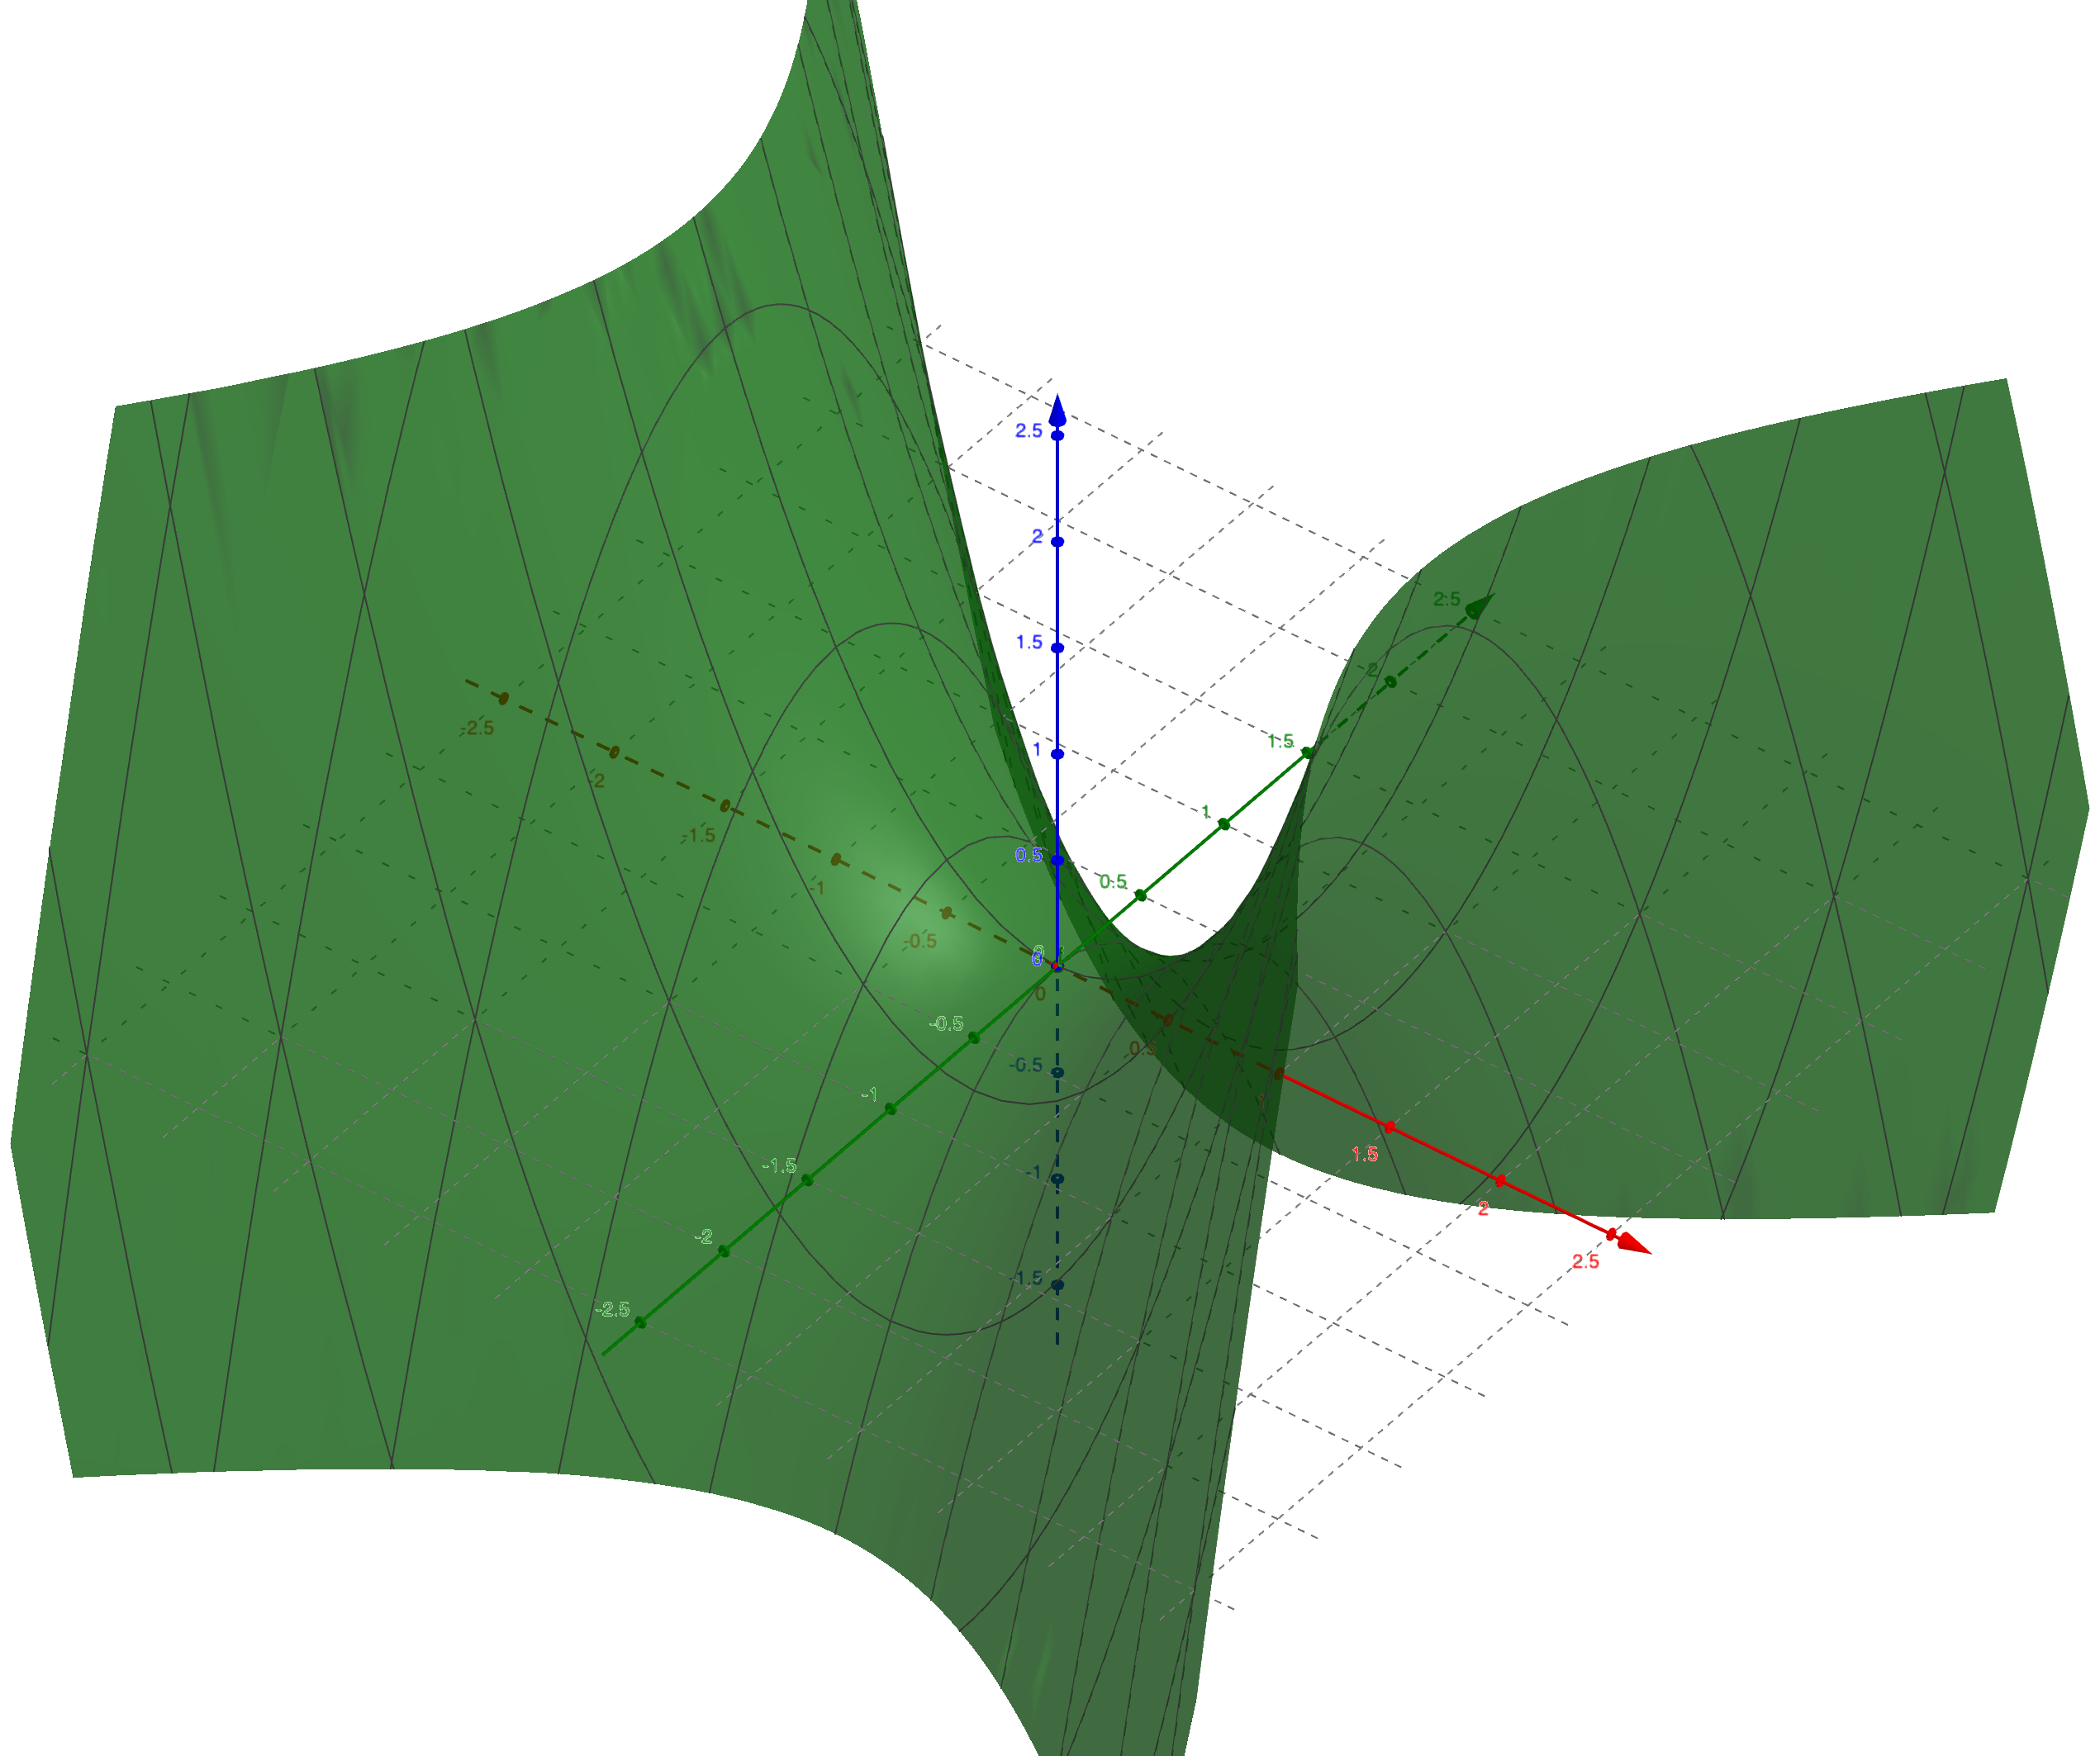
\includegraphics[width = 0.5\textwidth]{media/Sattelpunkt.png}
% \end{center}
\begin{center}
	\begin{tikzpicture}[scale = 0.8]
		\begin{axis}[
				% axis lines=center,
				% axis on top,
				view={120}{30},
				xlabel={$x$},
				ylabel={$y$},
				zlabel={$z$},
				domain=-2:2,
				y domain=-2:2,
				samples=30,
				samples y=30,
				mesh/ordering=y varies,
				colormap/cool,
				surf,
			]
			\addplot3[surf] {x^2 - y^2};
		\end{axis}
	\end{tikzpicture}
\end{center}


Im Folgenden werden wir Funktionen der Form \( f : \mathbb{R}^2 \to \mathbb{R} \) untersuchen – also Funktionen mit zwei reellen Zahlen als Input und einer reellen Zahl als Output. Das ist durchaus sinnvoll: Im Grundlagenfach haben Sie vor allem Funktionen in einer Variable kennengelernt. Bei vielen Anwendungen sind aber mehrere Veränderliche im Spiel.

\begin{itemize}
	\item \textbf{Flächen} (z.\,B.\ in der Computergrafik) können durch Funktionen der Form \( z = f(x, y) \) beschrieben werden.
	\item \textbf{Der Druck eines Gases} ist eine Funktion von Temperatur und Volumen: \( p = p(T, V) \).
	\item \textbf{Der Gewinn eines Unternehmens} hängt von mehreren Faktoren ab: \( G = G(x_1, x_2, \dots, x_k) \).\\
	      Wie kann man die Methoden der Differentialrechnung zur Bestimmung des Extremums für diesen Fall anpassen?
	\item \textbf{Lineare Regression:} Welche Gerade der Form \( y = ax + b \) passt am besten zu den Messresultaten?\\
	      Die Abweichung von Regressionsgerade zu den Messpunkten hängt von den gewählten Koeffizienten \( a \) und \( b \) ab: \( A = A(a, b) \).\\
	      Für welche Wahl von \( a \) und \( b \) ist die Abweichung am kleinsten?
\end{itemize}
\begin{center}
	\begin{tikzpicture}[scale=0.5]
		\begin{axis}[
				axis lines=middle,
				xlabel={$x$},
				ylabel={$y$},
				width=10cm,
				height=6cm,
				%grid=both,
				xmin=0, xmax=6,
				ymin=0, ymax=6,
				%legend style={at={(0.02,0.98)}, anchor=north west}
			]

			% Punktwolke
			\addplot[
				only marks,
				mark=*,
				mark size=2pt,
				color=blue,
			] coordinates {
					(0.5, 1.0)
					(1.0, 1.5)
					(1.5, 2.0)
					(2.0, 2.4)
					(2.5, 3.0)
					(3.0, 3.1)
					(3.5, 3.8)
					(4.0, 4.2)
					(4.5, 4.5)
					(5.0, 5.1)
				};

			% Regressionsgerade: y = 1x + 0.5
			\addplot[
				domain=0:5.5,
				thick,
				red,
			] {x + 0.5};
			%   \addlegendentry{Regressionsgerade}
			%   \addlegendentry{Messpunkte}

		\end{axis}
	\end{tikzpicture}

\end{center}


Wir werden uns zwar auf Funktionen in zwei Variablen beschränken, aber viele der Begriffe und Sätze, die Sie auf den nächsten Seiten kennenlernen werden, lassen sich auch für allgemeinere Funktionen der Form \( f : \mathbb{R}^n \to \mathbb{R} \) verallgemeinern.
%  \clearpage

\section{Graphische Darstellung}

Für Funktionen in einer Variablen kennen wir eine praktische graphische Darstellung: den \textbf{Graphen}.

Der Graph ist die Menge aller Punkte \( (x, y) \) in der Koordinatenebene mit der Eigenschaft, dass \( y = f(x) \) ist.

\begin{center}
	\begin{tikzpicture}[scale = 0.8]
		\begin{axis}[
				axis lines=middle,
				xlabel={$x$},
				ylabel={$y$},
				grid=both,
				domain=-3:3,
				samples=100,
				width=10cm,
				height=5cm,
				axis line style={->},
				enlargelimits=true
			]
			\addplot[blue, thick] {x^2}; % Beispiel: f(x) = x^2

			% Punkt P bei x = 1.5
			\addplot[only marks, mark=*, color=red] coordinates {(1.5, 2.25)};
			\node[color=red, label={below right: \tiny{$P=(1.5,\;f(1.5))$}}] at (axis cs:1.5,2.25) {};
		\end{axis}
	\end{tikzpicture}

\end{center}


Analog lassen sich Funktionen der Form \( f(x, y) \) darstellen. Der Graph ist dann wiederum die Menge aller Punkte \( (x, y, z) \) im dreidimensionalen Raum mit der Eigenschaft, dass \( z = f(x, y) \) ist.
\begin{center}

	\begin{tikzpicture}[scale = 0.8]
		\begin{axis}[
				view={120}{30},
				xlabel={$x$},
				ylabel={$y$},
				zlabel={$z$},
				domain=-2:2,
				y domain=-2:2,
				samples=30,
				samples y=30,
				axis lines=center,
				axis on top,
				axis line style={->},
				colormap/cool,
				width=10cm,
				height=8cm,
			]
			\addplot3[surf] {x^2 - y^2};
			% Punkt P bei (-1, 1): f(-1,1) = 0
			\addplot3[only marks, mark=*, color=red, mark size=2pt]
			coordinates {(-1, 1, 0)};
			\node[below] at (axis cs:-1,1,0) {\tiny{$P=(-1,\;1,\;f(-1,1))$}};
		\end{axis}
	\end{tikzpicture}
\end{center}
Weil die Koordinatenachsen manchmal die Darstellung stören, werden Sie teilweise in eine Box rund um den Graphen gezeichnet:
\begin{tikzpicture}[scale = 0.8]
	\begin{axis}[
			view={120}{30},
			xlabel={$x$},
			ylabel={$y$},
			zlabel={$z$},
			domain=-2:2,
			y domain=-2:2,
			samples=30,
			samples y=30,
			% axis lines=center,
			% axis on top,
			axis line style={->},
			colormap/cool,
			width=10cm,
			height=8cm,
		]
		\addplot3[surf] {x^2 - y^2};
		% Punkt P bei (-1, 1): f(-1,1) = 0
		\addplot3[only marks, mark=*, color=red, mark size=2pt]
		coordinates {(-1, 1, 0)};
		\node[below] at (axis cs:-1,1,0) {\tiny{$P=(-1,\;1,\;f(-1,1))$}};
	\end{axis}
\end{tikzpicture}

% \begin{bsp}
% {Der Graph der Funktion $f(x,y)=x^2+ \frac{1}{2} y^2$}{}
% \begin{center}

%     \begin{tikzpicture}
%         \begin{axis}[
%           view={120}{30},
%           xlabel={$x$},
%           ylabel={$y$},
%           zlabel={$z$},
%           domain=-2:2,
%           y domain=-2:2,
%           samples=30,
%           samples y=30,
%         %   axis lines=center,
%         %   axis on top,
%           axis line style={->},
%           colormap/cool,
%           width=10cm,
%           height=8cm,
%         ]
%           \addplot3[surf] {x^2 +0.5* y^2};
%         \end{axis}
%       \end{tikzpicture}
%     \end{center}
% \end{bsp}
% \begin{bsp}
%     {Der Graph der Funktion $f(x,y)=-xy$}{}
%     \begin{center}

%         \begin{tikzpicture}
%             \begin{axis}[
%               view={120}{15},
%               xlabel={$x$},
%               ylabel={$y$},
%               zlabel={$z$},
%               domain=-2:2,
%               y domain=-2:2,
%               samples=30,
%               samples y=30,
%             %   axis lines=center,
%             %   axis on top,
%               axis line style={->},
%               colormap/cool,
%               width=10cm,
%               height=8cm,
%             ]
%               \addplot3[surf] {-x*y};
%             \end{axis}
%           \end{tikzpicture}
%         \end{center}
% \end{bsp}
% \begin{bsp}
%     {Der Graph der Funktion $f(x,y)=\sqrt{4-x^2-y^2}$}{}
%     \begin{center}

%         \begin{tikzpicture}
%             \begin{axis}[
%               view={130}{15},
%               xlabel={$x$},
%               ylabel={$y$},
%               zlabel={$z$},
%               %axis lines=center,
%               axis line style={->},
%               ticks=none,
%               samples=40,
%               samples y=30,
%               width=10cm,
%               height=8cm,
%               colormap/cool,
%             ]
%               % Parametrische Darstellung der oberen Halbkugel (r = 2)
%               \addplot3[
%                 surf,
%                 domain=0:90,
%                 y domain=130:490,
%                 variable=\t,
%                 variable y=\p,
%               ]
%               (
%                 {2*sin(\t)*cos(\p)},
%                 {2*sin(\t)*sin(\p)},
%                 {2*cos(\t)}
%               );
%             \end{axis}
%           \end{tikzpicture}
%         \end{center}
% \end{bsp}


Eine Möglichkeit zur Veranschaulichung solcher Graphen besteht darin, \textbf{vertikale Schnitte} des Graphen zu betrachten.
Genauer: Wir schneiden den Graphen mit Ebenen, die parallel zur \( xz \)-Ebene oder zur \( yz \)-Ebene verlaufen. Im ersten Fall gilt: \( y = y_0 = \text{konstant} \). Im zweiten Fall gilt: \( x = x_0 = \text{konstant} \)

\begin{definition}
	{Schnittkurven}{}
	Sei \( f : \mathbb{R}^2 \to \mathbb{R},\ (x, y) \mapsto f(x, y) \), eine Funktion in zwei Variablen.

	Für fixiertes \( y_0 \) (bzw. \( x_0 \)) ist die \textbf{Schnittkurve} definiert als der Graph der Funktion
	\[
		x \mapsto f(x, y_0) \quad \text{bzw.} \quad y \mapsto f(x_0, y).
	\]

	Für jedes fixierte \( y_0 \) oder \( x_0 \) gibt es also eine eigene Schnittkurve. Stellen wir mehrere dieser Kurven zusammen, so erhalten wir ein \textbf{Schnittkurvendiagramm}.

\end{definition}
\begin{bsp}
	{Schnittkurvendiagramm der Funktion $V(x,y) = \frac{1}{2}x^2+y^2$}{}
	Wenn wir $x_0$ fixieren erhalten wir lauter quadratische Funktionen $y \mapsto V(x_0, y)$. Deren Graphen sind Parabeln. In der Abbildung sind die Schnittkurven für $x_0=0, \pm1, \pm2$ dargestellt.
	\begin{center}
		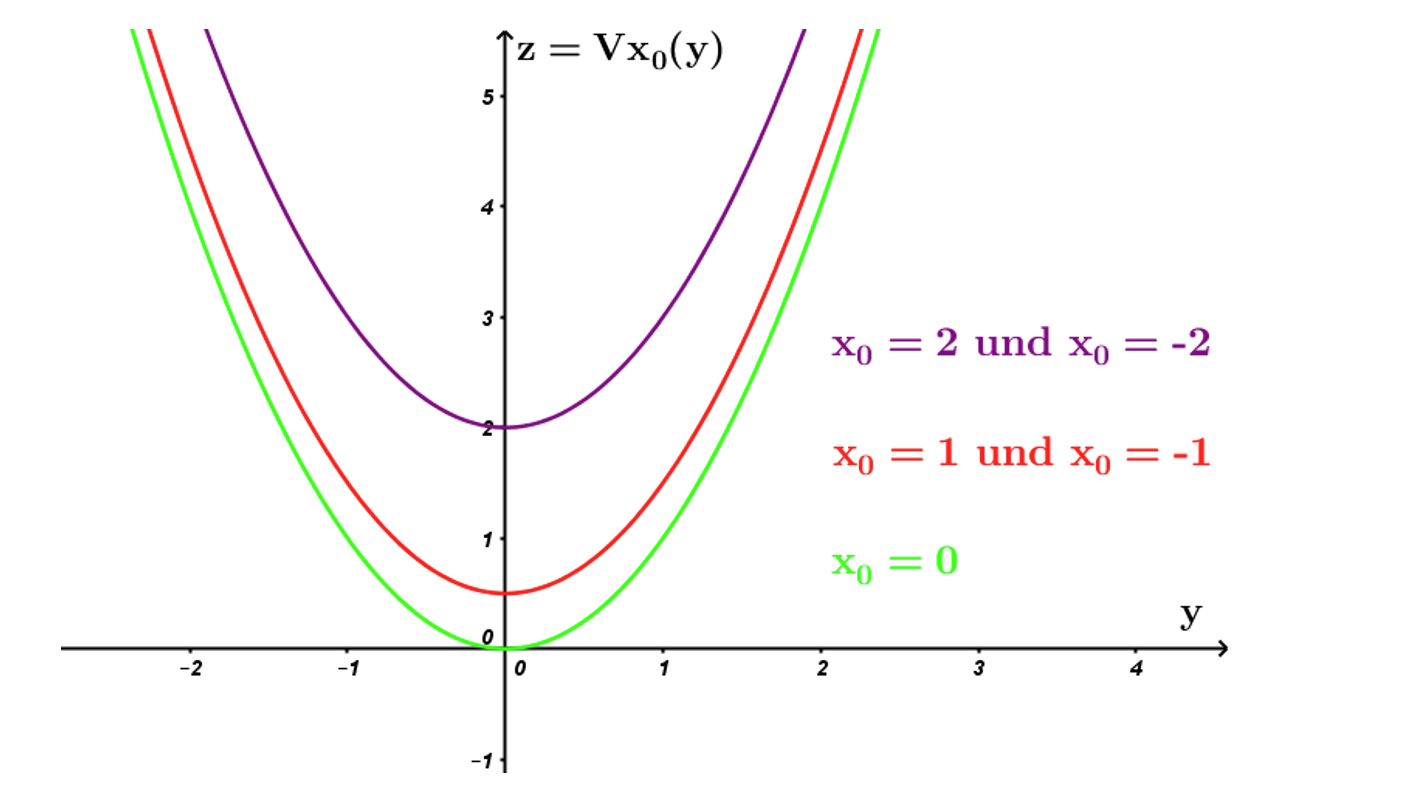
\includegraphics[width = 0.5\textwidth]{media/SchnittkurvenBsp.png}
	\end{center}
	Die gleichen Kurven im Raum platziert:
	\begin{center}
		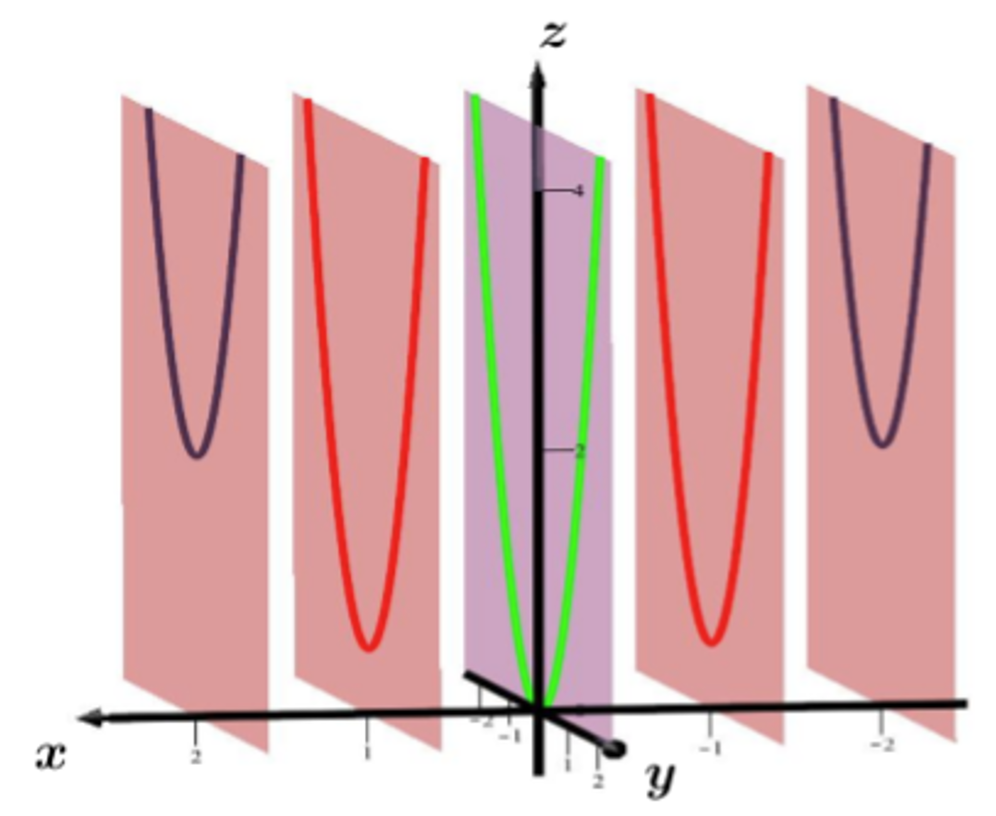
\includegraphics[width = 0.5\textwidth]{media/Schnittkurven-im-Raum.png}
	\end{center}

\end{bsp}
\clearpage
Eine andere Möglichkeit, sich ein Bild von solchen Graphen zu machen sind die \textbf{Niveaulinien}. Dieses Prinzip kennen wir als Höhenlinien auf einer Landkarte.

\begin{definition}
	{Niveaulinien}{}
	Sei \( f : \mathbb{R}^2 \to \mathbb{R},\ (x, y) \mapsto f(x, y) \), eine Funktion in zwei Variablen.

	\textbf{Niveaulinien} von \( f \) bestehen aus allen Inputs, welche auf den gleichen Output führen – das heisst, aus den Lösungen \( (x, y) \) der Gleichung
	\[
		f(x, y) = z_0,
	\]
	wobei \( z_0 \) fixiert, also konstant, ist.

	Niveaulinien sind also Teilmengen der \( xy \)-Ebene, welche auf die gleiche „Höhe“ abgebildet werden.

\end{definition}
% In einigen unserer Beispiele werden die Lösungen solcher Gleichungen \textbf{Kegelschnitte} sein. Hier sind die wichtigsten Formen zusammengestellt:

% \begin{description}
%   \item[Parabeln:] 
%   \[
%   y = ax^2 \quad \text{oder} \quad x = ay^2
%   \]

%   \item[Ellipsen:] 
%   \[
%   \frac{x^2}{a^2} + \frac{y^2}{b^2} = 1
%   \]

%   \item[Hyperbeln:] 
%   \[
%   \frac{x^2}{a^2} - \frac{y^2}{b^2} = 1 \quad \text{oder} \quad -\frac{x^2}{a^2} + \frac{y^2}{b^2} = 1
%   \]
% \end{description}

\begin{bsp}
	{Niveaulinien der Funktion $V(x,y) = \frac{1}{2}x^2+y^2$ }{}
	Für den konstanten Output \( z_0 := c \) ergibt sich:

	\[
		V(x, y) = \frac{x^2}{2} + y^2 = c \iff \frac{x^2}{( \sqrt{2c} )^2} + \frac{y^2}{( \sqrt{c} )^2} = 1
	\]

	Dies sind \textbf{Ellipsen} mit Halbachsenlängen
	\[
		a = \sqrt{2c} \quad \text{und} \quad b = \sqrt{c}.
	\]
	\begin{center}
		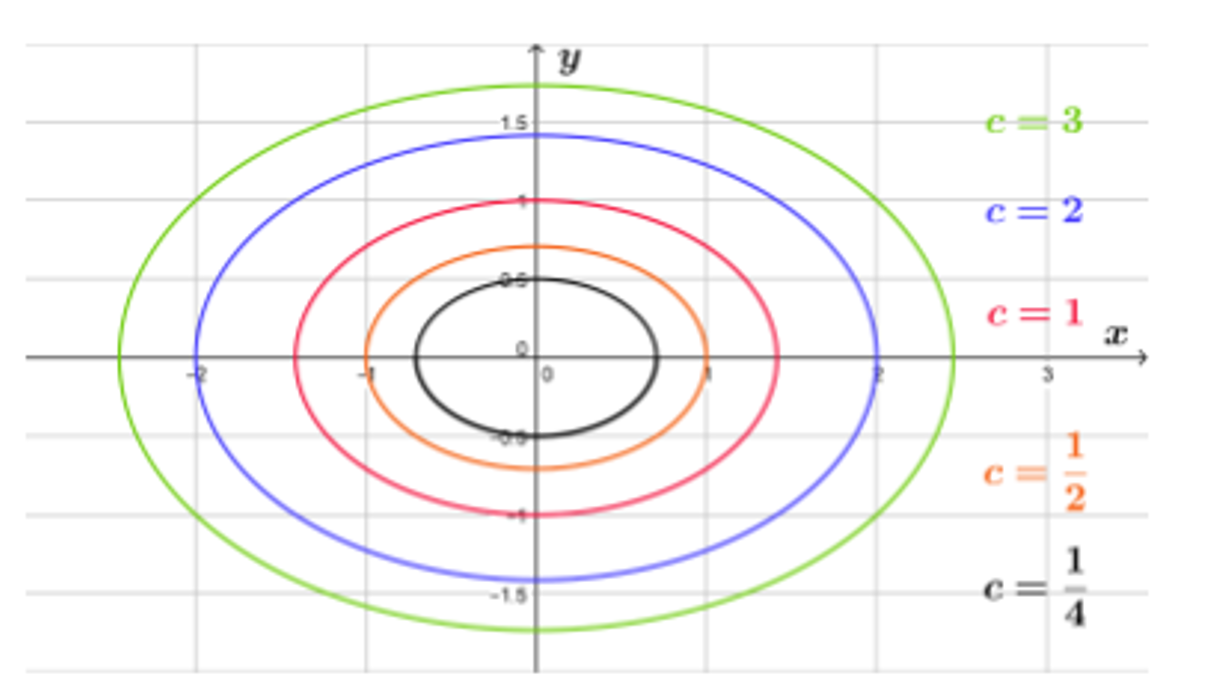
\includegraphics[width = 0.4\textwidth]{media/NiveaulinienBsp.png}
	\end{center}
\end{bsp}

Aus Schnittkurven und Niveaulinien ”verstehen” wir den Graphen von $V$:
\begin{center}
	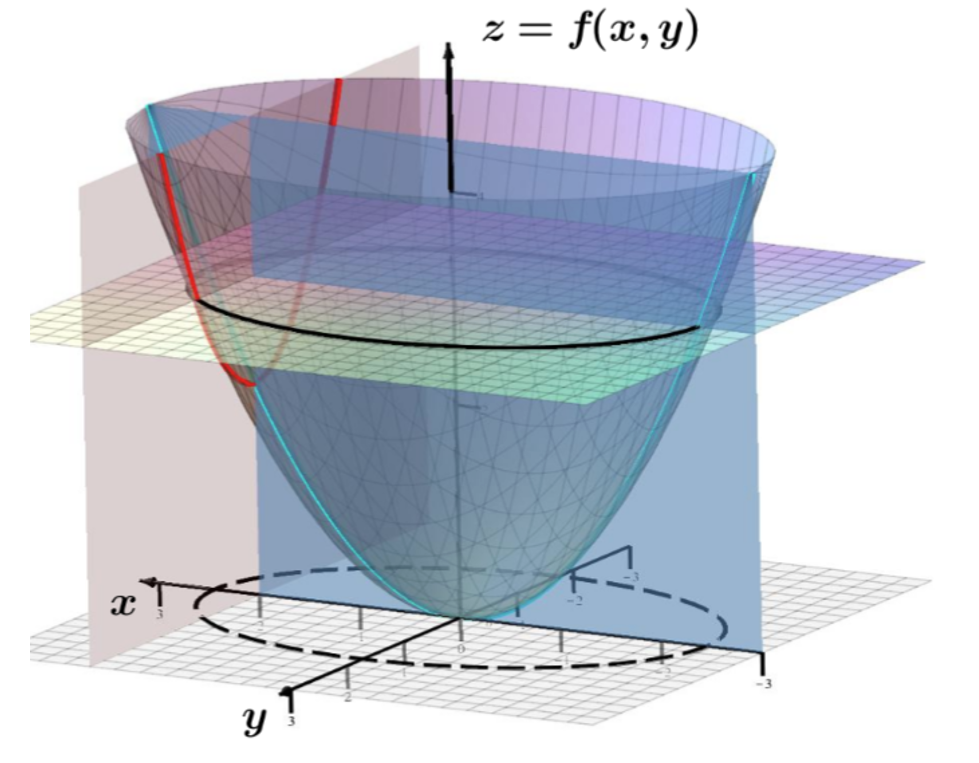
\includegraphics[width = 0.4 \textwidth]{media/GraphAusSchnittkurveNiveaulinien.png}
\end{center}





\begin{ueb}
	{}{}
	\begin{enumerate}
		\item Gegeben ist die Funktion \( f(x, y) = x^2 + 4xy + y^2 - \ln(1 + x^2) \). Prüfen Sie, ob der Punkt \( P = (0, -3) \) auf der Niveaulinie zum Niveau \( z = 9 \) liegt.

		\item Erstellen Sie die Schnittkurvendiagramme der folgenden Funktionen %, bestimmen Sie ihre Niveaulinien 
		      und skizzieren Sie ihre Graphen. Wählen Sie als Schnittkurven die Graphen der Funktionen $x \mapsto f(x, y_0)$ mit $y_0 = -1, 0, 1$
		      \begin{enumerate}
			      %\item \( f(x, y) = \sqrt{x^2 + y^2} \)
			      \item \( f(x, y) = x^2 + 1 \)
			      \item \( f(x, y) = x^2 + y \)
		      \end{enumerate}
		\item Zeichnen Sie das \textbf{Niveaulinienportrait} der folgenden Funktionen. Können Sie sich den Graphen der Funktion damit vorstellen? Überprüfen Sie die Vorstellung, indem Sie den Graphen mit \href{https://www.geogebra.org/calculator}{Geogebra} zeichnen.

		      \begin{enumerate}
			      \item \( f(x, y) = \sqrt{x^2 + y^2} \)
			      \item \( f(x, y) = 2x + 3y \)
			      \item \( g(x, y) = xy \)
		      \end{enumerate}
	\end{enumerate}
\end{ueb}
\clearpage
\emph{Lösungen}
\begin{enumerate}
	\item \begin{align*}
		      f(0, -3)
		       & = (0)^2 + 4 \cdot 0 \cdot (-3) + (-3)^2 - \ln(1 + 0^2) \\
		       & = 0 + 0 + 9 - \ln(1)                                   \\
		       & = 9 - 0                                                \\
		       & = 9
	      \end{align*}

	      Da \( f(0, -3) = 9 \), liegt der Punkt \( P = (0, -3) \) tatsächlich auf der Niveaulinie zum Niveau \( z = 9 \).
	\item Schnittkurvendiagramme:
	      \begin{enumerate}
		      \item \( f(x, y) = x^2 + 1 \)

		            \begin{figure}[h!]
			            \centering
			            \begin{subfigure}[t]{0.48\textwidth}
				            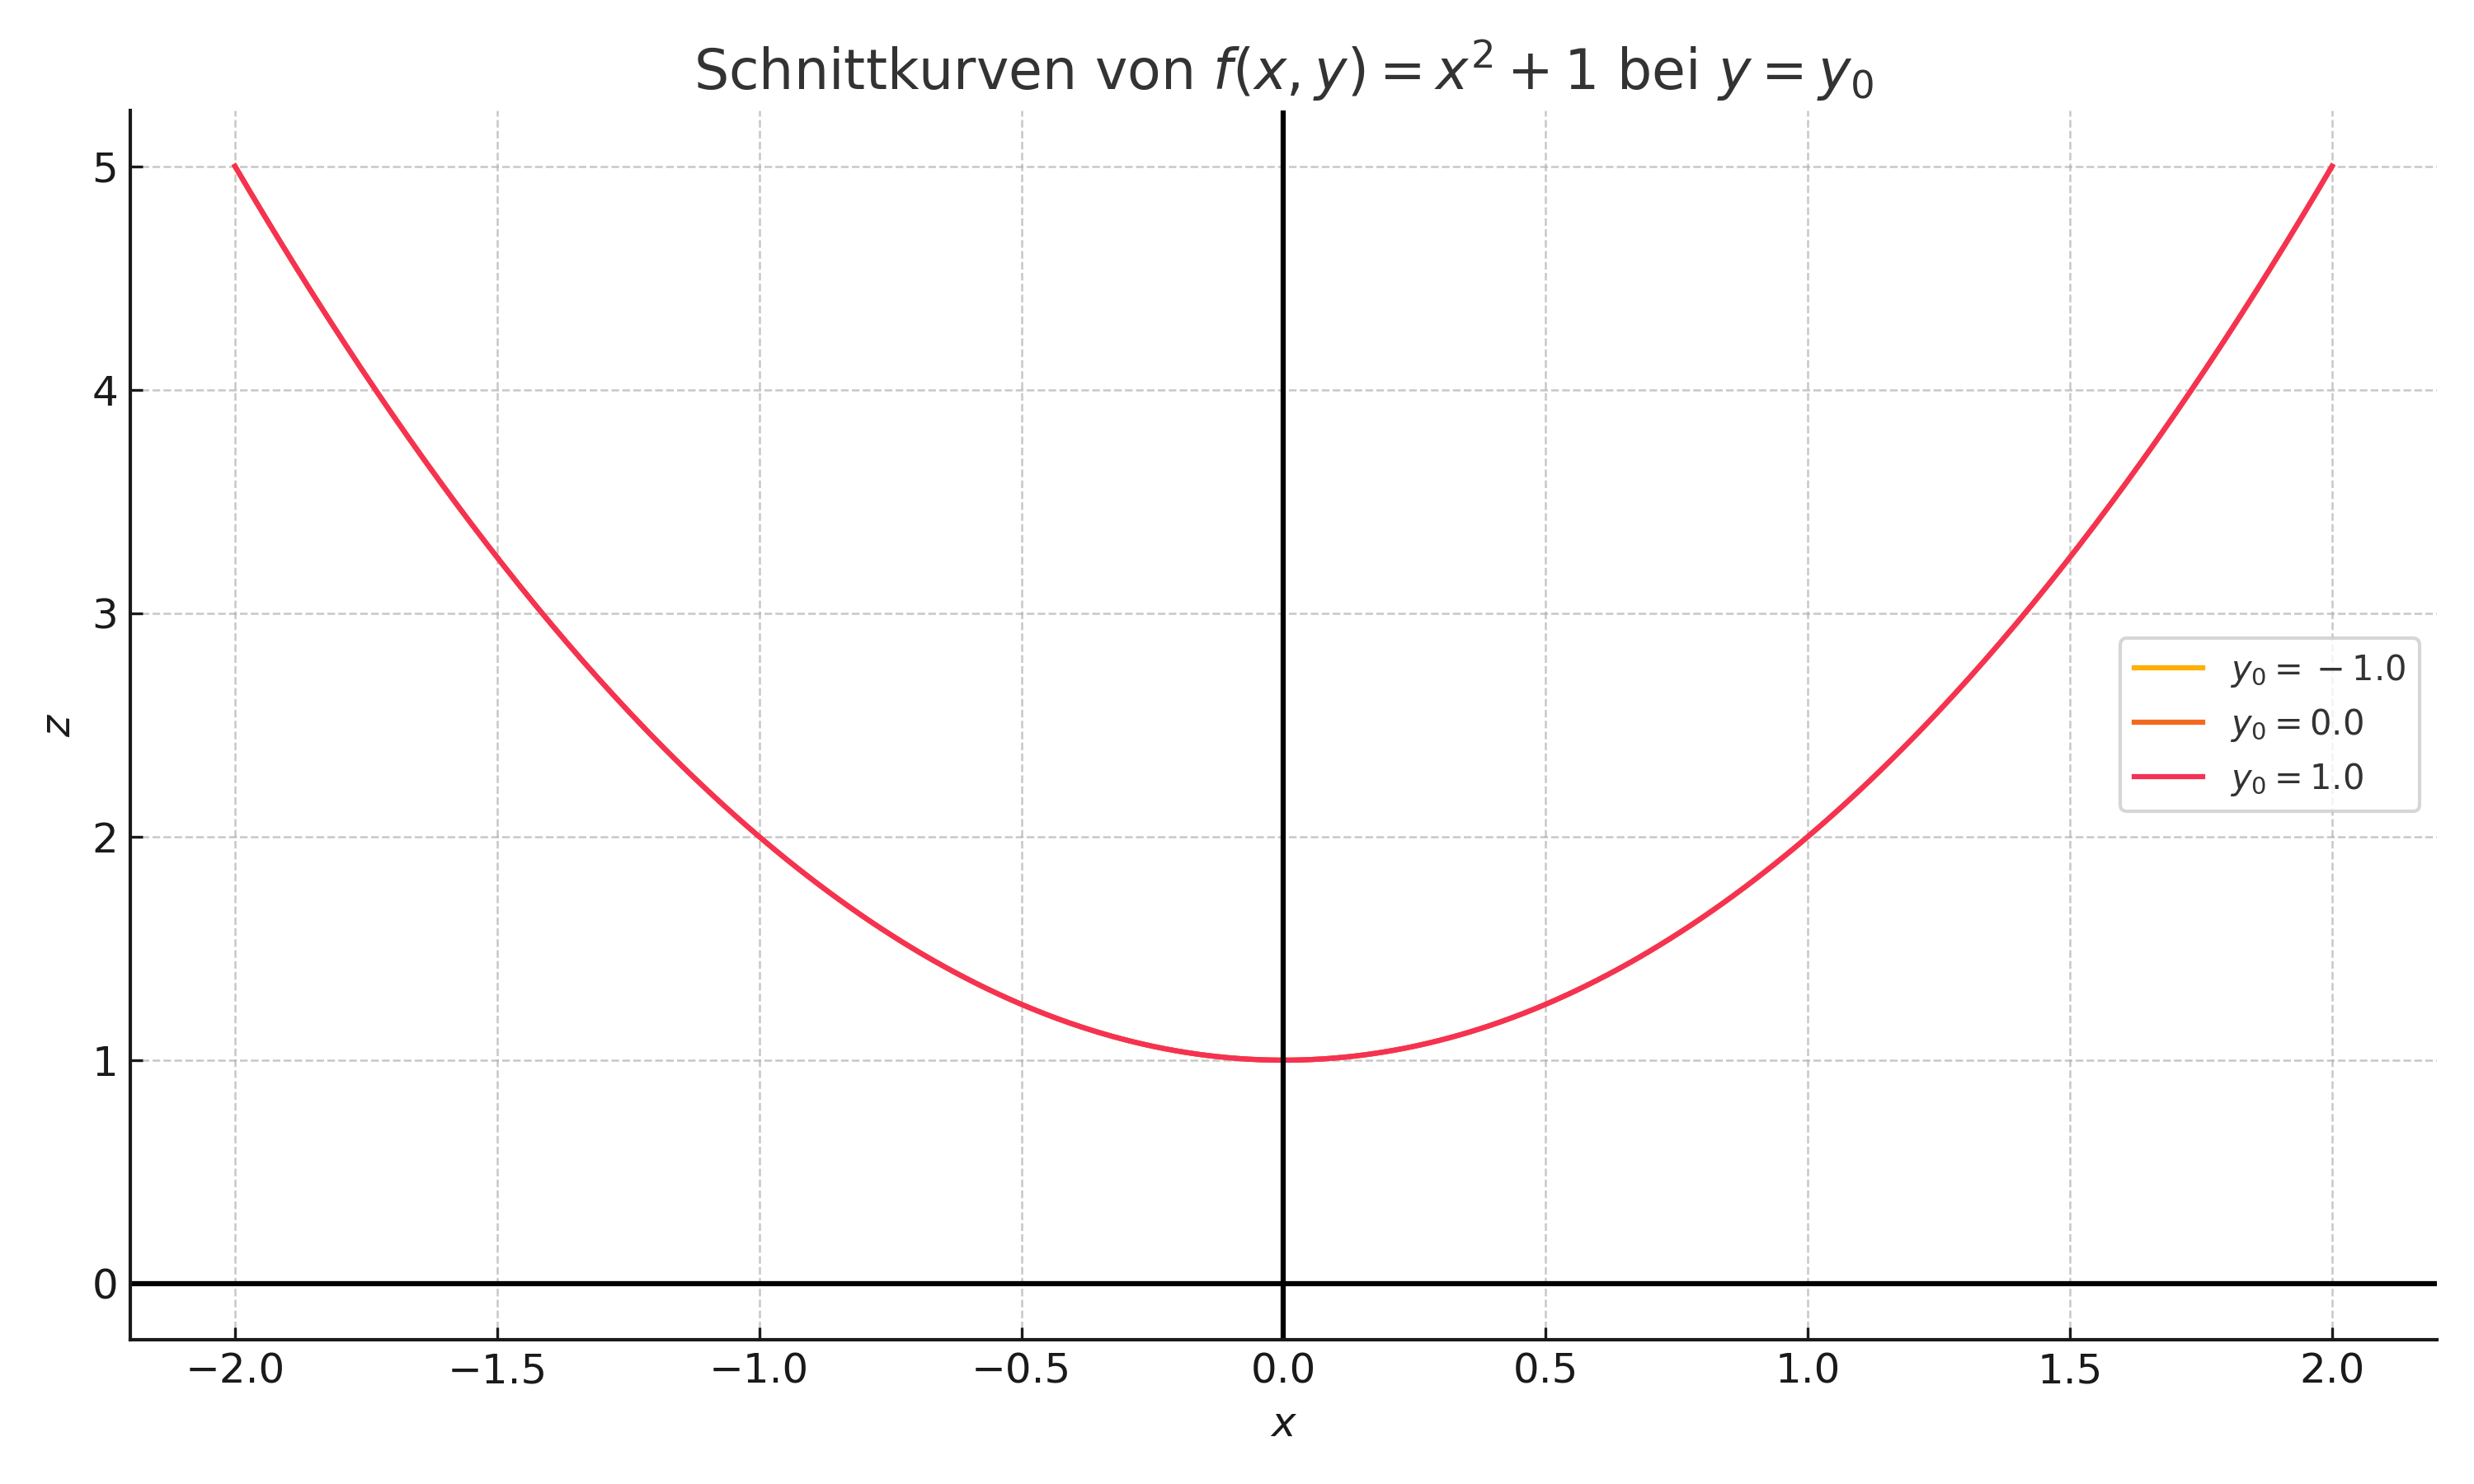
\includegraphics[width=\linewidth]{media/ueb1/schnitt_f1_labeled.png}
				            \caption*{Schnittkurven bei festen \( y_0 \)}
			            \end{subfigure}
			            \hfill
			            \begin{subfigure}[t]{0.48\textwidth}
				            \centering
				            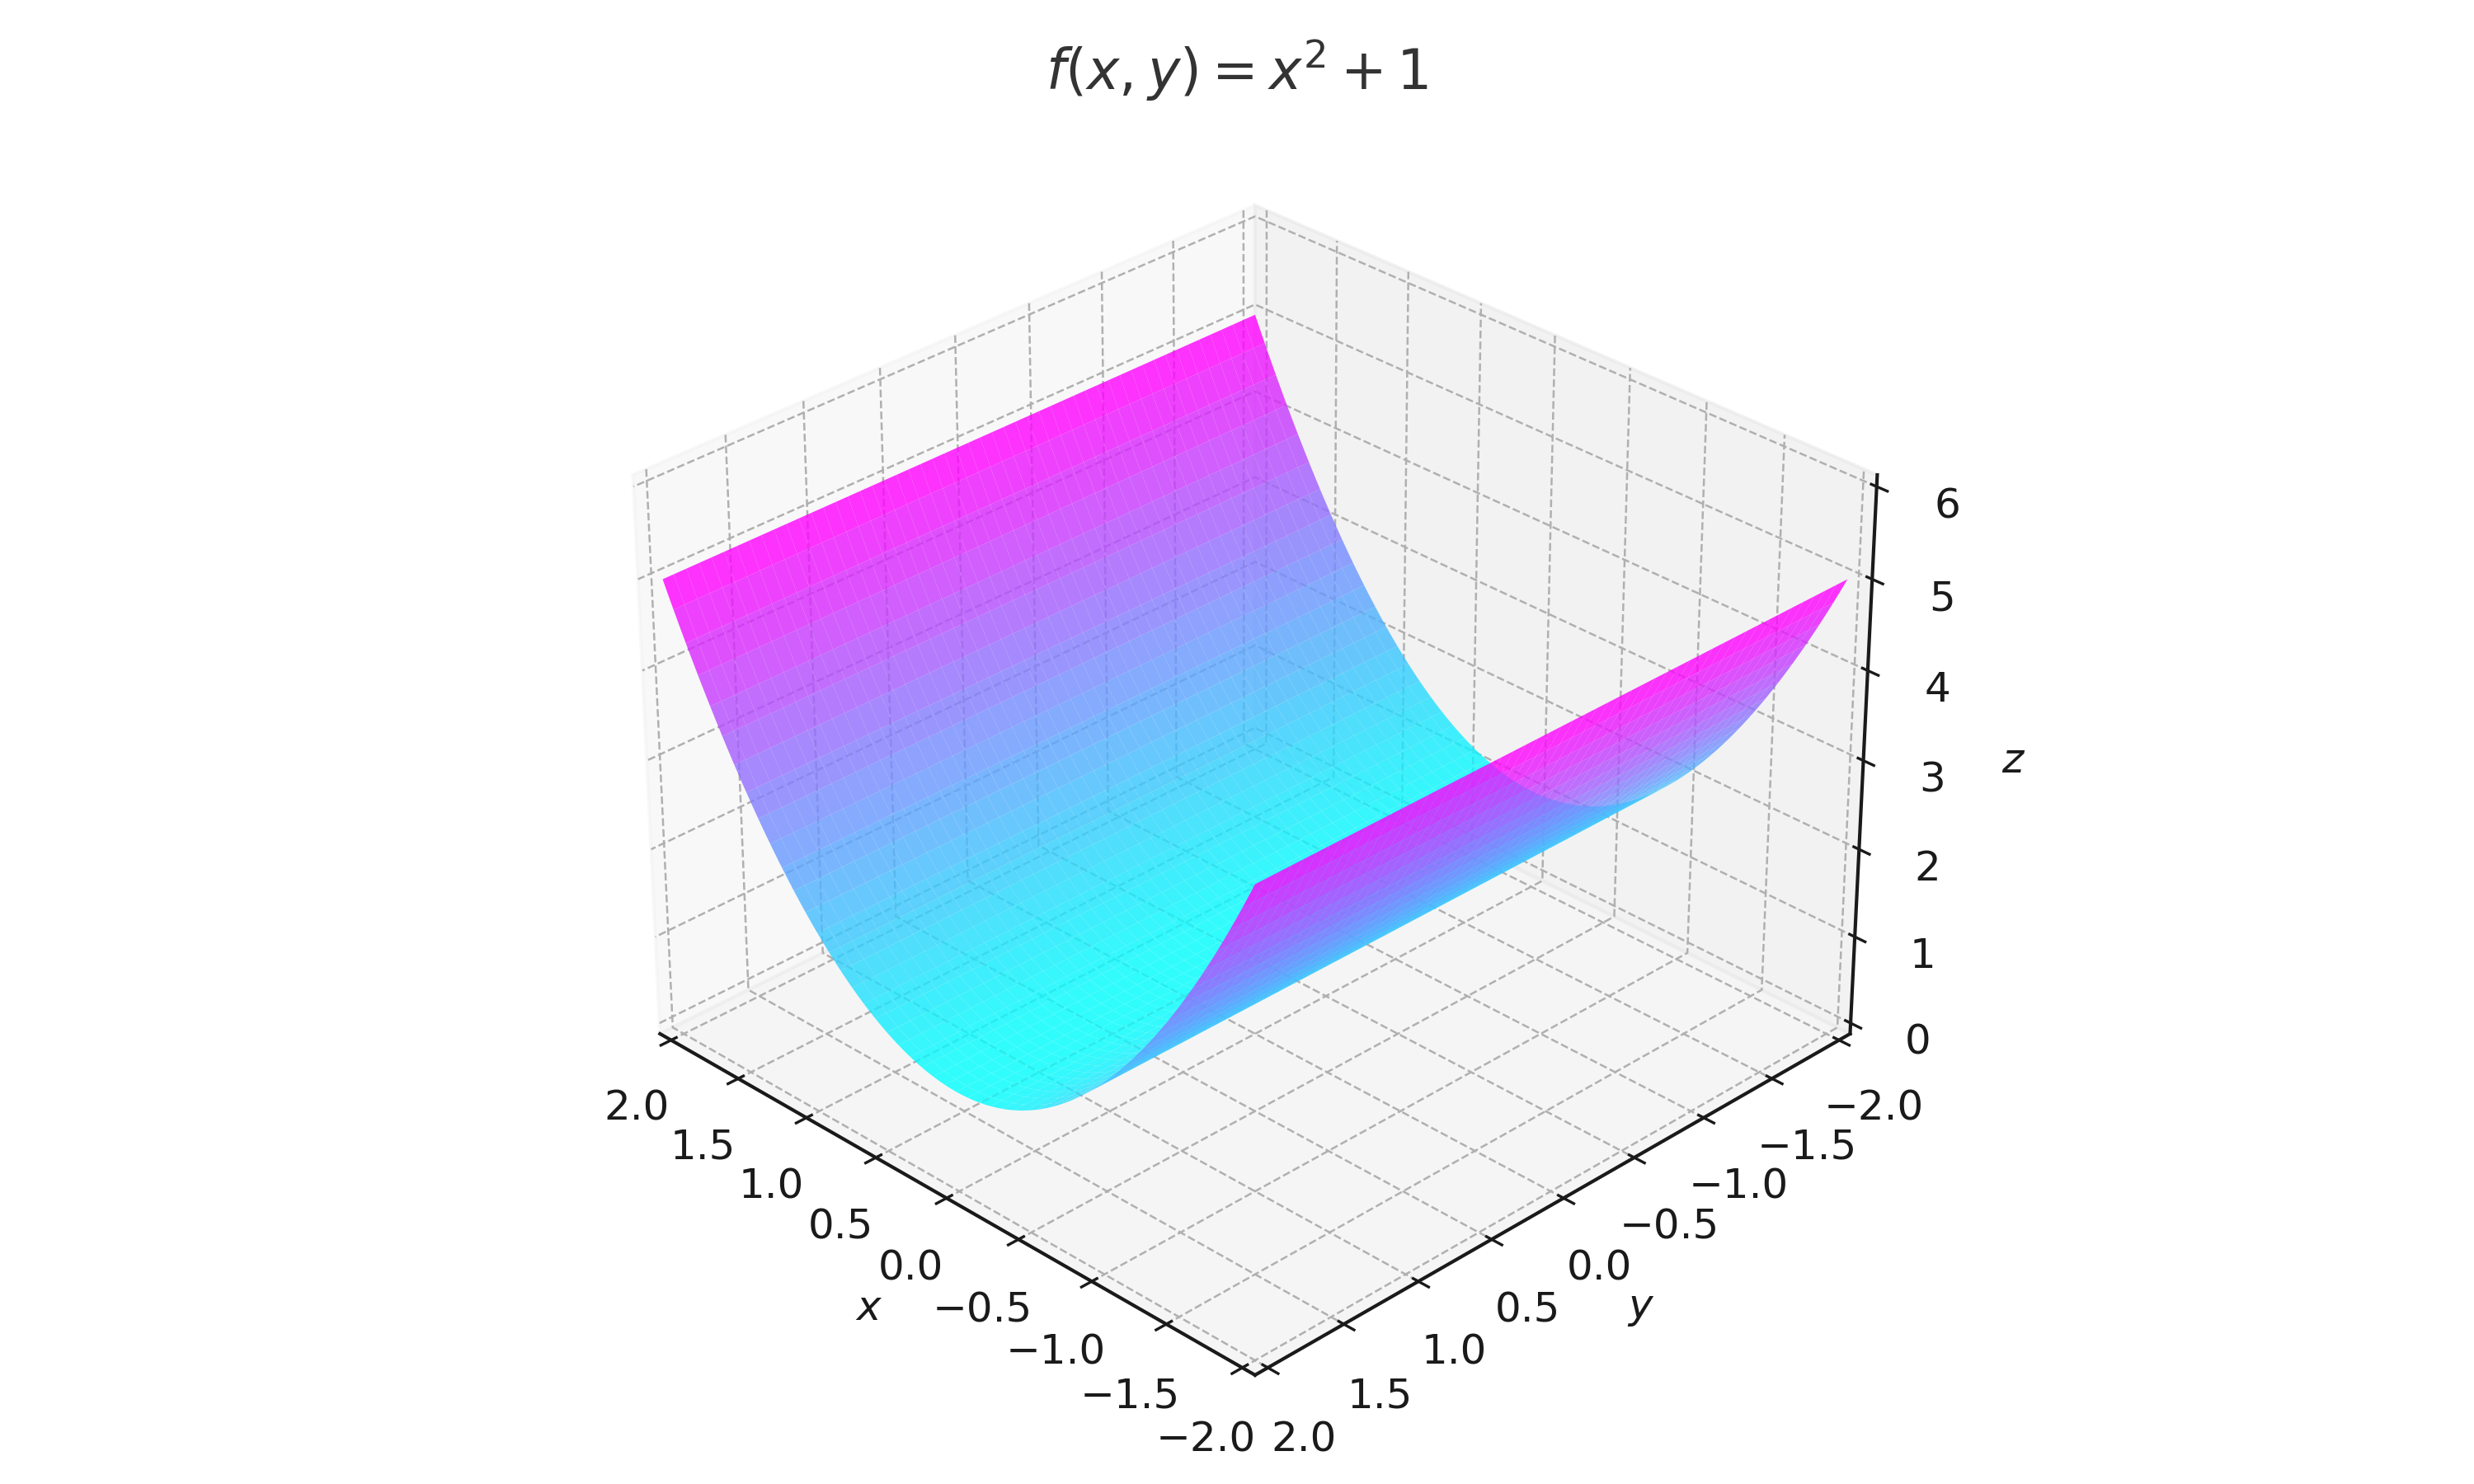
\includegraphics[width=\linewidth]{media/ueb1/graph_f1_labeled.png}
				            \caption*{Graph der Funktion \( f(x, y) \)}
			            \end{subfigure}
			            \caption{Visualisierung von \( f(x, y) = x^2 + 1 \)}
			            % \begin{subfigure}[t]{0.48\textwidth}
			            %   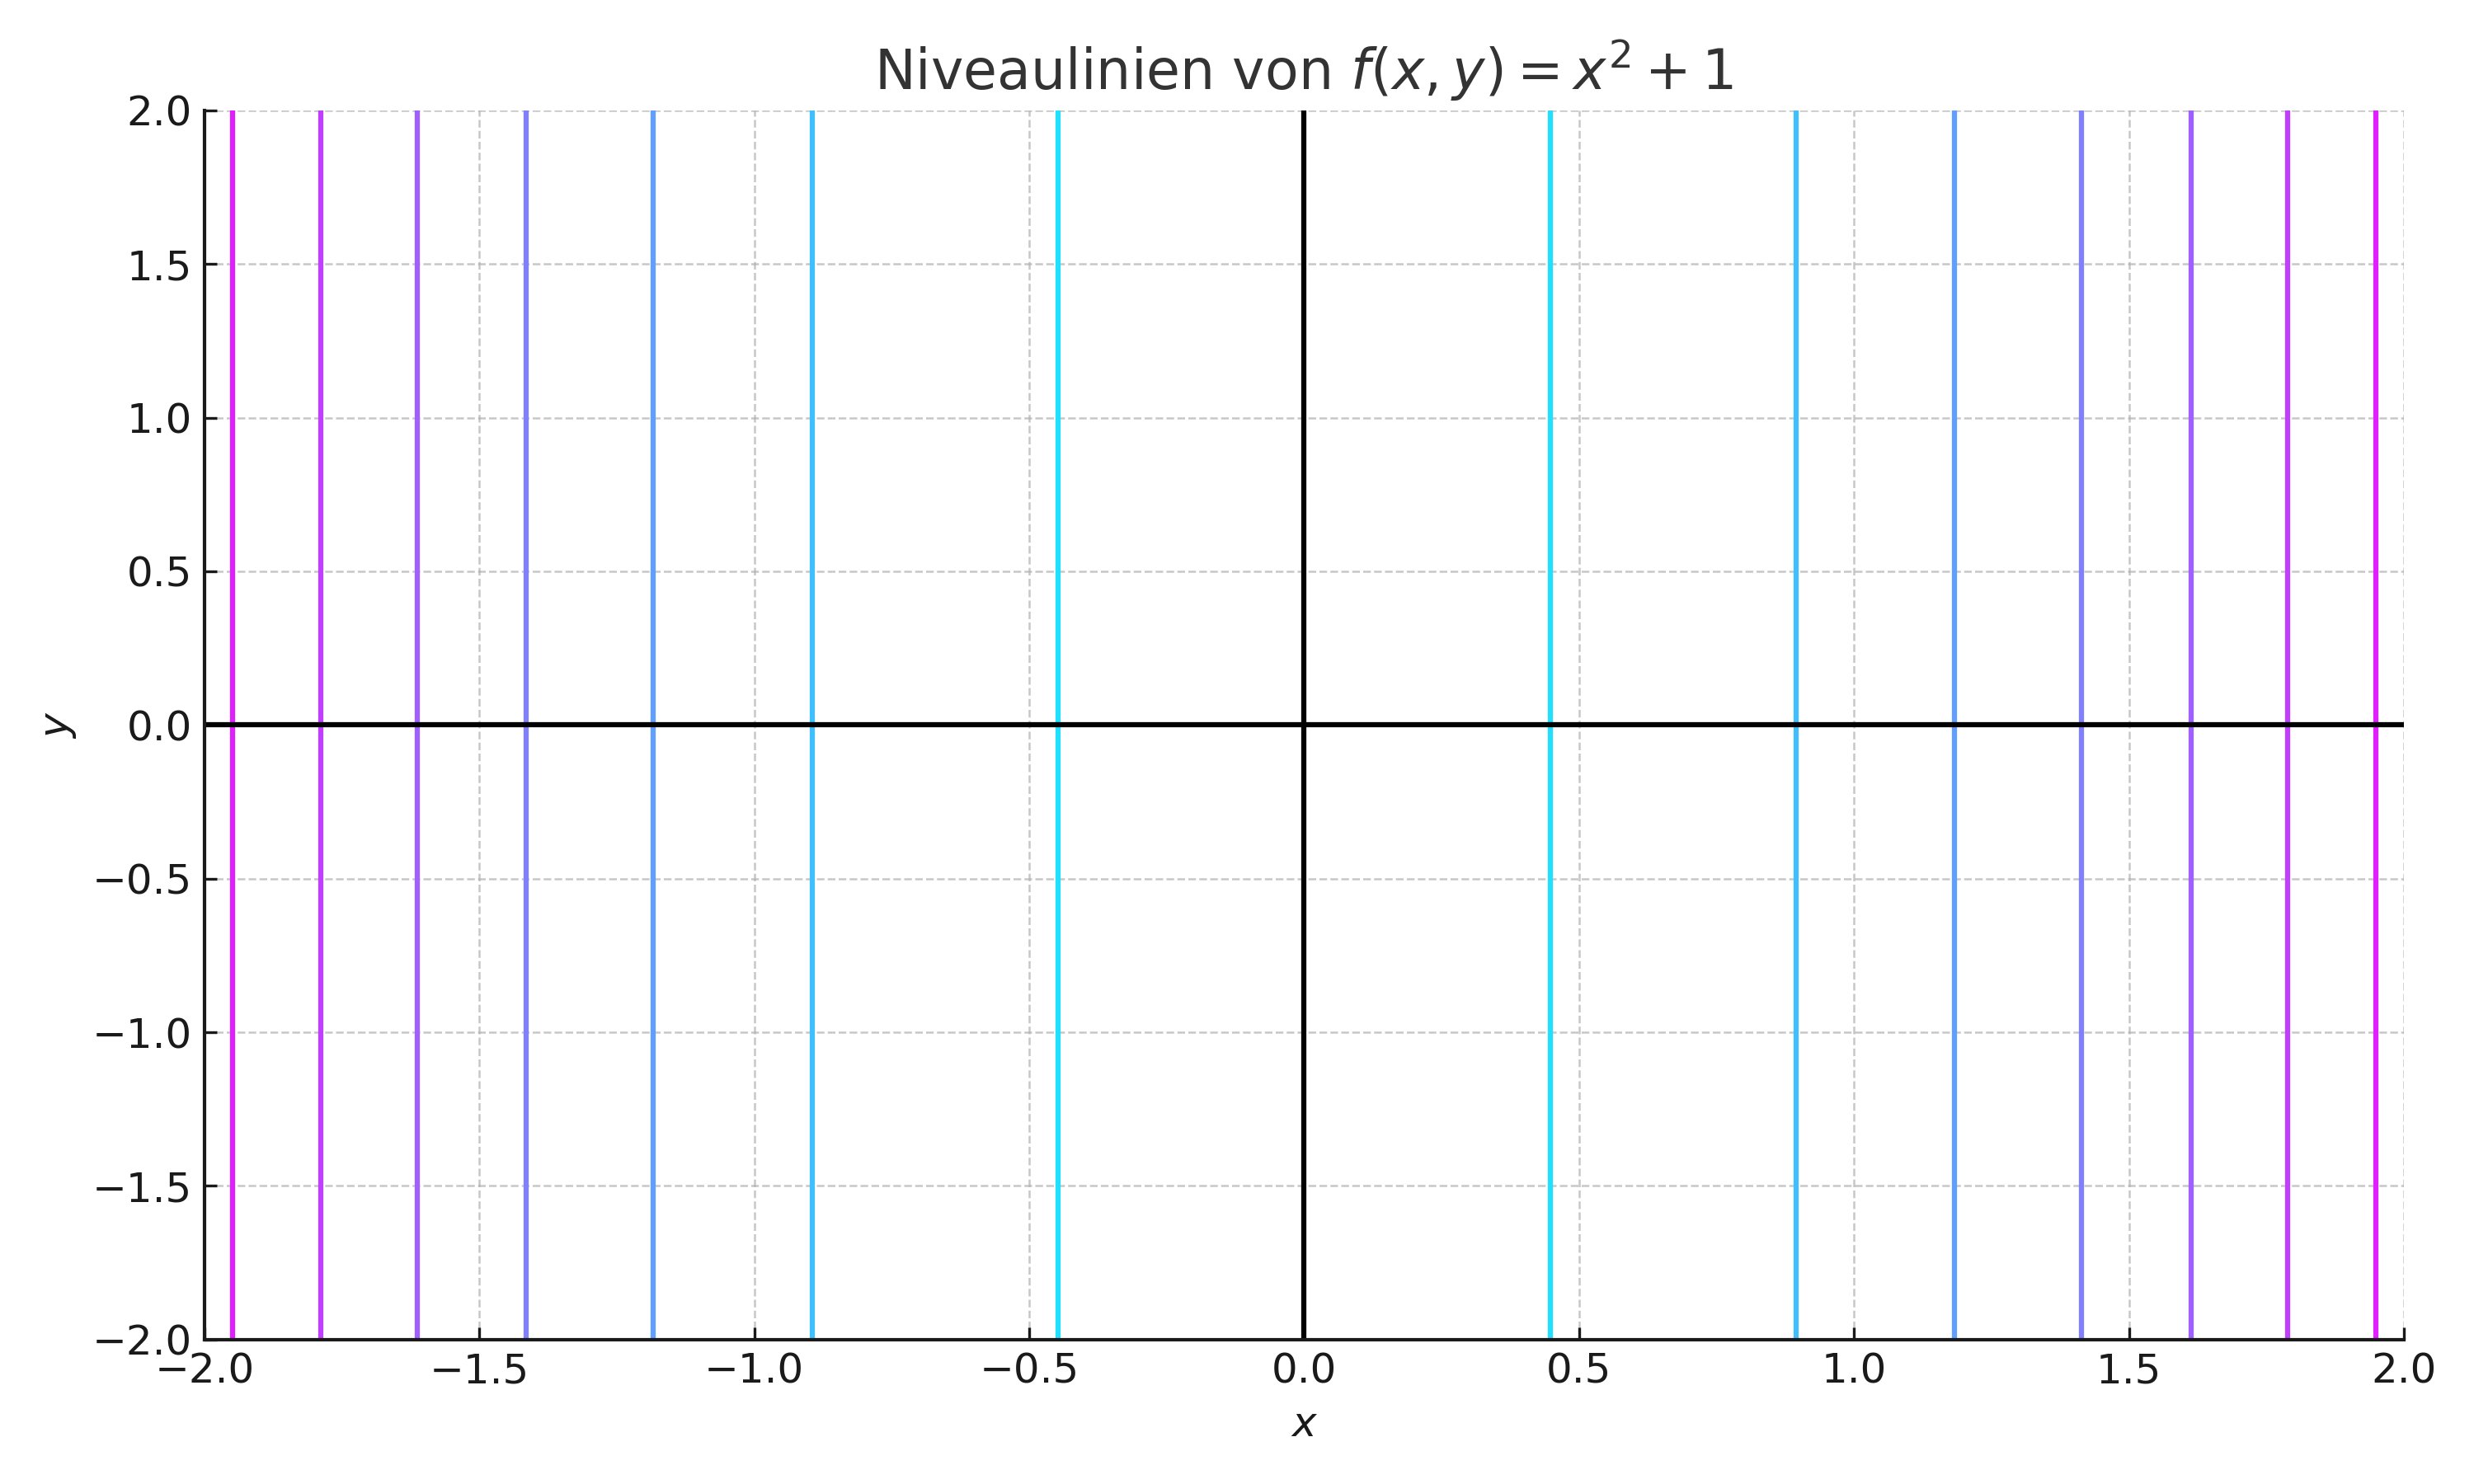
\includegraphics[width=\linewidth]{media/ueb1/niveau_f1_labeled.png}
			            %   \caption{Niveaulinien in der \( xy \)-Ebene}
			            % \end{subfigure}

			            % \vspace{1em}

		            \end{figure}
		      \item \( f(x, y) = x^2 + y \)

		            \begin{figure}[h!]
			            \centering
			            \begin{subfigure}[t]{0.48\textwidth}
				            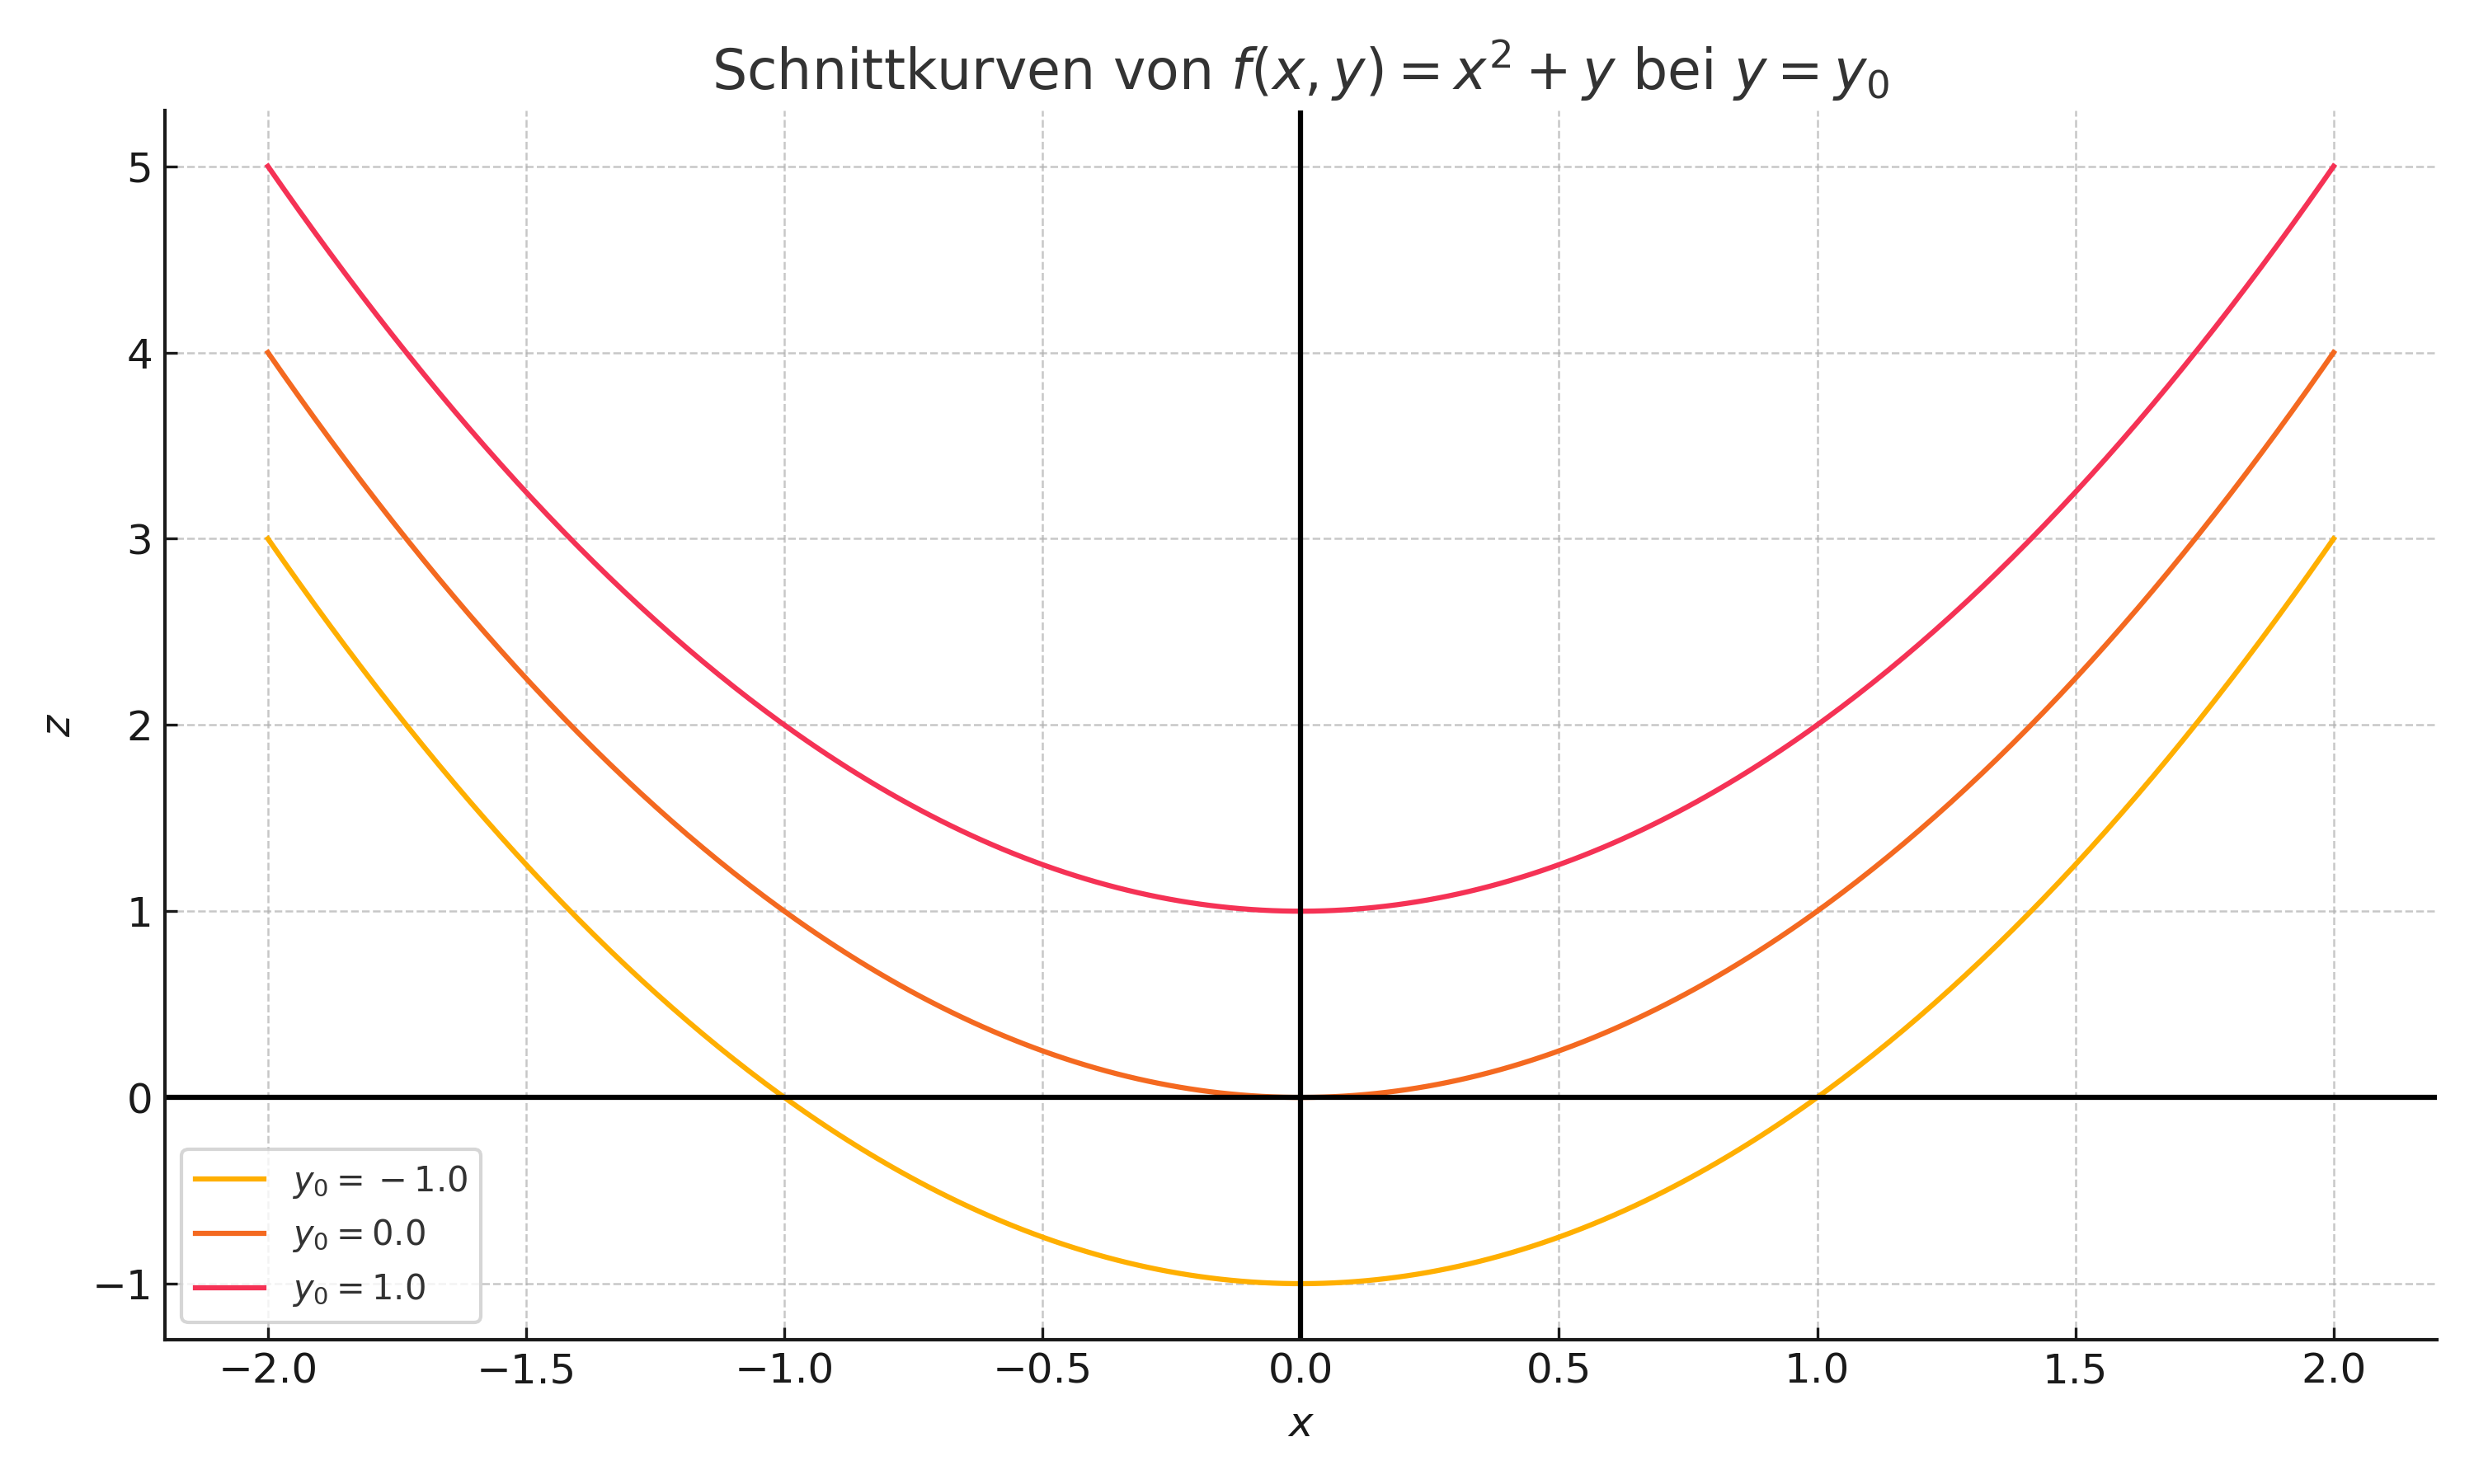
\includegraphics[width=\linewidth]{media/ueb1/schnitt_f2_labeled.png}
				            \caption*{Schnittkurven bei festen \( y_0 \)}
			            \end{subfigure}
			            \hfill
			            \begin{subfigure}[t]{0.48\textwidth}
				            \centering
				            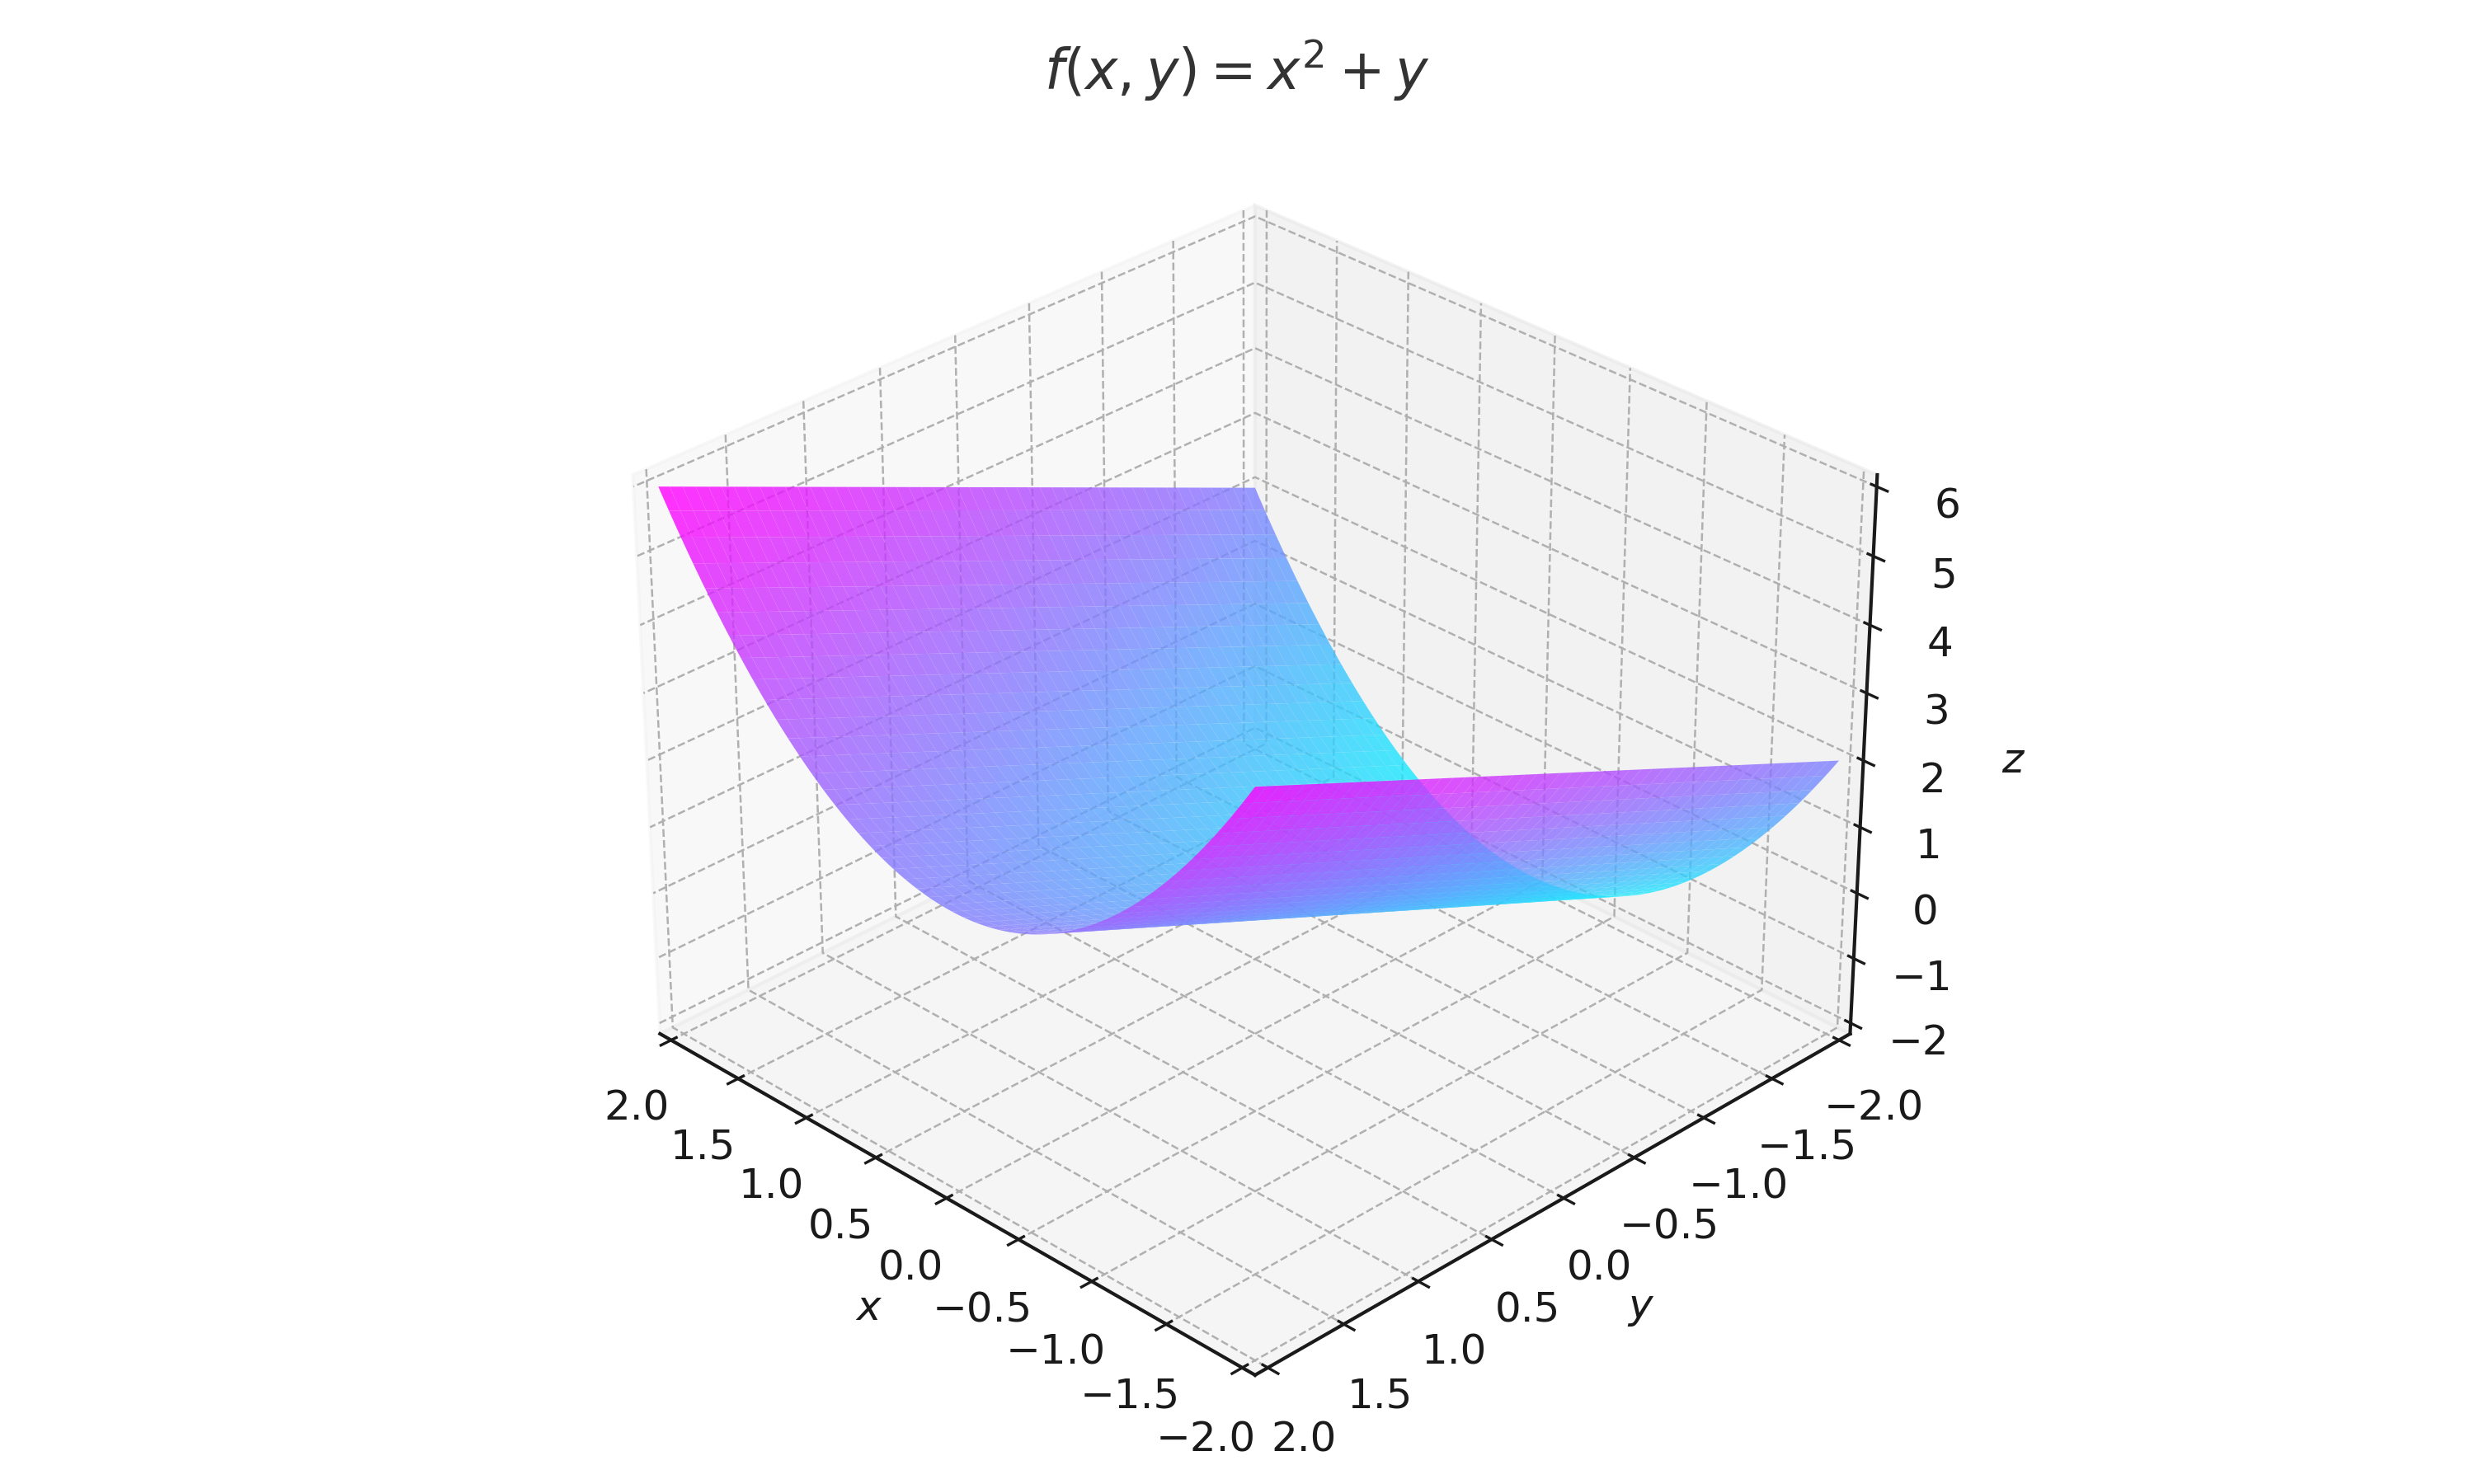
\includegraphics[width=\linewidth]{media/ueb1/graph_f2_labeled.png}
				            \caption*{Graph der Funktion \( f(x, y) \)}
			            \end{subfigure}

			            \caption{Visualisierung von \( f(x, y) = x^2 + y \)}
			            % \begin{subfigure}[t]{0.48\textwidth}
			            %   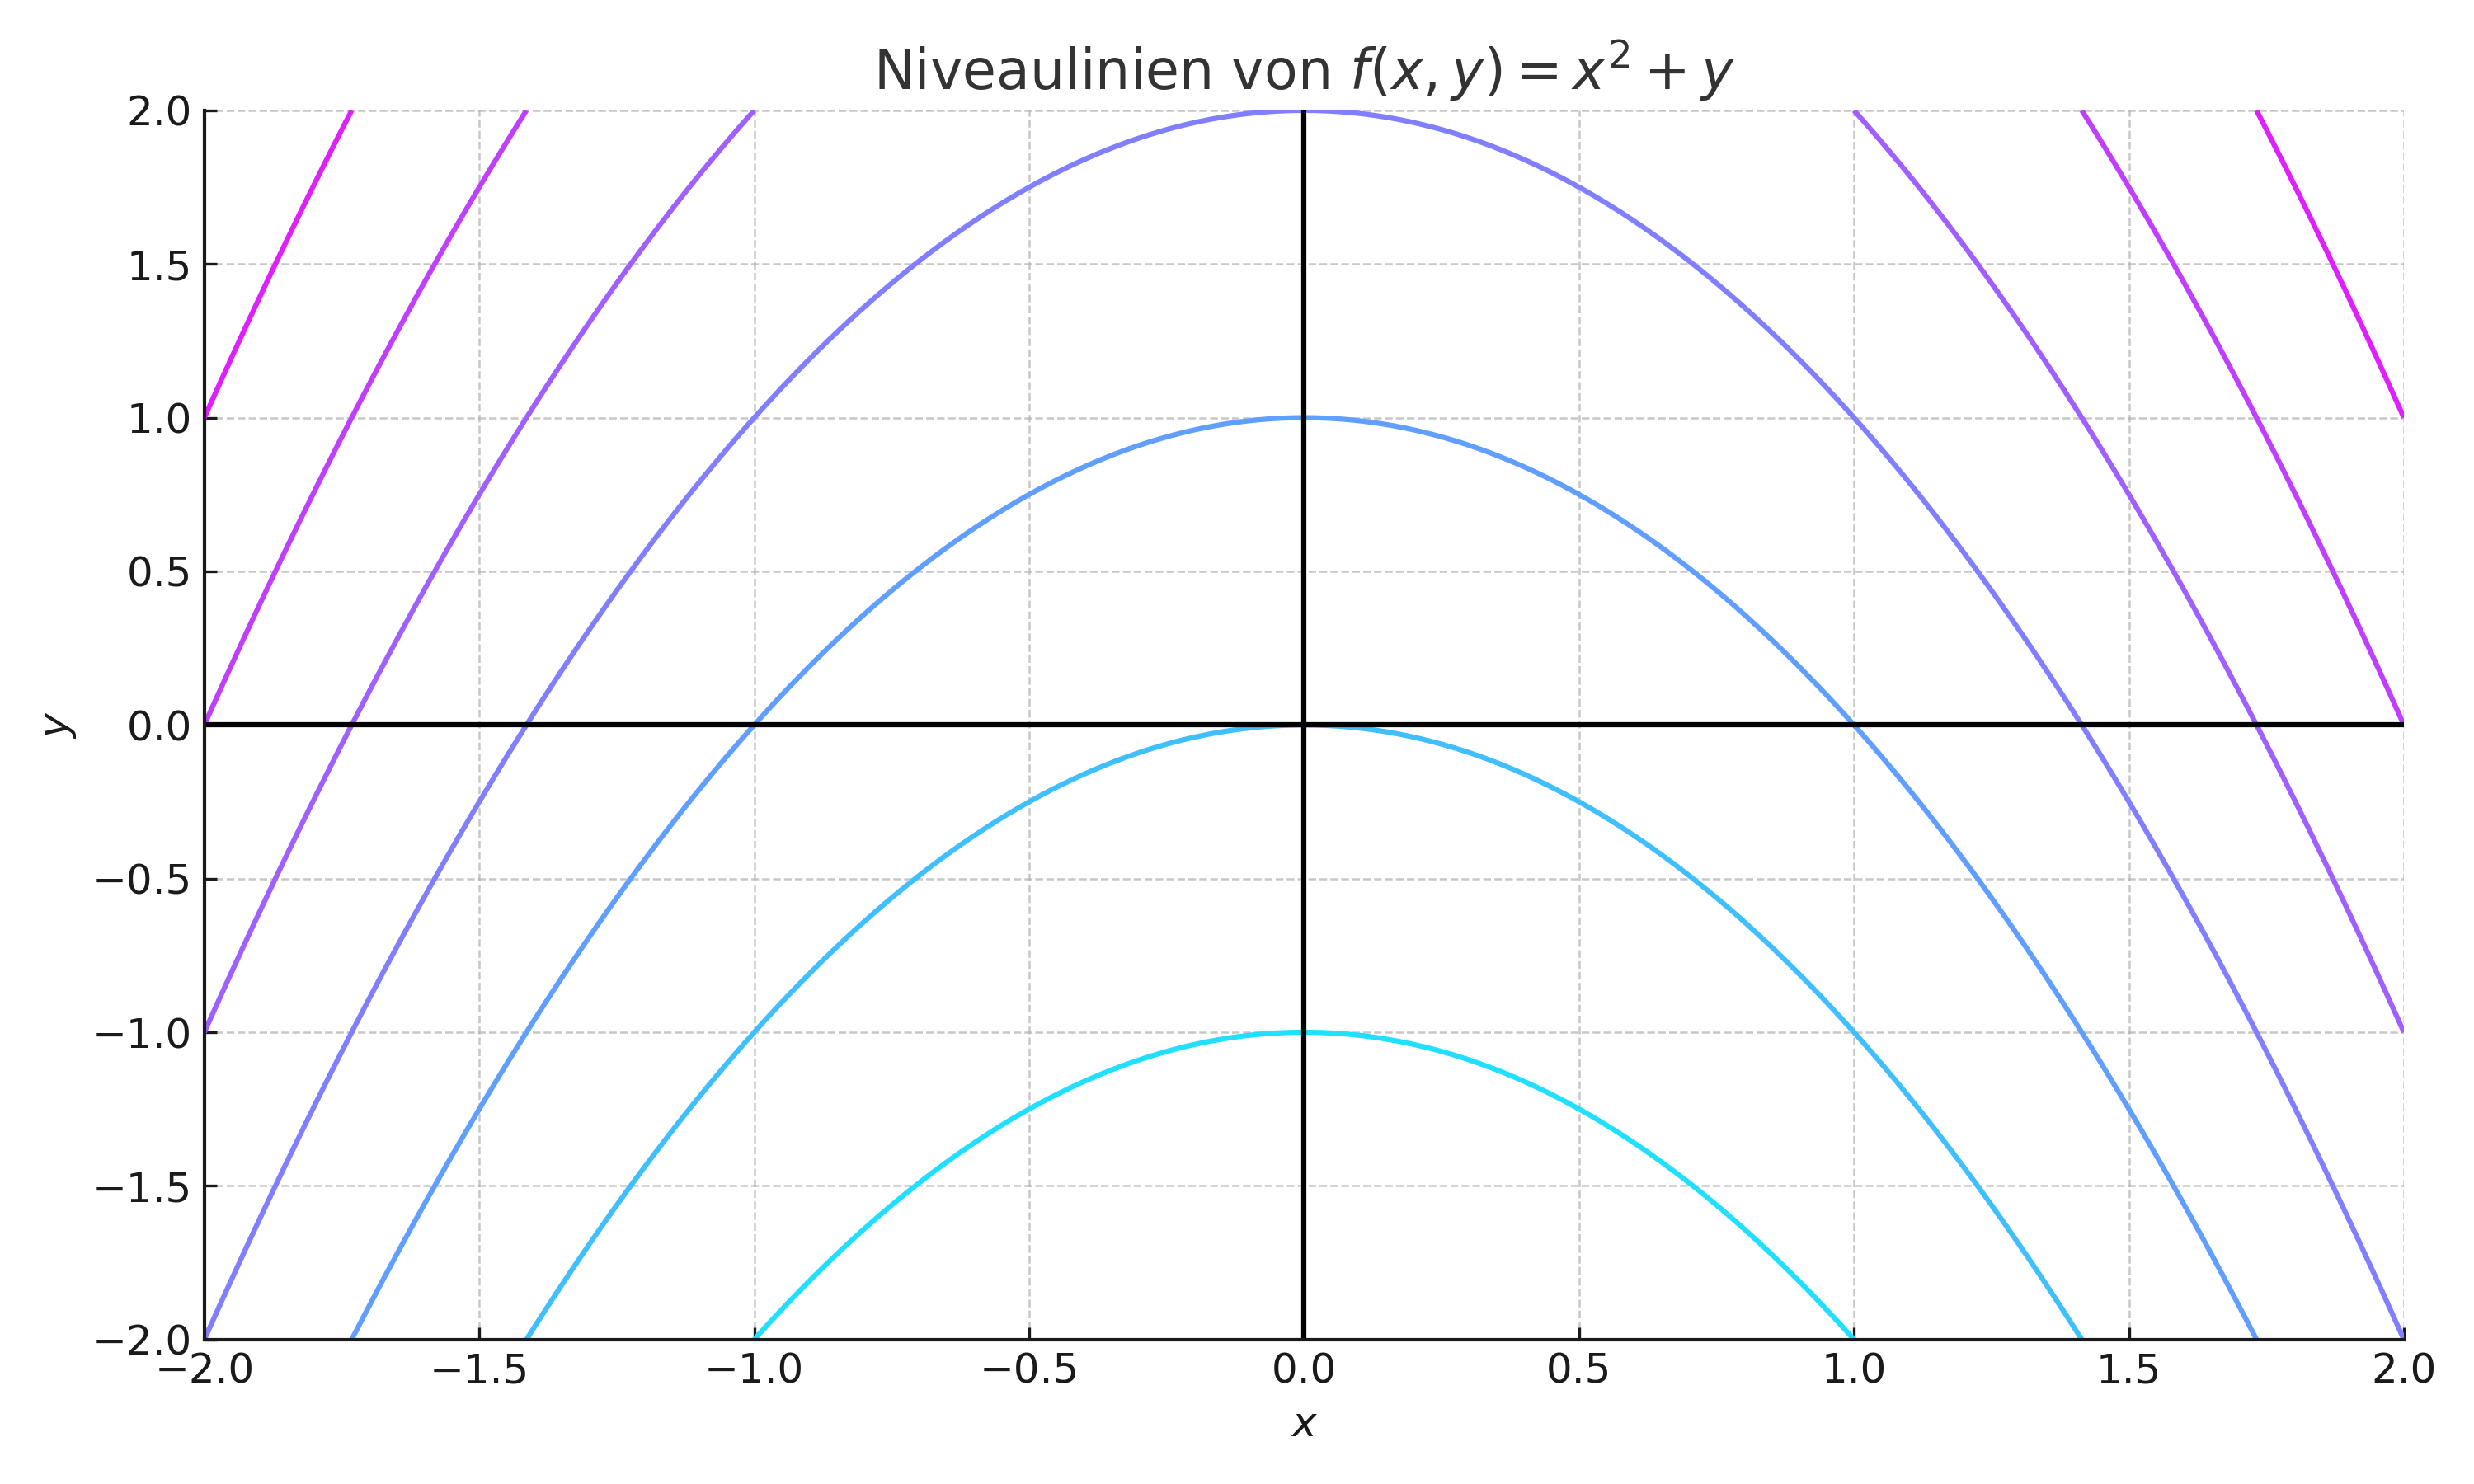
\includegraphics[width=\linewidth]{media/ueb1/niveau_f2_labeled.png}
			            %   \caption{Niveaulinien in der \( xy \)-Ebene}
			            % \end{subfigure}

			            % \vspace{1em}


		            \end{figure}
	      \end{enumerate}
	      \clearpage
	\item Niveaulinien
	      \begin{enumerate}
		      \item

		            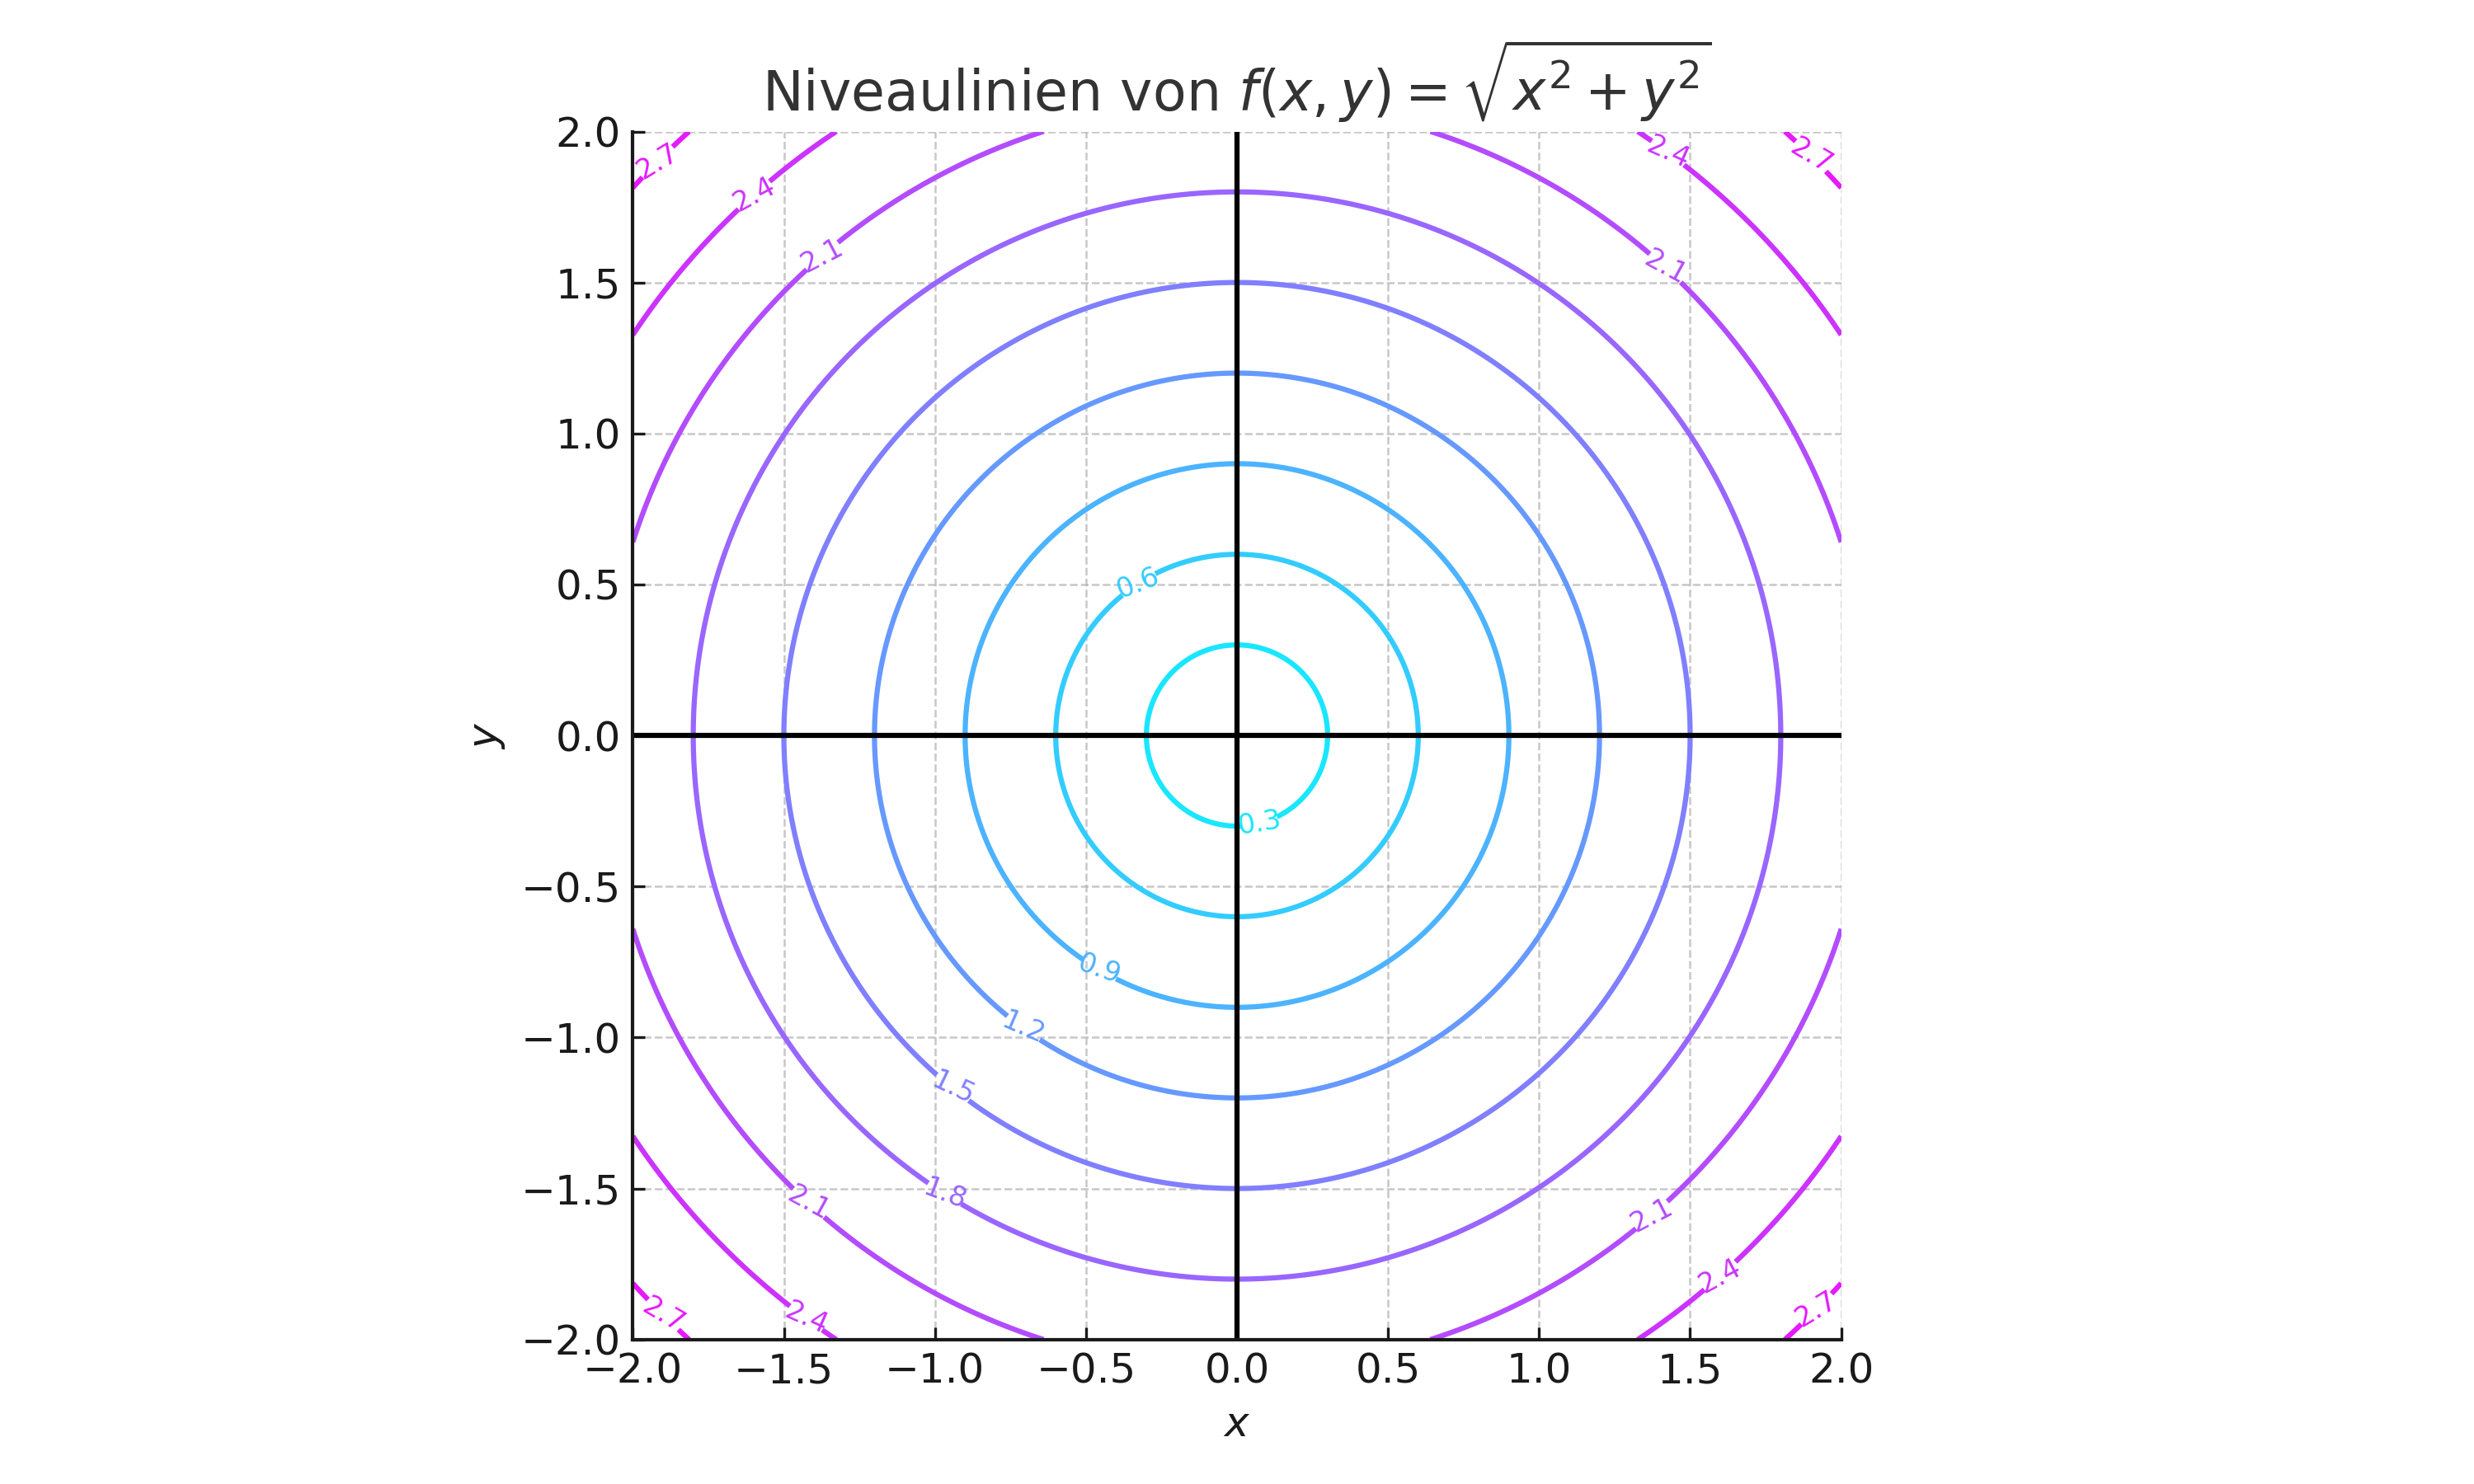
\includegraphics[width = 0.5\textwidth]{media/ueb1/niveau_g2_sqrt_contour.png}
		      \item

		            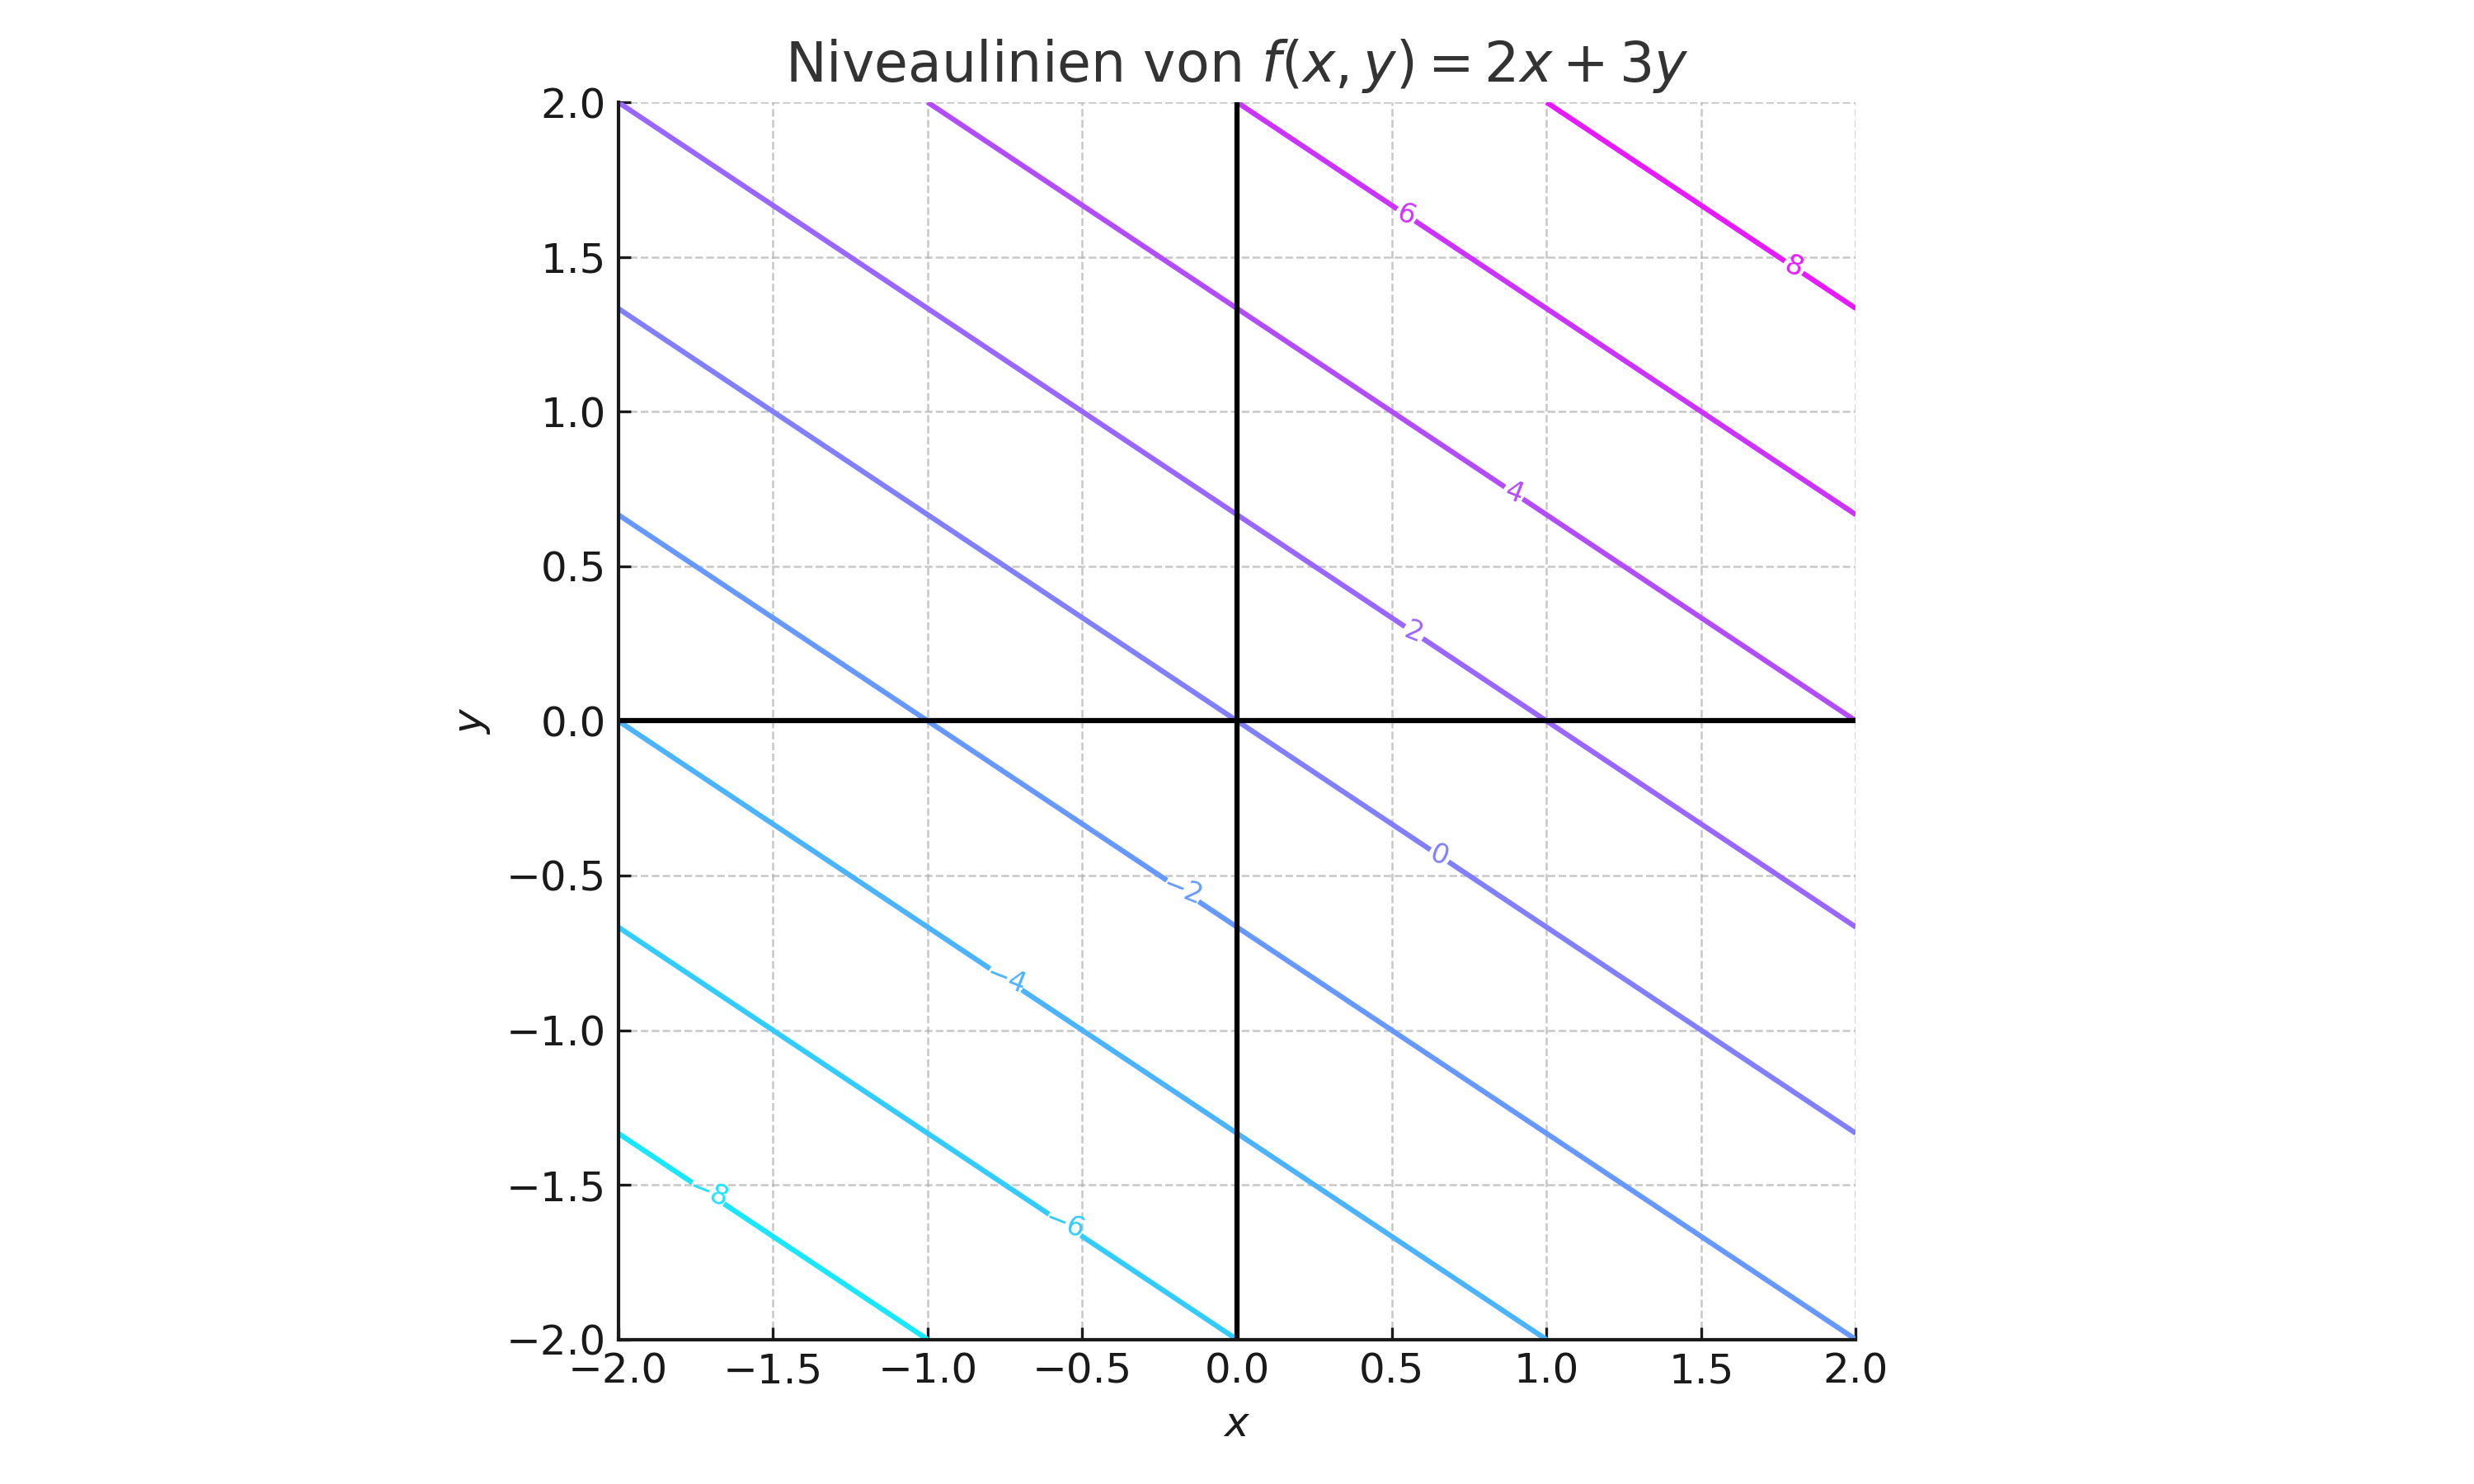
\includegraphics[width = 0.5\textwidth]{media/ueb1/niveau_g3_linear_contour.png}
		      \item

		            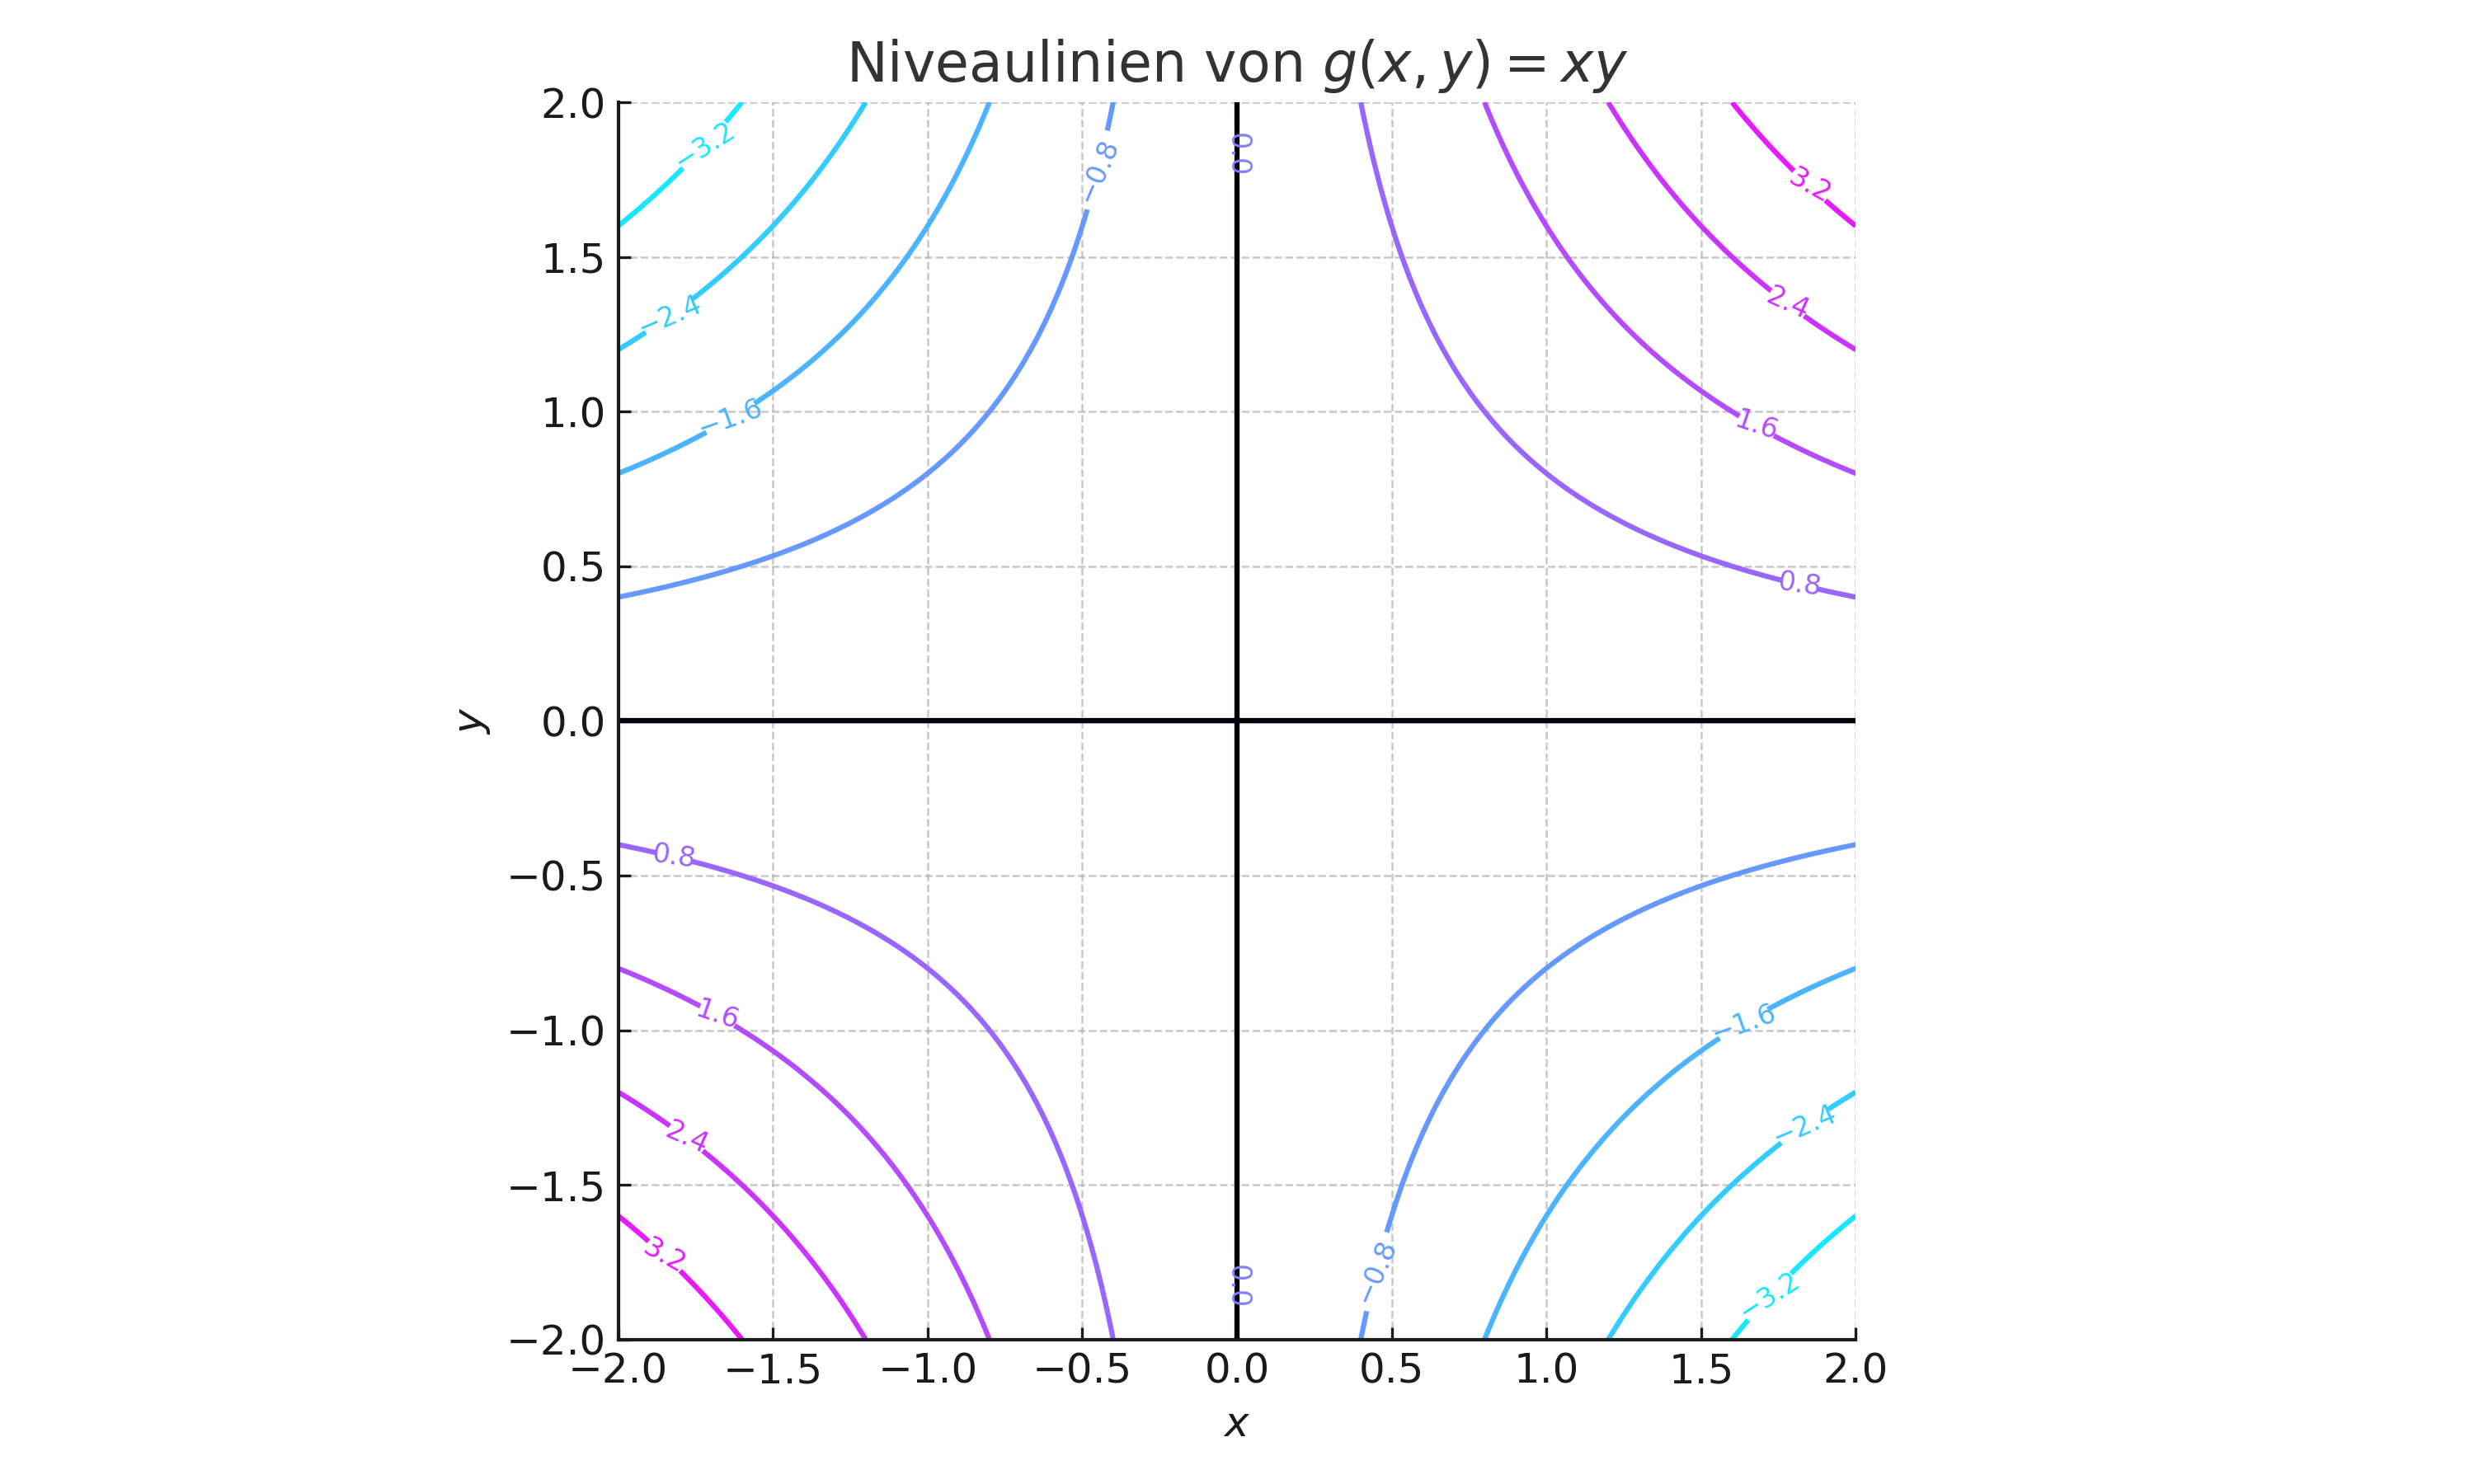
\includegraphics[width = 0.5\textwidth]{media/ueb1/niveau_g1_xy_contour.png}
	      \end{enumerate}
\end{enumerate}
\clearpage
\section{Partielle Ableitung}
\subsection*{Ableitung: Rückblick und Erweiterung}

Wir erinnern zunächst an den Begriff der Ableitung bei einer Funktion in einer Variablen: Definitionsgemäss wird der Grenzwert
\[
	f'(x_0) = \lim_{h \to 0} \frac{f(x_0 + h) - f(x_0)}{h}
\]
als \textbf{erste Ableitung} der Funktion \( f \) an der Stelle \( x_0 \) bezeichnet.

Aus geometrischer Sicht lässt sich diese Ableitung als \textbf{Steigung der Kurventangente} im Punkt \( P(x_0, y_0) \) deuten.

\medskip

Betrachtet man nun eine Funktion \( f \colon \mathbb{R}^2 \to \mathbb{R} \), dann merkt man schnell, dass man die Idee der Ableitung als Steigung der Tangente nicht ohne Weiteres übernehmen kann. Im Gegensatz zum eindimensionalen Fall gibt es nun nämlich \textbf{unendlich viele Tangenten}, die durch einen gegebenen Punkt \( P = (x_0, y_0, f(x_0, y_0)) \) verlaufen.

% Betrachtet man nun eine Funktion \( f \colon \mathbb{R}^2 \to \mathbb{R} \), dann merkt man schnell, dass man die Definition für die Ableitung nicht ohne Weiteres übernehmen kann. Sowohl die formale Definition als auch die geometrische Interpretation lassen sich nicht direkt übertragen:

% \begin{itemize}
%   \item Die Inputs sind Vektoren. Der Ausdruck
%   \[
%   \lim_{\vec{h} \to 0} \frac{f((x_0, y_0) + \vec{h}) - f(x_0, y_0)}{\vec{h}}
%   \]
%   ist \textbf{nicht definiert}, da eine Division durch einen Vektor nicht sinnvoll ist.

%   \item Im Gegensatz zum eindimensionalen Fall gibt es nun \textbf{unendlich viele Tangenten}, die durch einen gegebenen Punkt \( P = (x_0, y_0, f(x_0, y_0)) \) verlaufen.
% \end{itemize}

Die Abbildung zeigt in \textcolor{red}{Rot} und in \textcolor{blue}{Blau} die Tangenten in die Koordinatenrichtungen sowie in \textcolor{black}{Schwarz} die Tangente in Richtung der ersten Winkelhalbierenden dieser Koordinatenrichtungen.
\begin{center}
	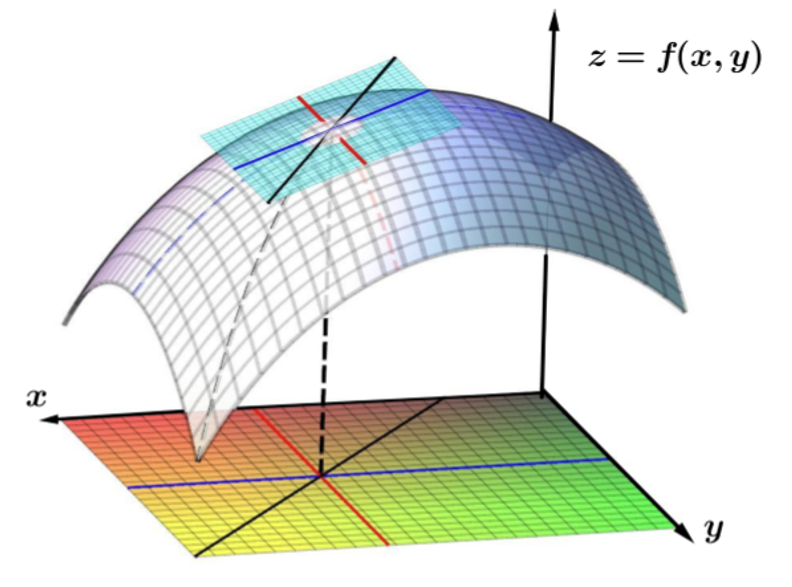
\includegraphics[width = 0.5 \textwidth]{media/GraphTangentialebene.png}
\end{center}

Die Steigung wird im Allgemeinen in verschiedenen Richtungen unterschiedlich sein. Man erhält also für jede Richtung eine eigene Ableitung!

















\subsection{Partielle Ableitungen in Koordinatenrichtungen}

Wir betrachten zuerst die Ableitungen in Richtung der Koordinatenachsen.


Der Graph der Funktion
\[
	f(x, y) = 1 - 3x^2 - y^2 + 5 \cdot \sin(xy)
\]
ist unten dargestellt.

Stellen Sie sich den Graphen der Funktion \( f \) als ein Gelände über der \( (x, y) \)-Ebene vor. Ein Wanderer befindet sich im Punkt
\[
	P = (1, 1, f(1, 1))
\]
und läuft in der gezeichneten Richtung, also \textbf{parallel zur \( xz \)-Ebene} (d.\,h. \( y = \text{konstant} \)).

\begin{center}
	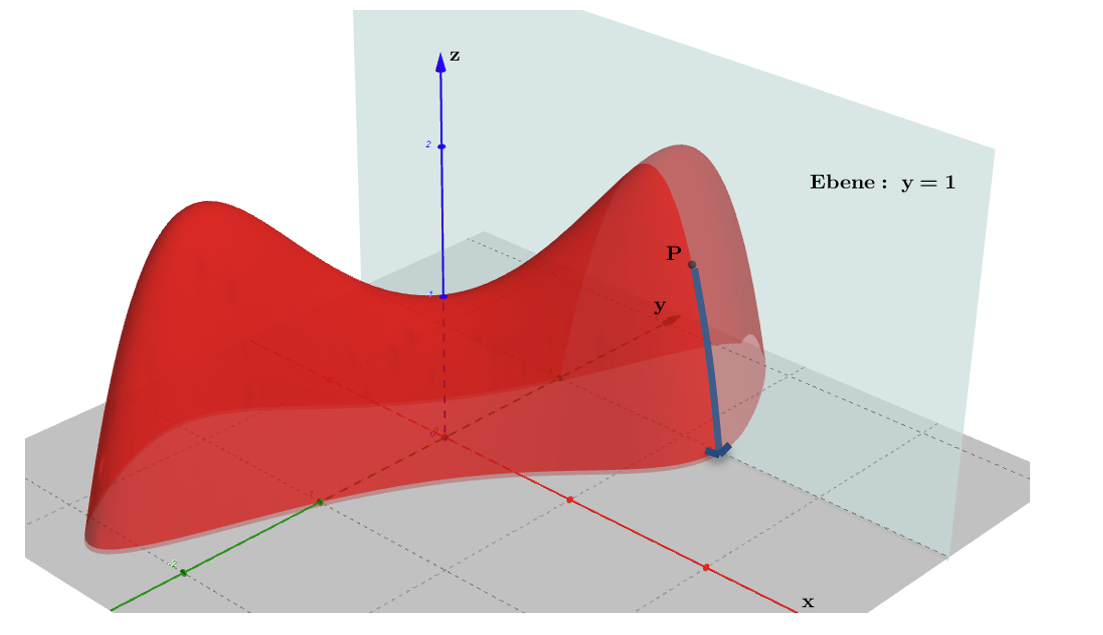
\includegraphics[width = 0.5\textwidth]{media/IntroPartielleAbleitung.png}
\end{center}

Wie steil ist sein Weg?

\medskip

Der Weg, dem der Wanderer folgt, entspricht dem Graphen der \textbf{partiellen Abbildung}
\[
	F_1(x) = f(x, 1)
	= 1 - 3x^2 - 1 + 5 \cdot \sin(x)
	= 5 \cdot \sin(x) - 3x^2
\]

\begin{center}
	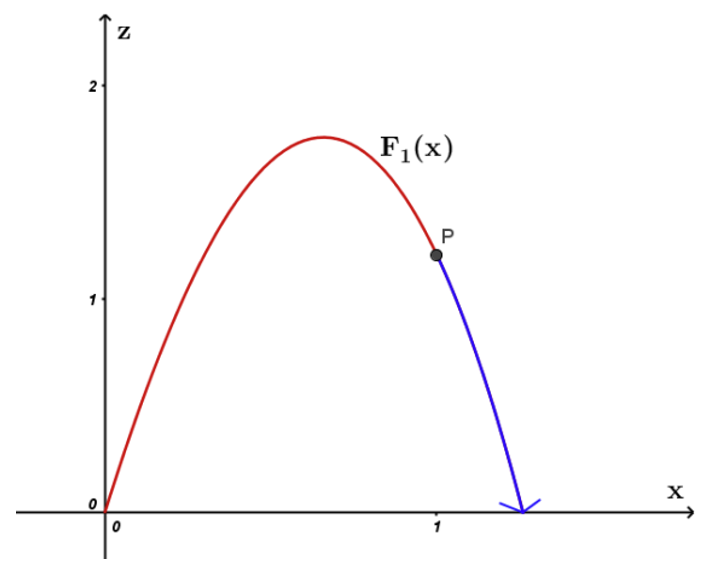
\includegraphics[width = 0.5\textwidth]{media/IntroPartielleAbleitung-Schnittkurve.png}
\end{center}



Die gesuchte Steigung ist nun die Steigung der Tangente an den Graphen von \( F_1 \) an der Stelle \( x = 1 \). Diese ist gleich der Ableitung:

\[
	F_1'(x) = 5 \cdot \cos(x) - 6x
	\quad \Rightarrow \quad
	F_1'(1) = 5 \cdot \cos(1) - 6 \approx -3.3
\]



Ein anderer Wanderer befindet sich im Punkt \( P = (x_0, y_0, f(x_0, y_0)) \) und läuft in dieselbe Richtung, also \textbf{in positive \( x \)-Richtung}. Wie steil ist sein Weg?

Die partielle Abbildung für festes \( y = y_0 \) lautet:
\[
	F_{y_0}(x) = f(x, y_0)
	= 1 - 3x^2 - y_0^2 + 5 \cdot \sin(x y_0)
\]

Die Steigung ergibt sich durch die Ableitung:
\[
	F_{y_0}'(x) = 5 \cdot \cos(x y_0) \cdot y_0 - 6x
	\quad \Rightarrow \quad
	F_{y_0}'(x_0) = 5 \cdot \cos(x_0 y_0) \cdot y_0 - 6x_0
\]

Diese Grösse nennt man die \textbf{partielle Ableitung} von \( f \) nach \( x \) an der Stelle \( (x_0, y_0) \).

\begin{definition}
	{Partielle Ableitung}{}
	Sei \( f \colon \mathbb{R}^2 \to \mathbb{R} \) eine Funktion und sei \( (x_0, y_0) \) eine Stelle im Definitionsbereich von \( f \).

	Falls die partiellen Abbildungen
	\[
		F_{y_0}(x) = f(x, y_0) \quad \text{bzw.} \quad F_{x_0}(y) = f(x_0, y)
	\]
	differenzierbar sind, so nennt man ihre Ableitungen die \textbf{partiellen Ableitungen} von \( f \) an der Stelle \( (x_0, y_0) \).

	Man bezeichnet sie durch die Symbole
	\[
		%f_x(x_0, y_0) \quad \text{oder} \quad 
		\frac{\partial f}{\partial x}(x_0, y_0) \qquad \text{bzw.} \qquad
		%f_y(x_0, y_0) \quad \text{oder} \quad 
		\frac{\partial f}{\partial y}(x_0, y_0)
	\]

	Formal sind sie als Grenzwerte definiert:
	\[
		\frac{\partial f}{\partial x}(x_0, y_0) = \lim_{\Delta x \to 0} \frac{f(x_0 + \Delta x, y_0) - f(x_0, y_0)}{\Delta x}
	\]
	\[
		\frac{\partial f}{\partial y}(x_0, y_0)= \lim_{\Delta y \to 0} \frac{f(x_0, y_0 + \Delta y) - f(x_0, y_0)}{\Delta y}
	\]

\end{definition}
Um die partielle Ableitung von \( f \) nach einer Variablen, z.\,B. nach \( x \), zu berechnen,
denkt man sich alle anderen Variablen als konstant und leitet dann mit den üblichen Differentiationsregeln nach \( x \) ab.


\begin{bsp}
	{}{}
	Gegeben sei die Funktion
	\[
		f(x, y) = e^{x^2 + 2y}
	\]

	\vspace*{3cm}

	% Für die partielle Ableitung nach \( x \) betrachtet man \( y \) als konstant und leitet mit der Kettenregel ab:
	% \[
	% \frac{\partial f}{\partial x}(x, y) = e^{x^2 + 2y} \cdot 2x
	% \]

	% Analog ergibt sich die partielle Ableitung nach \( y \):
	% \[
	% \frac{\partial f}{\partial y}(x, y) = e^{x^2 + 2y} \cdot 2
	% \]
\end{bsp}

\begin{bsp}
	{}{}
	Gegeben sei die Funktion
	\[
		f(x, y) = \sin\left(\frac{x}{y}\right)
	\]

	\vspace*{5cm}


	% Dann gilt:
	% \[
	% \frac{\partial f}{\partial x}(x, y) = \cos\left(\frac{x}{y}\right) \cdot \frac{1}{y}
	% \]

	% \[
	% \frac{\partial f}{\partial y}(x, y) = \cos\left(\frac{x}{y}\right) \cdot \left(-\frac{x}{y^2}\right)
	% \]
\end{bsp}

\begin{ueb}
	{}{}

	\begin{enumerate}
		\item Bestimmen Sie die partiellen Ableitungen der folgenden Funktionen:
		      \begin{enumerate}
			      \item \( f(x, y) = (x^2 - 1)(y + 2) \)
			      \item \( f(x, y) = (xy - 1)^2 \)
			      \item \( f(t, \alpha) = \cos(2\pi t - \alpha) \)
			      \item \( h(r, s) = \dfrac{2rs + r^2}{s + r} \)
			      \item \( g(a, b) = \ln(a) \cdot (2a - b) \)
		      \end{enumerate}

		\item Untersuchen Sie den Graphen von \( f(x, y) = (x^2 - 1)(y + 2) \) (siehe Aufgabe 1a) mit GeoGebra.
		      \begin{enumerate}
			      \item Es gilt: \( \frac{\partial f}{\partial x}(0, y) = 0 \). Woran erkennt man das im Graphen?
			      \item Es gilt: \( \frac{\partial f}{\partial x}(1, -2) = \frac{\partial f}{\partial y}(1, -2) = 0 \). Woran erkennt man das im Graphen?
		      \end{enumerate}

		\item Bestimmen Sie alle Funktionen \( f \), für die jeweils gilt:
		      \begin{enumerate}
			      \item \( \frac{\partial f}{\partial x}(x, y) = 0 \)
			      \item \( \frac{\partial f}{\partial x}(x, y) = \frac{\partial f}{\partial y}(x, y) = 0 \)
			      \item \( \frac{\partial f}{\partial y}(x, y) = x^2 \sin(xy) \)
		      \end{enumerate}
	\end{enumerate}
\end{ueb}
\clearpage
\emph{Lösungen:}


\begin{enumerate}
	\item Partielle Ableitungen:
	      \begin{enumerate}
		      \item Für \( f(x, y) = (x^2 - 1)(y + 2) \):
		            \[
			            \frac{\partial f}{\partial x}(x, y) = 2x(y + 2), \quad
			            \frac{\partial f}{\partial y}(x, y) = x^2 - 1
		            \]

		      \item Für \( f(x, y) = (xy - 1)^2 \):
		            \[
			            \frac{\partial f}{\partial x}(x, y) = 2(xy - 1)y, \quad
			            \frac{\partial f}{\partial y}(x, y) = 2(xy - 1)x
		            \]

		      \item Für \( f(t, \alpha) = \cos(2\pi t - \alpha) \):
		            \[
			            \frac{\partial f}{\partial t}(t, \alpha) = -\sin(2\pi t - \alpha) \cdot 2\pi, \quad
			            \frac{\partial f}{\partial \alpha}(t, \alpha) = \sin(2\pi t - \alpha)
		            \]

		      \item Für \( h(r, s) = \dfrac{2rs + r^2}{s + r} \):
		            \[
			            \frac{\partial h}{\partial r}(r, s) = \frac{2s^2 + r^2 + 2rs}{(s + r)^2}, \quad
			            \frac{\partial h}{\partial s}(r, s) = \frac{r^2}{(s + r)^2}
		            \]

		      \item Für \( g(a, b) = \ln(a) \cdot (2a - b) \):
		            \[
			            \frac{\partial g}{\partial a}(a, b) = 2\ln(a) + \frac{2a - b}{a}, \quad
			            \frac{\partial g}{\partial b}(a, b) = -\ln(a)
		            \]
	      \end{enumerate}
	\item \dots

	\item Allgemeine Lösungen:
	      \begin{enumerate}
		      \item Alle Funktionen, die unabhängig von \( x \) sind, also:
		            \[
			            f(x, y) = g(y)
		            \]

		      \item Alle konstanten Funktionen:
		            \[
			            f(x, y) = C, \quad \text{für ein } C \in \mathbb{R}
		            \]

		      \item Eine Funktion mit \( \frac{\partial f}{\partial y}(x, y) = x^2 \sin(xy) \) ist:
		            \[
			            f(x, y) = -x \cos(xy) + C
		            \]
	      \end{enumerate}
\end{enumerate}


























\subsection{Linearisierung und Tangentialebene}

Unter \emph{Linearisieren} versteht man die Approximation komplexer Funktionen durch eine lineare Funktion.

Das Linearisieren bei Funktionen zweier Variablen erfolgt vollkommen analog zum Linearisieren bei Funktionen einer Variablen.

Ist \( f \) eine Funktion einer Variablen, so approximiert man sie in der Nähe der Stelle \( x_0 \) durch die Tangente \( t(x) \), wobei die Gleichung der Tangente dem Taylorpolynom 1. Grades entspricht:
\[
	t(x) = f(x_0) + f'(x_0) \cdot (x - x_0)
\]

Ist \( f \) eine Funktion zweier Variablen, so linearisiert man diese an der Stelle \( (x_0, y_0) \), indem man sie durch diejenige lineare Funktion ersetzt, deren Graph gerade die Tangentialebene an den Graphen von \( f \) im Punkt
\[
	P = (x_0, y_0, f(x_0, y_0))
\]
ist.

Die Tangentialebene über der Stelle \( (x_0, y_0) \) besteht aus den Tangenten derjenigen Funktionen, die man durch Einschränkung von \( f \) entlang aller möglichen Geraden durch \( (x_0, y_0) \) erhält.

Die lineare Ersatzfunktion (deren Graph die Tangentialebene ist) besitzt folgende Eigenschaften:
\begin{itemize}
	\item ihr Wert in \( (x_0, y_0) \) ist \( f(x_0, y_0) \),
	\item ihre partielle Ableitung nach \( x \) ist \( \frac{\partial f}{\partial x} (x_0, y_0) \),
	\item ihre partielle Ableitung nach \( y \) ist \( \frac{\partial f}{\partial y} (x_0, y_0) \).
\end{itemize}

Diese drei Eigenschaften bestimmen die lineare Ersatzfunktion von \( f \) in \( (x_0, y_0) \) eindeutig. Sie ist gegeben durch:
\[
	T_{(x_0, y_0)}(x, y) = f(x_0, y_0) + \frac{\partial f}{\partial x} (x_0, y_0) \cdot (x - x_0) + \frac{\partial f}{\partial y} (x_0, y_0) \cdot (y - y_0)
\]

\begin{center}
	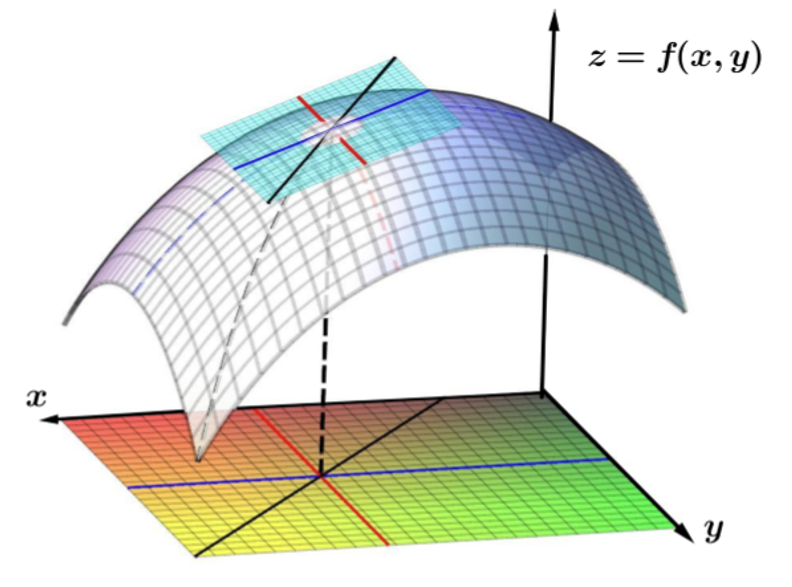
\includegraphics[width = 0.5 \textwidth]{media/GraphTangentialebene.png}
\end{center}

\begin{bsp}
	{Lineare Ersatzfunktion}{}


	Gegeben sei die Funktion
	\[
		f(x, y) = x^2 - y^2
	\]
	Gesucht ist die \textbf{lineare Ersatzfunktion} von \( f \) an der Stelle \( (1, -2) \). (Wird in der Klasse ergänzt.)

	% Die partiellen Ableitungen lauten:
	% \[
	% \frac{\partial f}{\partial x}(x, y) = 2x, \quad
	% \frac{\partial f}{\partial y}(x, y) = -2y
	% \]

	% Somit gilt:
	% \[
	% \frac{\partial f}{\partial x}(1, -2) = 2, \quad
	% \frac{\partial f}{\partial y}(1, -2) = 4
	% \]

	% Ausserdem berechnet man:
	% \[
	% f(1, -2) = 1^2 - (-2)^2 = 1 - 4 = -3
	% \]

	% Die lineare Ersatzfunktion \( T_{(1, -2)}(x, y) \) ist daher:
	% \[
	% T_{(1, -2)}(x, y) = -3 + 2(x - 1) + 4(y + 2) = 2x + 4y + 3
	% \]
	\vspace*{8cm}
\end{bsp}

\begin{ueb}
	{}{}

	\begin{enumerate}
		\item Bestimmen Sie die lineare Ersatzfunktion an der angegebenen Stelle.
		      Zeichnen Sie anschliessend den Graphen von \( f \) und jenen der Tangentialebene mit GeoGebra.
		      \begin{enumerate}
			      \item \( f(x, y) = \sqrt{x} + \sqrt{y} \), \quad \( P = (1, 1) \)
			      \item \( f(x, y) = \sqrt{xy - 1} \), \quad \( P = (5, 1) \)
			      \item \( f(x, y) = (x^2 - y^2) \cdot \sin(y) \), \quad \( P = (3, \frac{\pi}{2}) \)
		      \end{enumerate}

		\item Bestimmen Sie Näherungswerte für die folgenden Zahlen,
		      indem Sie die Funktion \( r(x, y) = \sqrt{x^2 + y^2} \) durch ihre lineare Ersatzfunktion an der Stelle \( P = (3, 4) \) approximieren:
		      \begin{enumerate}
			      \item \( \alpha = \sqrt{3.03^2 + 3.95^2} \)
			      \item \( \beta = \sqrt{2.94^2 + 4.07^2} \)
		      \end{enumerate}

		\item Geben Sie eine Gleichung der Tangentialebene an den Graphen von
		      \( f(x, y) = x^2 y^3 \) im Punkt \( P = (1 , -1) \) an.
		      Zeichnen Sie anschliessend den Graphen von \( f \) und die Tangentialebene mit GeoGebra.

		      % \item \textbf{Falls Sie die Ebenengleichung schon kennen:}  
		      % Geben Sie eine Formel für den Normalvektor der Tangentialebene an den Graphen der Funktion \( f(x, y) \) im Punkt \( P = (x_0, y_0) \) an.
	\end{enumerate}

\end{ueb}
\pagebreak
\emph{Lösungen}

\begin{enumerate}
	\item Lineare Ersatzfunktionen:
	      \begin{enumerate}
		      \item \( T_{(1,1)}(x, y) = \frac{1}{2}x + \frac{1}{2}y + 1 \)
		      \item \( T_{(5,1)}(x, y) = \frac{1}{4}x + \frac{5}{4}y - \frac{1}{2} \)
		      \item \( T_{\left(3, \frac{\pi}{2}\right)}(x, y) = 6x - \pi y + \frac{\pi^2}{4} - 9 \)
	      \end{enumerate}

	\item Näherung mit linearer Ersatzfunktion an \( P = (3,4) \) für \( r(x, y) = \sqrt{x^2 + y^2} \):
	      \[
		      T_{(3,4)}(x, y) = \frac{3}{5}x + \frac{4}{5}y
	      \]
	      \[
		      \alpha \approx 4.97, \quad \beta \approx 5.02
	      \]

	\item Tangentialebene:
	      \[
		      z = -2x + 3y + 4
	      \]

	      % \item Normalenvektor an den Graphen \( z = f(x, y) \) im Punkt \( (x_0, y_0) \):
	      % \[
	      % \vec{n} =
	      % \begin{pmatrix}
	      % f_x(x_0, y_0) \\
	      % f_y(x_0, y_0) \\
	      % -1
	      % \end{pmatrix}
	      % \]
\end{enumerate}















\clearpage
\subsection{Gradient und Richtungsableitung}
% \subsubsection*{Definition ACHTUNG: EHER WEGLASSEN (bereits halb begonnen ... )}

Genauso wie die Ableitungen in Richtung der Koordinatenachsen lassen sich natürlich auch die \emph{Richtungsableitungen} in beliebige andere Richtungen bilden.

% \begin{center}
%   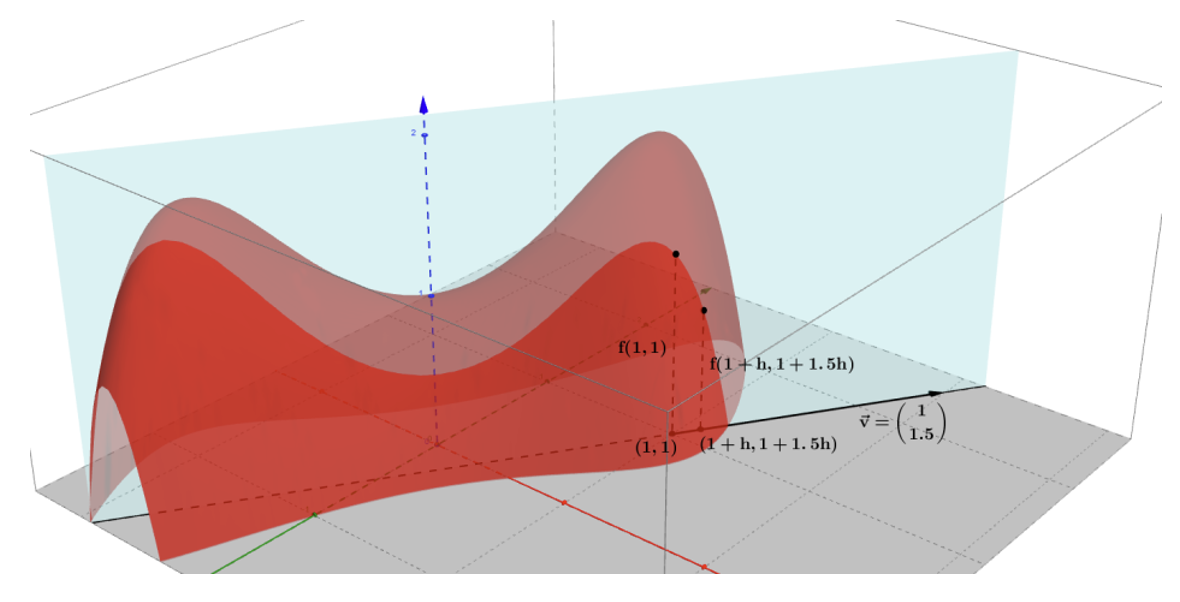
\includegraphics[width = \textwidth]{media/IntroRichtungsableitung.png}
% \end{center}

% Betrachten wir erneut den Wanderer im Punkt \( P = (1, 1) \). Diesmal läuft er jedoch in Richtung des Vektors
% \[
% \vec{v} = \begin{pmatrix} 1 \\ 1.5 \end{pmatrix}.
% \]

% Die Steigung des Weges in dieser Richtung ist gegeben durch den Grenzwert:
% \[
% \lim_{h \to 0} \frac{f(1 + h,\, 1 + 1.5h) - f(1, 1)}{\sqrt{h^2 + (1.5h)^2}}
% % =
% % \frac{1}{\sqrt{1^2 + (1.5)^2}}
% % \lim_{h \to 0} \frac{f(1 + h,\, 1 + 1.5h) - f(1, 1)}{h}
% =
% \frac{1}{|\vec{v}|}
% \lim_{h \to 0} \frac{f((1,\, 1) + h\cdot \vec{v} ) - f(1, 1)}{h}
% \]

% Dieser Ausdruck beschreibt die \textbf{Richtungsableitung} von \( f \) im Punkt \( (1, 1) \) in Richtung des Vektors \( \vec{v} \).

\begin{definition}
	{Richtungsableitung}{}

	Die Richtungsableitung einer Funktion \( f \) in Richtung eines Vektors $\vec{v}$
	% \[
	% \vec{v} = \begin{pmatrix} v_1 \\ v_2 \end{pmatrix}
	% \]
	an der Stelle \( P = (x_0, y_0) \) bezeichnet man mit
	\[ \frac{\partial f}{\partial \vec{v}}(x_0, y_0) \]
	% \[
	% \nabla_{\vec{v}} f(x_0, y_0).
	% \]
	% 

	Sie ist definiert durch den Grenzwert:
	\[
		%\nabla_{\vec{v}} f(x_0, y_0)
		\frac{\partial f}{\partial \vec{v}}(x_0, y_0)
		=
		\lim_{h \to 0}
		\frac{
			f((x_0 ,\, y_0) + h \vec{v}) - f(x_0, y_0)
			% =
			% \lim_{h \to 0}
			% \frac{
			% f(x_0 + h v_1,\, y_0 + h v_2) - f(x_0, y_0)
		}{
			h
		}
	\]

\end{definition}

\textbf{Bemerkungen:}
\begin{itemize}
	\item Die Richtungsableitung beschreibt die Steigung der Schnittkurve, die man erhält, wenn man den Graphen von \( f \) mit einer Ebene schneidet, die durch den Punkt \( P = (x_0, y_0, f(x_0, y_0)) \) verläuft und die Richtung des Vektors \( \vec{v} \) enthält.
	\item Man beachte jedoch, dass die horizontalen Änderung in Vielfache von $|\vec{v}|$ gemessen wird. Darum ist die Richtungsableitung vom Betrag des Vektors $\vec{v}$ abhängig. Die Richtungsableitung einer Funktion $f$ in Richtung des Vektors $2\cdot\vec{v}$ wird doppelt so gross sein, wie jene in Richtung des Vektors $\vec{v}$.
	\item Aus diesem Grund wird die Richtungsableitung häufig nur für normierte Vektoren, also für Vektoren der Länge Eins, betrachtet. In diesem Fall ist die Richtungsableitung tatsächlich eine Steigung.
	\item Die Richtungsableitung ist eine Verallgemeinerung der partiellen Ableitungen. Denn die Richtungsableitung in Richtung des Vektors \( \begin{pmatrix} 1 \\ 0 \end{pmatrix} \) entspricht der partiellen Ableitung nach \( x \), und die Richtungsableitung in Richtung des Vektors \( \begin{pmatrix} 0 \\ 1 \end{pmatrix} \) entspricht der partiellen Ableitung nach \( y \).
\end{itemize}






% \begin{satz}
% {Richtungsableitung und Steigung der Schnittkurve}{}
% Sei $f$ eine Funktion $f:\R^2\to\R^2$, $(x_0, y_0)\in \DD_f$  und $\vec{v} \in \R^2$. 

% \end{satz}

% \begin{bsp}
% 	{}{RichtungsableitungGrenzwert}
% 	Gegeben sei die Funktion
% 	\[
% 		f(x, y) = e^{xy}
% 	\]
% 	und der Punkt \( P = (1, 1) \). Gesucht ist die Richtungsableitung von \( f \) in Richtung des Vektors
% 	\[
% 		\vec{v} = \begin{pmatrix} 1 \\ 2 \end{pmatrix}.
% 	\]

% 	\vspace*{15cm}
% \end{bsp}

% \clearpage
\subsubsection*{Zusammenhang mit der partiellen Ableitung}
Die Ermittlung der Richtungsableitung mit dem Grenzwert kann sehr aufwendig sein. Abhilfe schafft eine geometrische Überlegung. Betrachten Sie die folgende Grafik
\begin{center}
	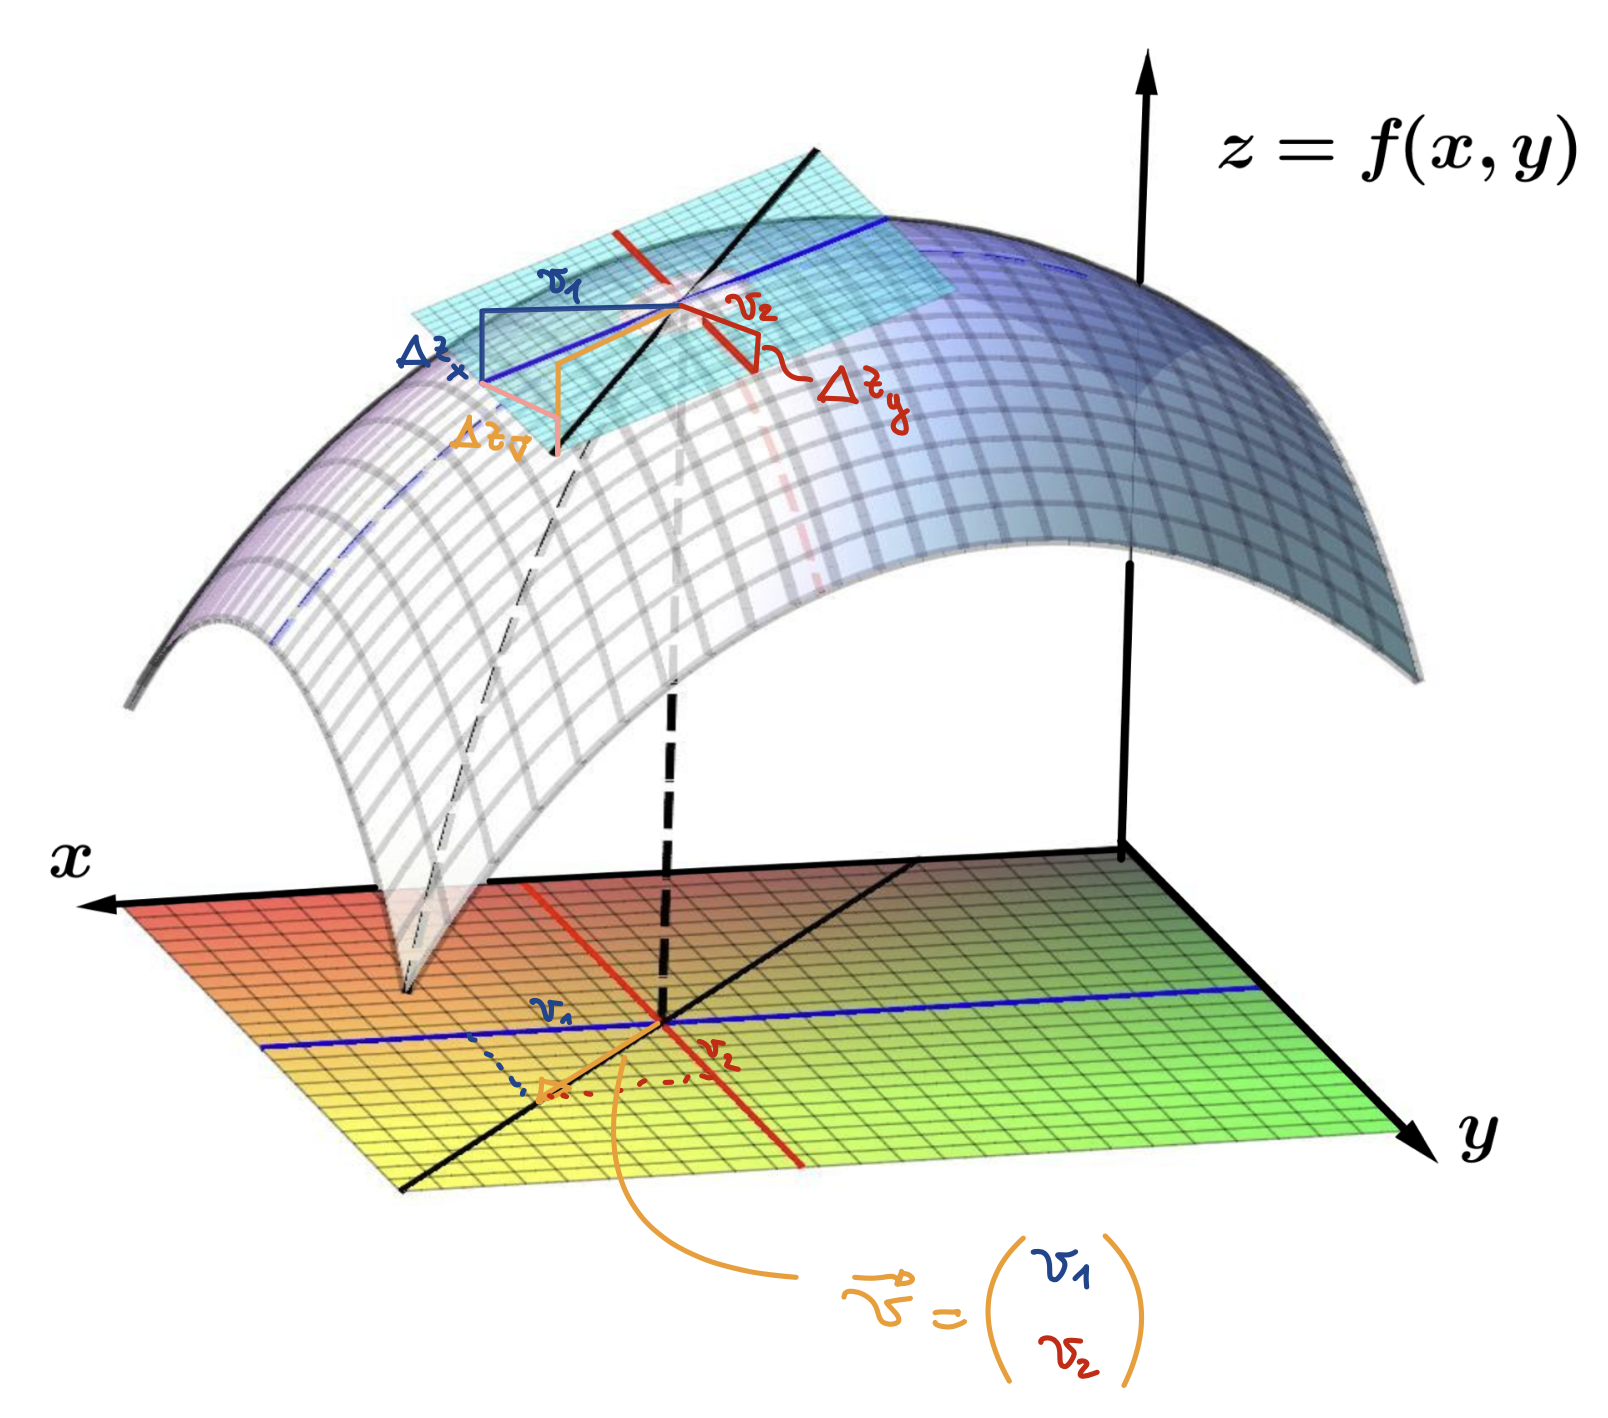
\includegraphics[width = \textwidth]{media/GradientundpartielleAbleitung.png}
\end{center}
Die Richtngsableitung $\frac{\partial f}{\partial \vec{v}}(x_0, y_0)$ ist die lokale Änderung der $z$-Koordinate, wenn man sich vom Punkt $(x_0, y_0)$ in Richtung des Vektors $\vec{v}$ bewegt. Mit den Bezeichnungen in der Grafik ist also:

\[
	%\nabla_{\vec{v}} f(x, y)
	\frac{\partial f}{\partial \vec{v}}(x_0, y_0)  = \Delta z_{\vec{v}}
\]

Für die Änderungen entlang der Koordinatenrichtungen gilt:

\[
	% \frac{\partial f}{\partial x}(x, y) = \frac{\Delta z_x}{v_1}
	% \quad \Rightarrow \quad
	\Delta z_x = v_1 \cdot \frac{\partial f}{\partial x}(x, y)
\]

\[
	% \frac{\partial f}{\partial y}(x, y) = \frac{\Delta z_y}{v_2}
	% \quad \Rightarrow \quad
	\Delta z_y = v_2 \cdot \frac{\partial f}{\partial y}(x, y)
\]

Offensichtlich gilt:
\[
	\Delta z_{\vec{v}} = \Delta z_x + \Delta z_y =
	v_1 \cdot \frac{\partial f}{\partial x}(x, y) +
	v_2 \cdot \frac{\partial f}{\partial y}(x, y)
\]

\begin{center}
	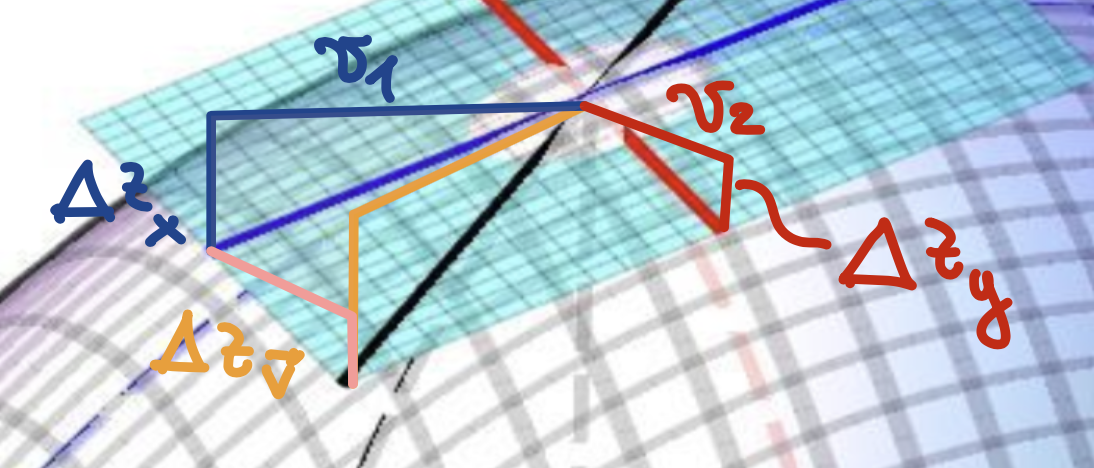
\includegraphics[width = \textwidth]{media/gradientundpartielleAbleitung2.png}
\end{center}

\begin{satz}
	{Richtungsableitung aus den partiellen Ableitungen}{}
	Es sei \( f \) eine stetig differenzierbare Funktion in zwei Variablen,
	sei \( (x_0, y_0) \) ein Punkt des Definitionsbereichs von \( f \),
	und sei
	\[
		\vec{v} = \begin{pmatrix} v_1 \\ v_2 \end{pmatrix}
	\]
	ein beliebiger Richtungsvektor.

	Dann gilt für die Richtungsableitung von \( f \) in Richtung \( \vec{v} \) an der Stelle \( (x_0, y_0) \):
	\[
		%\nabla_{\vec{v}} f(x_0, y_0) 
		\frac{\partial f}{\partial \vec{v}}(x_0, y_0) =
		v_1 \cdot \frac{\partial f}{\partial x}(x_0, y_0)
		+ v_2 \cdot \frac{\partial f}{\partial y}(x_0, y_0)
	\]
\end{satz}

Mit diesem Satz lässt sich die Richtungsableitung einfach berechnen.

\begin{bsp}
	{}{}
	% Vergleiche \Cref{bsp:RichtungsableitungGrenzwert}:
	Gegeben sei die Funktion
	\[
		f(x, y) = e^{xy}
	\]
	und der Punkt \( P = (1, 1) \). Gesucht ist die Richtungsableitung von \( f \) in Richtung des Vektors
	\[
		\vec{v} = \begin{pmatrix} 1 \\ 2 \end{pmatrix}.
	\]
	\vspace*{5cm}
\end{bsp}

\begin{ueb}
	{}{}


	\begin{enumerate}
		\item Berechnen Sie die Richtungsableitung der Funktion
		      \[
			      f(x, y) = 100xy
		      \]
		      in Richtung des Vektors
		      \[
			      \vec{v} = \begin{pmatrix} 1 \\ -1 \end{pmatrix}
		      \]
		      an der Stelle \( P = (x_0, y_0) \).

		\item \textbf{Kegel:}
		      \begin{enumerate}
			      \item

			            Berechnen Sie die Richtungsableitung der Funktion
			            \[
				            f(x, y) = \sqrt{x^2 + y^2}
			            \]
			            in Richtung des Vektors
			            \[
				            \vec{v} = \frac{1}{5} \begin{pmatrix} 4 \\ 3 \end{pmatrix}
			            \]
			            an der Stelle \( P = (x_0, y_0) \).



			      \item Liefern Sie eine \textbf{geometrische Erklärung} für die folgenden Aussagen zur Richtungsableitung aus Aufgabe (a).
			            (Es ist hilfreich, den Graphen mit GeoGebra darzustellen)

			            \begin{enumerate}
				            \item Die Richtungsableitung an der Stelle \( P = (0, 0) \) existiert nicht.
				            \item Die Richtungsableitung an der Stelle \( P = (4, 3) \) ist gleich Eins.
				            \item Die Richtungsableitung an der Stelle \( P = (-3, 4) \) ist gleich Null.
			            \end{enumerate}
		      \end{enumerate}
	\end{enumerate}

\end{ueb}

\clearpage
\emph{Lösungen}
\begin{enumerate}
	\item $100(y_0-x_0)$
	\item $\frac{4x_0+3y_0}{5\sqrt{x_0^2 + y_0^2}}$
\end{enumerate}




















\clearpage
\subsubsection*{Der Gradient}
Häufig wird der Term in der Formel für die Richtungsableitung als Skalarprodukt von zwei Vektoren interpretiert. Das Skalarprodukt wird im Grundlagenfach Mathematik behandeln. Für unsere Zwecke übernehmen wir ein paar Fakten, die im Grundlagenfach bewiesen werden.

Physikalische Grössen wie etwa Kraft, Geschwindigkeit oder Impuls beinhalten eine Richtung und werden mit Vektoren beschrieben, während Grössen wie Masse, Zeit oder Temperatur ungerichtet sind und sich durch eine einzige Zahl angeben lassen, die man in der Physik als Skalar bezeichnet.

\begin{definition}
	{Skalarprodukt}{}
	Seien $\vec{a}=\begin{pmatrix}
			a_1 \\a_2
		\end{pmatrix}$ und $\vec{b} = \begin{pmatrix}
			b_1 \\b_2
		\end{pmatrix}$ zwei Vektoren in $\R^2$. Dann ist das Skalarprodukt $\langle \vec{a}, \vec{b} \rangle$  definiert als
	$$ \langle \vec{a}, \vec{b} \rangle = a_1b_1 + a_2b_2$$
\end{definition}

\begin{bsp}
	{}{}
	$$\left\langle \begin{pmatrix} -2 \\ 3 \end{pmatrix}
		,
		\begin{pmatrix} 4 \\ 1 \end{pmatrix}
		\right\rangle
		= (-2) \cdot 4 + 3 \cdot 1
		= -8 + 3 = -5 $$
\end{bsp}

\textbf{Bemerkungen:}

\begin{itemize}
	\item Im Grundlagenfach bezeichnen wir das Skalarprodukt eher mit $\vec{a}\cdot \vec{b}$. Im Schwerpunktfach verwenden wir hingegen diese Notation, die auch an Hochschulen üblich ist.
	\item \( \vec{a} \) und \( \vec{b} \) sind Vektoren (sie haben eine Richtung),
	      \( \langle \vec{a}, \vec{b} \rangle \) ist ein \emph{Skalar} – also „bloss eine Zahl“.


	\item Seien \( \vec{a} \) und \( \vec{b} \) zwei Vektoren mit den Längen \( |\vec{a}| = 4 \) und \( |\vec{b}| = 3 \).
	      Je nach Zwischenwinkel \( \varepsilon \) variiert der Wert des Skalarprodukts \( \langle \vec{a}, \vec{b} \rangle \) wie folgt:

	      \begin{center}
		      \begin{tabular}{c|ccccccc}
			      \( \varepsilon \)                      & \( 0^\circ \) & \( 30^\circ \)  & \( 60^\circ \) & \( 90^\circ \) & \( 120^\circ \) & \( 150^\circ \)  & \( 180^\circ \) \\
			      \hline
			      \( \langle \vec{a}, \vec{b} \rangle \) & $12$          & \( 6\sqrt{3} \) & $6$            & $0$            & $-6$            & \( -6\sqrt{3} \) & $-12$
		      \end{tabular}
	      \end{center}



	      Der Wert des Skalarprodukts gibt also gewissermassen an, wie die beiden Vektoren zueinanderstehen.

\end{itemize}

Der Zusammenhang zwischen Skalarprodukt und gegenseitige Lage der Vektoren wird im Grundlagenfach genauer behandelt. Hier werden wir bloss zwei Fakten festhalten, die wir noch brauchen werden:
\clearpage
\begin{satz}
	{Skalarprodukt und gegenseitige Lage}{SkalarproduktundgegeseitigeLage}
	Für zwei Vektoren $\vec{a}$ und $\vec{b}$ gilt

	\begin{itemize}
		\item $ \vec{a}$ und $\vec{b}$ stehen genau dann senkrecht aufeinander, wenn deren Skalarprodukt $0$ ist:
		      $$ \vec{a} \perp \vec{b} \iff \langle\vec{a}, \vec{b} \rangle = 0$$
		\item Das Skalarprodukt von zwei Vektoren mit fester Länge ist genau dann maximal, wenn die Vektoren in die gleiche Richtung zeigen. In diesem Fall gilt
		      $$\vec{a} = \lambda\cdot \vec{b} \quad (\lambda >0)  \iff \langle\vec{a}, \vec{b} \rangle  = |\vec{a}| \cdot |\vec{b}|$$
	\end{itemize}

\end{satz}

\begin{bsp}
	{}{}
	\[
		\left\langle
		\begin{pmatrix} -2 \\ 3 \end{pmatrix},
		\begin{pmatrix} 6 \\ 4 \end{pmatrix}
		\right\rangle
		= (-2) \cdot 6 + 3 \cdot 4 = -12 + 12 = 0
	\]

	Die beiden Vektoren stehen  \textbf{senkrecht} aufeinander!

\end{bsp}

Mit dem Skalarprodukt lässt sich die Richtungsableitungen elegant berechnen. Es gilt nämlich:
\[
	%\nabla_{\vec{v}} f(x_0, y_0)
	\frac{\partial f}{\partial \vec{v}}(x_0, y_0)=
	v_1 \cdot \frac{\partial f}{\partial x}(x_0, y_0)
	+ v_2 \cdot \frac{\partial f}{\partial y}(x_0, y_0)
	= \left\langle \begin{pmatrix}
		\frac{\partial f}{\partial x}(x_0, y_0) \\
		\frac{\partial f}{\partial y}(x_0, y_0)
	\end{pmatrix}
	,
	\begin{pmatrix}
		v_1 \\v_2
	\end{pmatrix}
	\right\rangle
	=\langle \vec{\nabla} f(x_0, y_0), \vec{v} \rangle
\]

\begin{definition}
	{Der Gradient}{}
	Sei \( f \colon \mathbb{R}^2 \to \mathbb{R} \) eine Funktion mit der Eigenschaft, dass beide partiellen Ableitungen existieren.

	Der Gradient \( \vec{\nabla} f(x_0, y_0) \) von \( f \) im Punkt \( P = (x_0, y_0) \) ist der Vektor:
	\[
		\vec{\nabla} f(x_0, y_0) =
		\begin{pmatrix}
			\frac{\partial f}{\partial x}(x_0, y_0) \\
			\frac{\partial f}{\partial y}(x_0, y_0)
		\end{pmatrix}
	\]

\end{definition}

Mit dem Gradienten lässt sich die Richtungsableitung neu wie folgt berechnen:
\begin{satz}
	{Richtungsableitung als Skalarprodukt}{}

	Es sei \( f \) eine stetig differenzierbare Funktion in zwei Variablen und
	\( (x_0, y_0) \) ein Punkt des Definitionsbereiches von \( f \). Dann gilt:

	\[
		%\nabla_{\vec{v}} f(x_0, y_0)
		\frac{\partial f}{\partial \vec{v}}(x_0, y_0) = \left\langle \vec{\nabla} f(x_0, y_0),\, \vec{v} \right\rangle
	\]

	Dabei bezeichnet \( \langle \cdot, \cdot \rangle \) das \textbf{Skalarprodukt} der beiden Vektoren.

\end{satz}

Auf den ersten Blick hat man damit nicht viel gewonnen. Die Richtungsableitung wird immer noch genau gleich berechnet. Durch die Interpretation der Formel als Skalarprodukt können wir aber die geometrischen Eigenschaften des Skalarprodukt (also \Cref{satz:SkalarproduktundgegeseitigeLage}) auf die Richtungsableitung übertragen!

\begin{satz}
	{Eigenschaften des Gradienten}{}
	Für den Gradient$\vec{\nabla} f(x_0, y_0)$ einer Funktion $f$ an der Stelle $(x_0, y_0)$ gilt:
	\begin{itemize}
		\item $\vec{\nabla} f(x_0, y_0)$ steht senkrecht zur Niveaulinie von $f$ durch $(x_0, y_0)$.
		\item Die Richtung des Gradienten $\vec{\nabla} f(x_0, y_0)$ gibt die Richtung der grössten Richtungsableitung von $f$ in $(x_0,y_0)$ an (Richtung des maximalen Anstiegs des Graphen von $f$).
	\end{itemize}
\end{satz}

\begin{proof}
	\begin{itemize}
		\item Da sich der Funktionswert entlang der Niveaulinien nicht ändert, ist die Ableitung in Richtung der Tangente gleich null.

		      Das heisst: Ist \( \vec{v} \) ein Tangentenvektor an die Niveaulinie im Punkt \( (x_0, y_0) \), dann gilt:
		      \[
			      0 =
			      %\nabla_{\vec{v}} f(x_0, y_0)
			      \frac{\partial f}{\partial \vec{v}}(x_0, y_0)
			      = \left\langle \vec{\nabla} f(x_0, y_0),\, \vec{v} \right\rangle
		      \]
		      Aus \Cref{satz:SkalarproduktundgegeseitigeLage} folgt dann, dass die beiden Vektoren $\vec{\nabla} f(x_0, y_0)$ und  $\vec{v}$ senkrecht stehen. Fazit: Der Gradient steht stets senkrecht auf den Niveaulinien.
		      % \[
		      % \Longleftrightarrow \quad \left\langle \vec{\nabla} f(x_0, y_0),\, \vec{v} \right\rangle = 0
		      % \quad \Longleftrightarrow \quad \vec{v} \perp \vec{\nabla} f(x_0, y_0)
		      % \]
		\item Betrachten man alle Vektoren $\vec{v}$ in $\R^2$ dann ist die Richtungsableitung $\frac{\partial f}{\partial \vec{v}}(x_0, y_0)
			      = \left\langle \vec{\nabla} f(x_0, y_0),\, \vec{v} \right\rangle$ genau dann maximal, wenn $\vec{v} = \lambda  \vec{\nabla} f(x_0, y_0)$ (\Cref{satz:SkalarproduktundgegeseitigeLage}).

	\end{itemize}
\end{proof}

\noindent
\begin{minipage}[t]{0.48\textwidth}
	\centering
	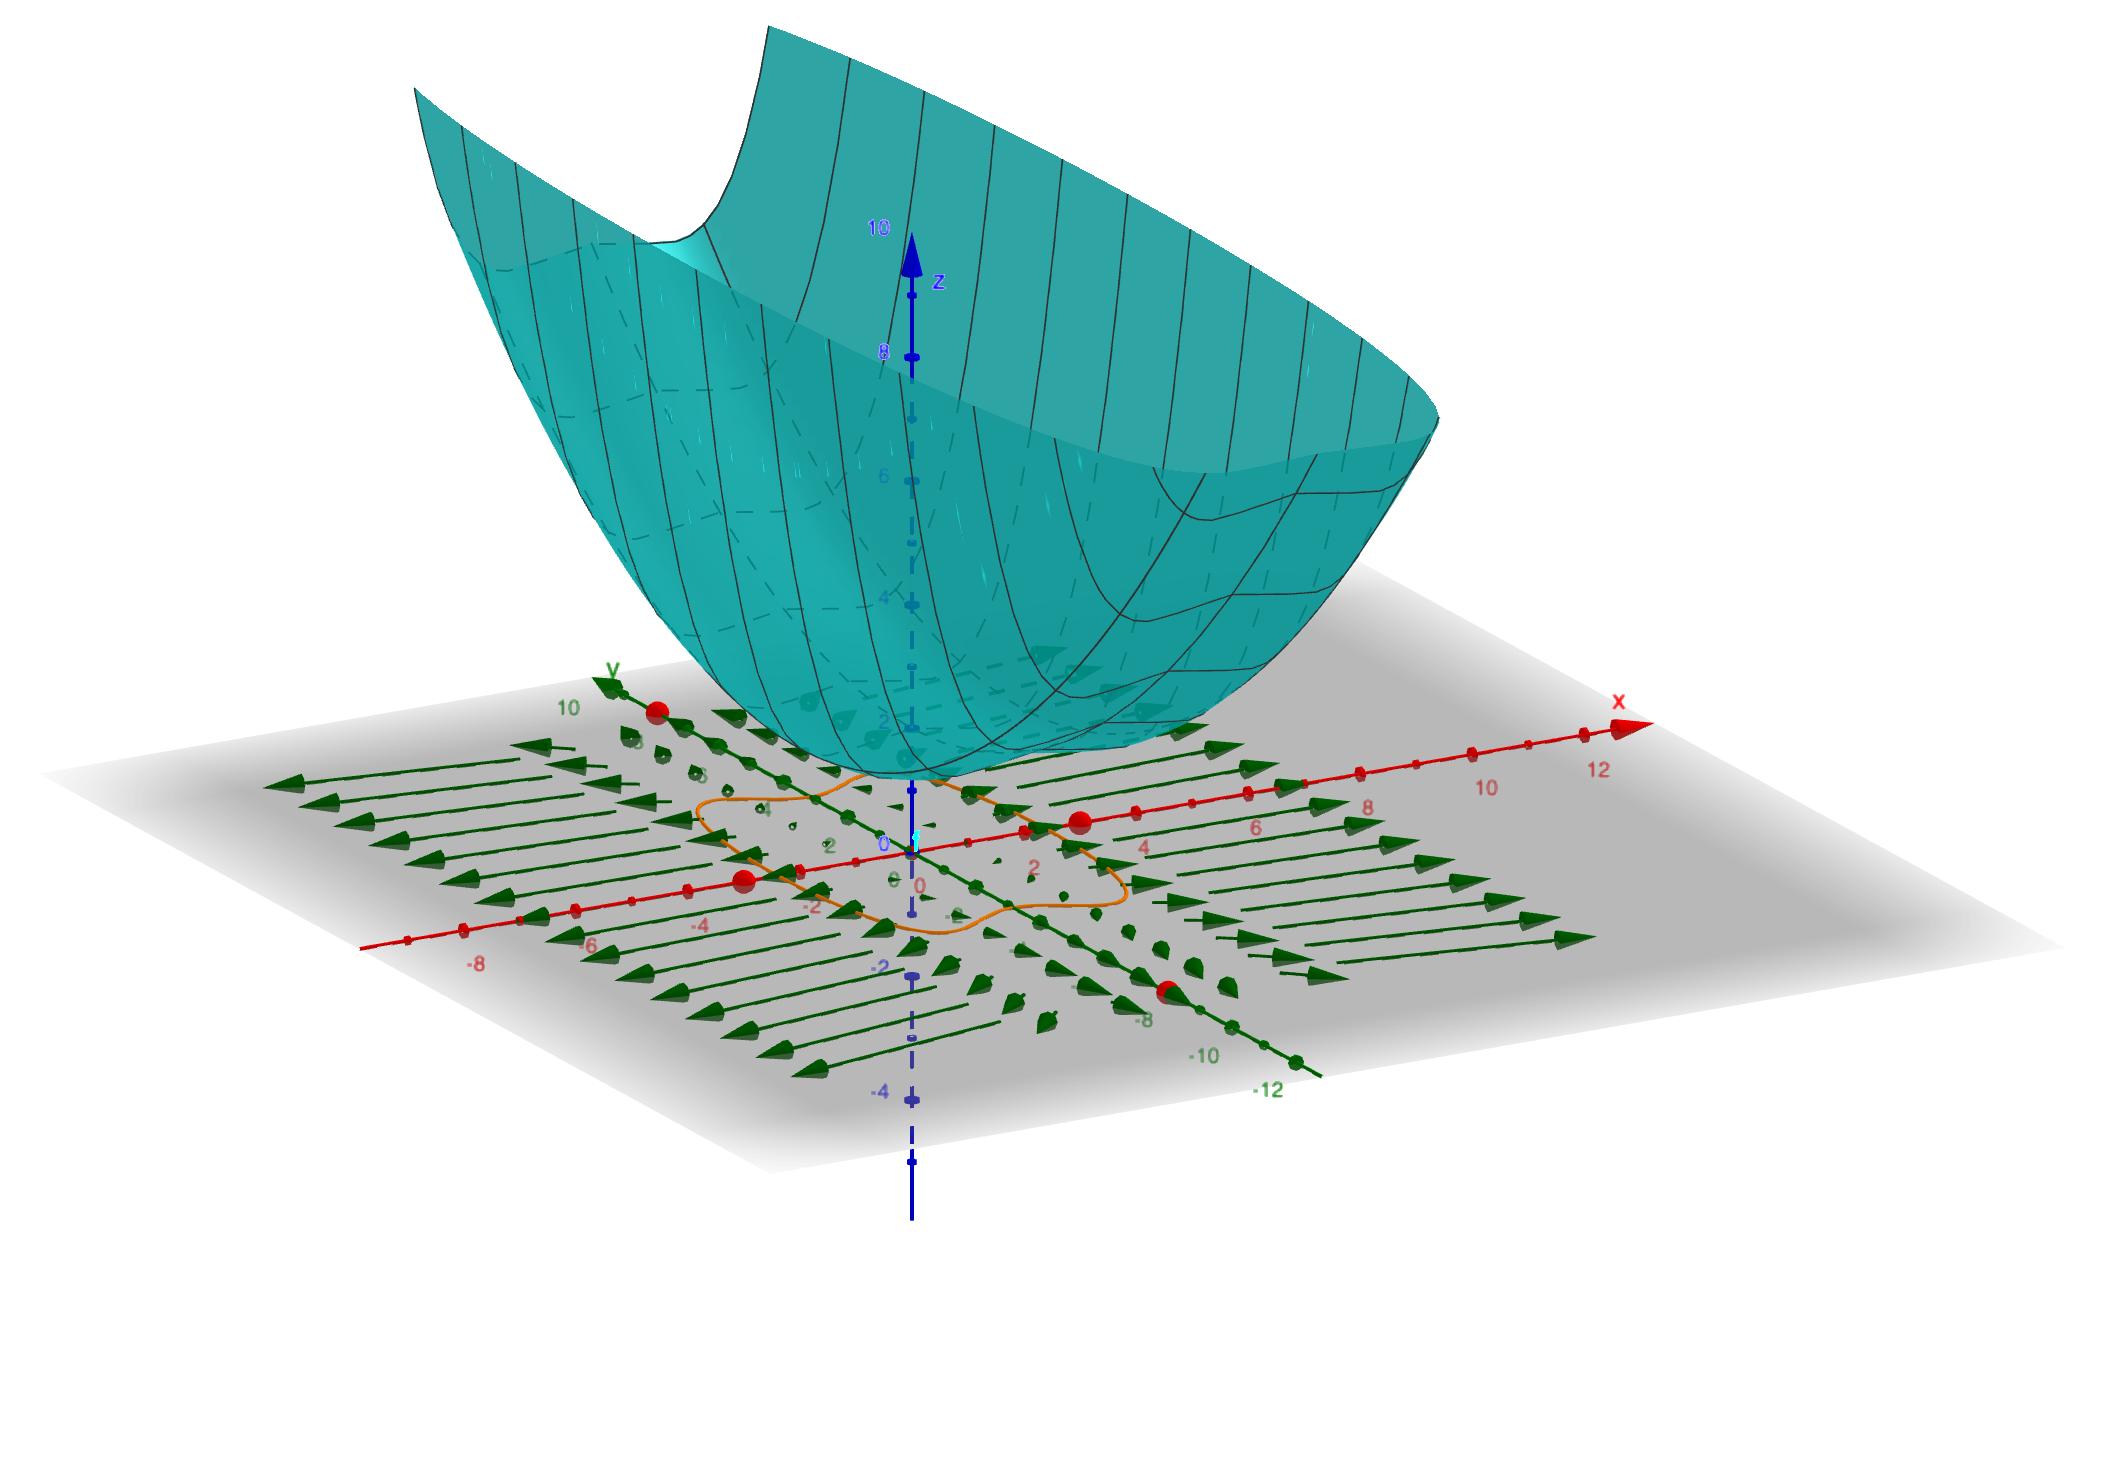
\includegraphics[width=\linewidth]{media/GradientenFeld.png}\\
	\small Graph einer Funktion $f$
\end{minipage}
\hfill
\begin{minipage}[t]{0.48\textwidth}
	\centering
	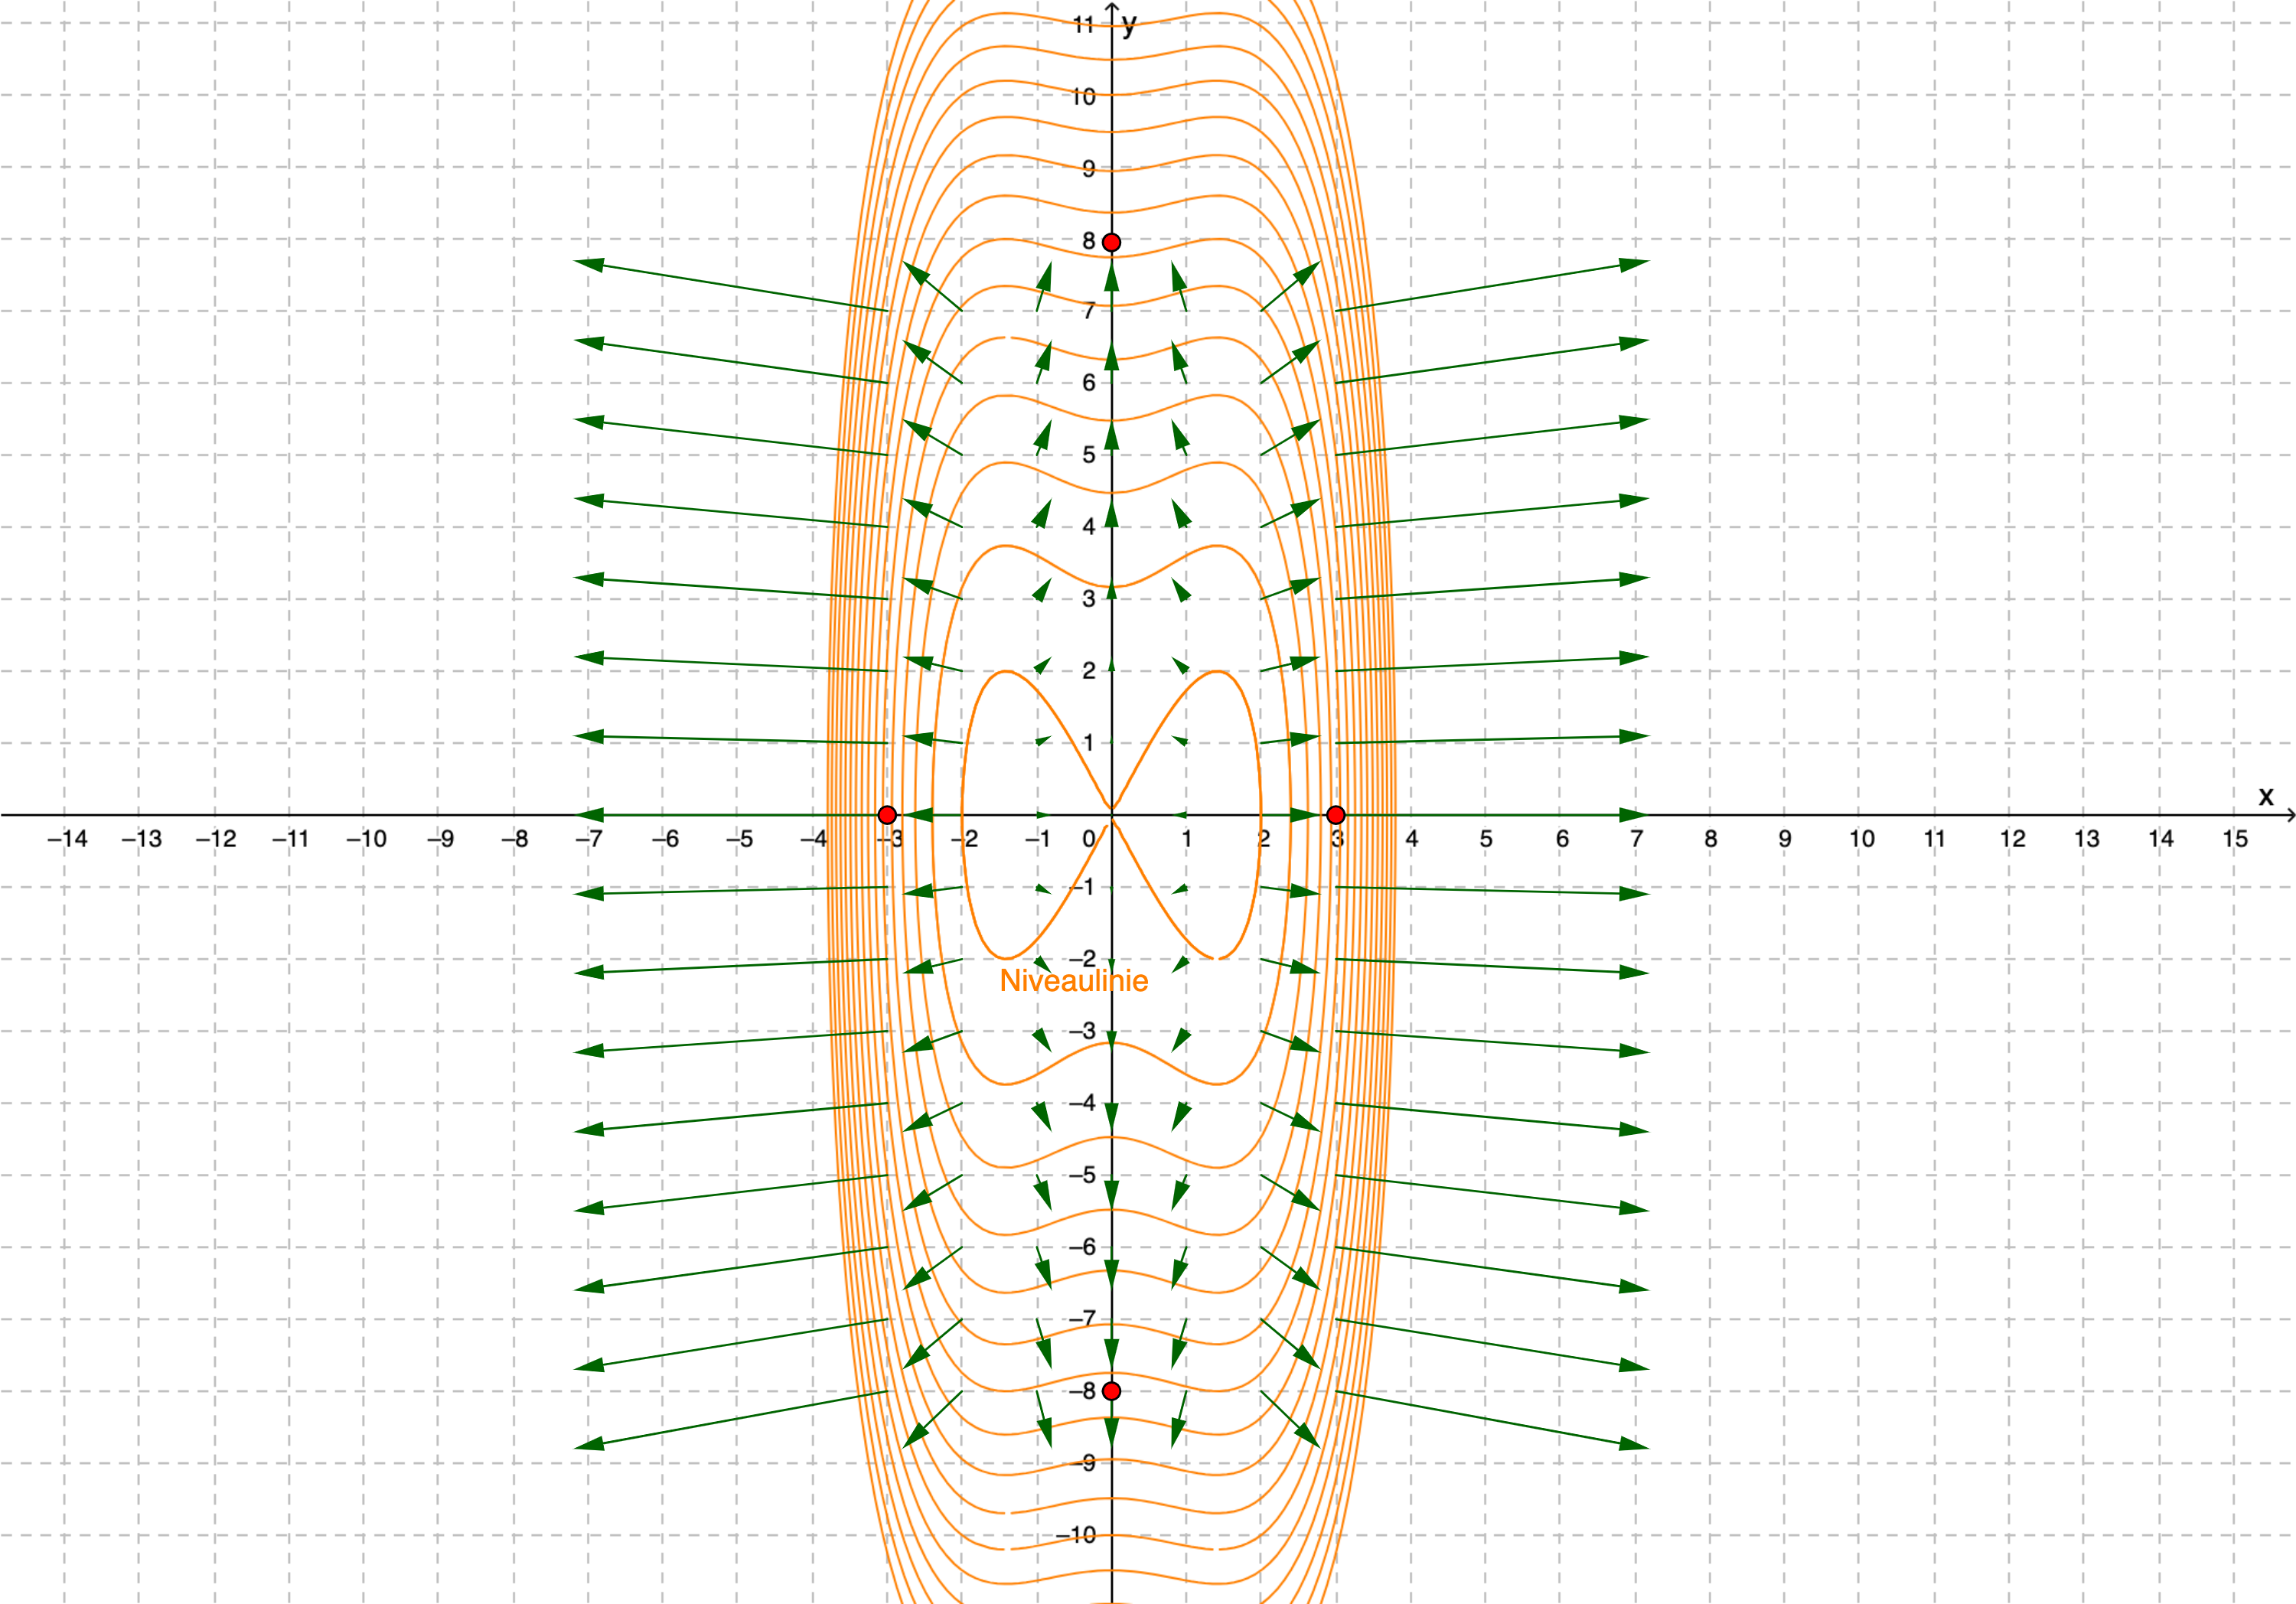
\includegraphics[width=\linewidth]{media/GradientNiveaulinie.png}\\
	\small Niveaulinien und Gradientenfeld der Funktion $f$
\end{minipage}

% \begin{center}
%   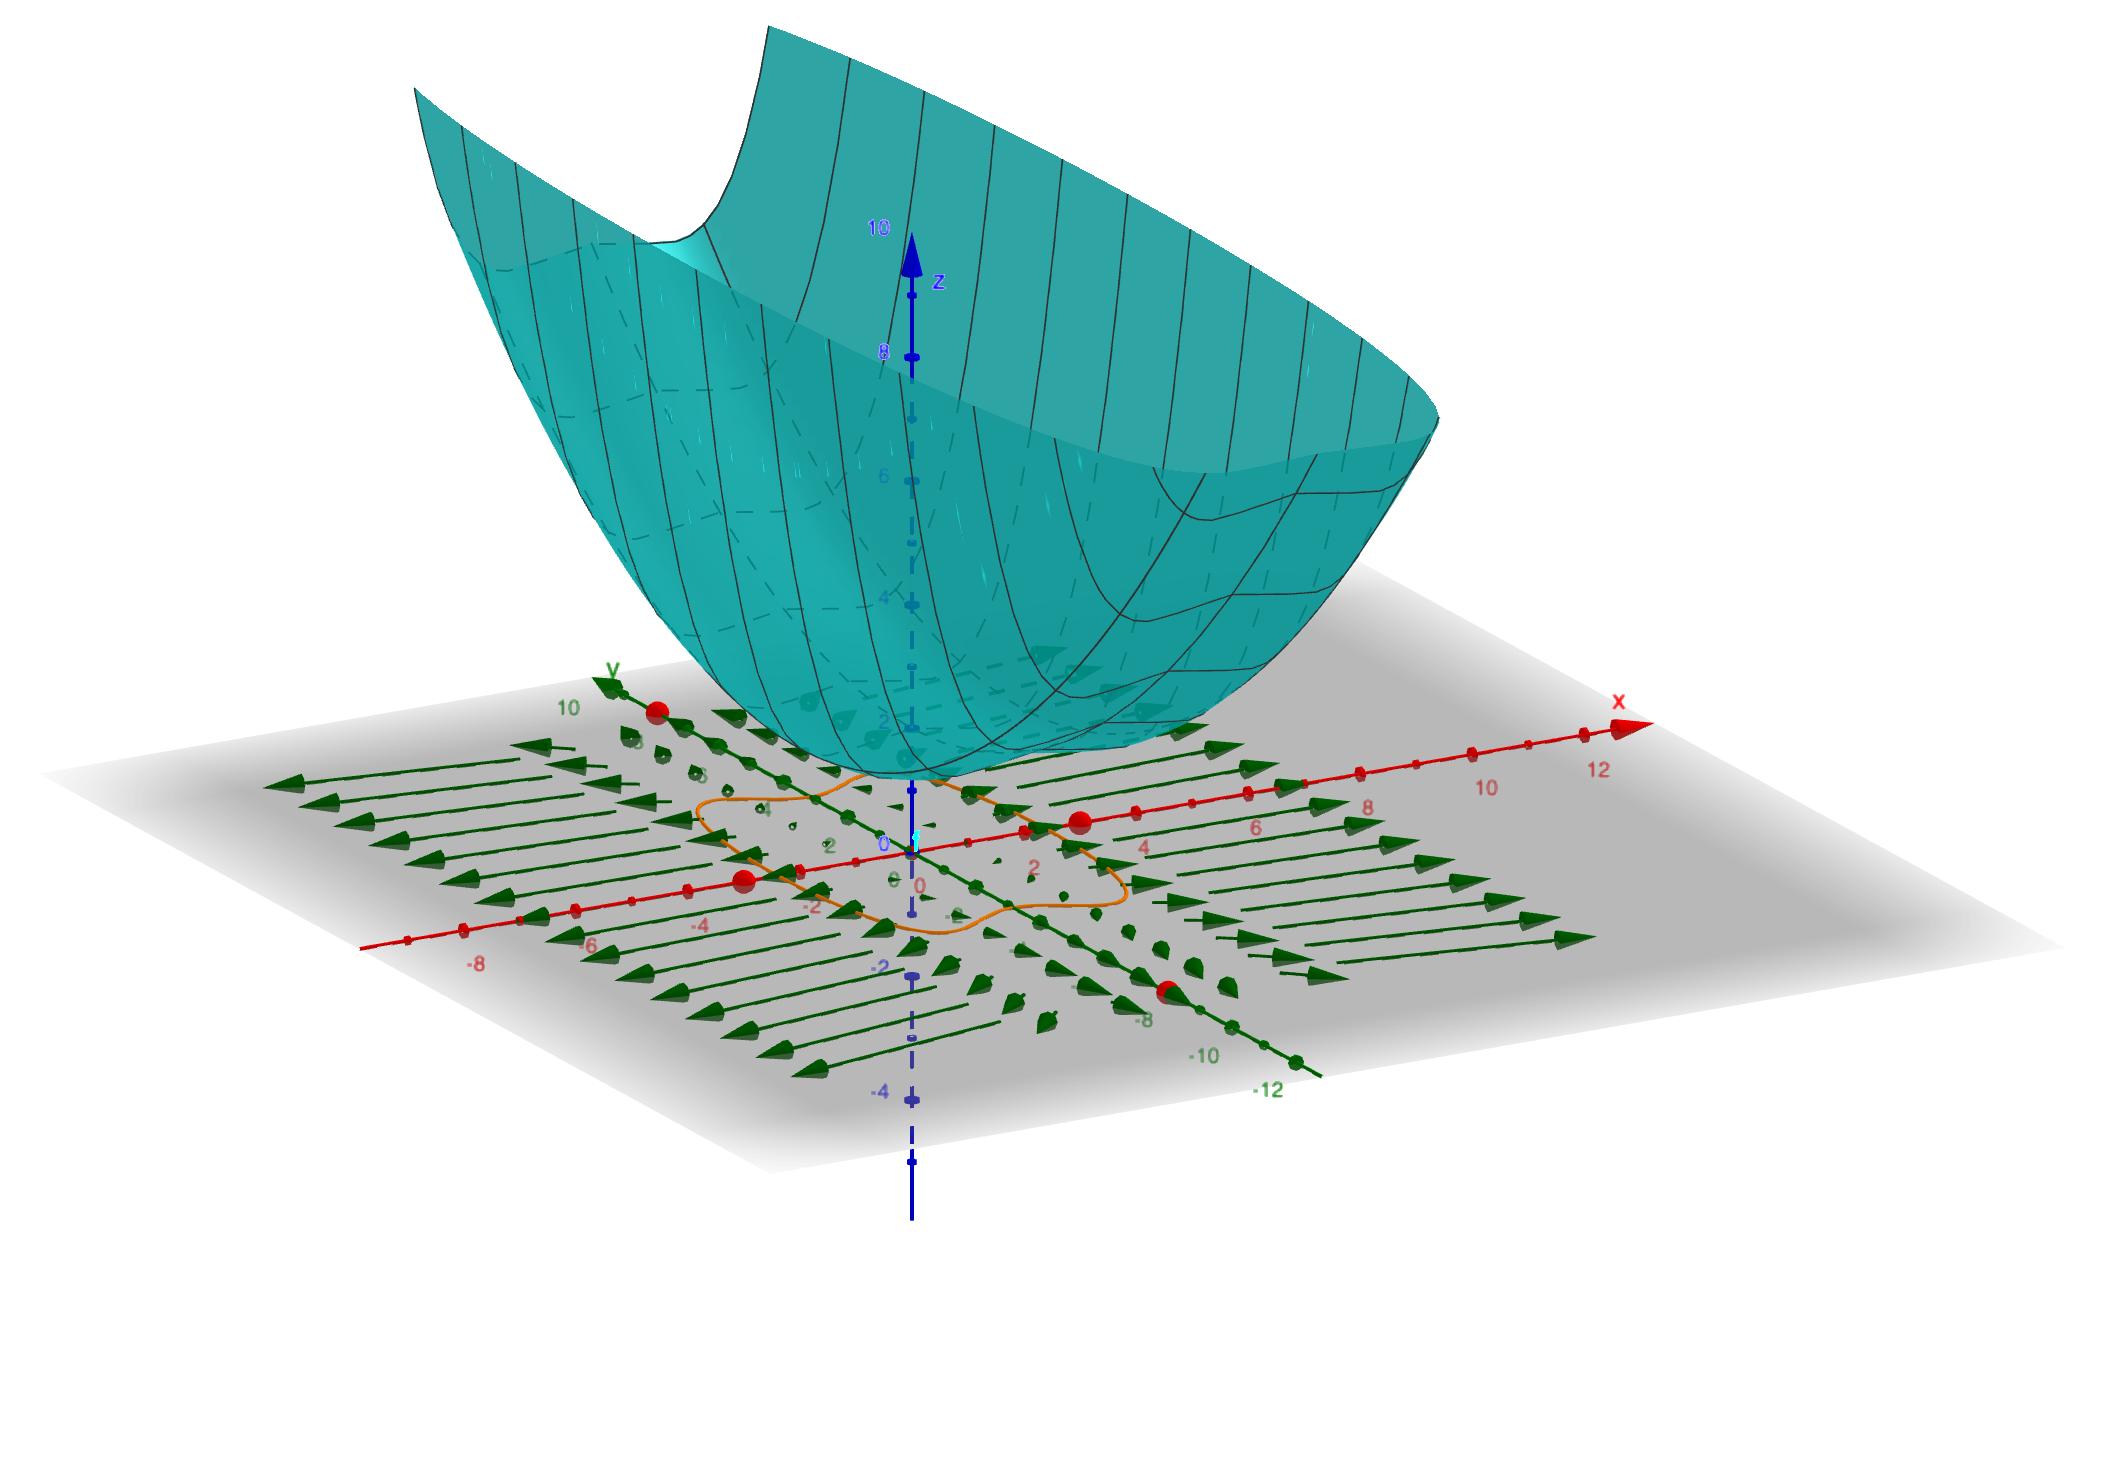
\includegraphics[width = \textwidth]{media/GradientenFeld.png}
%   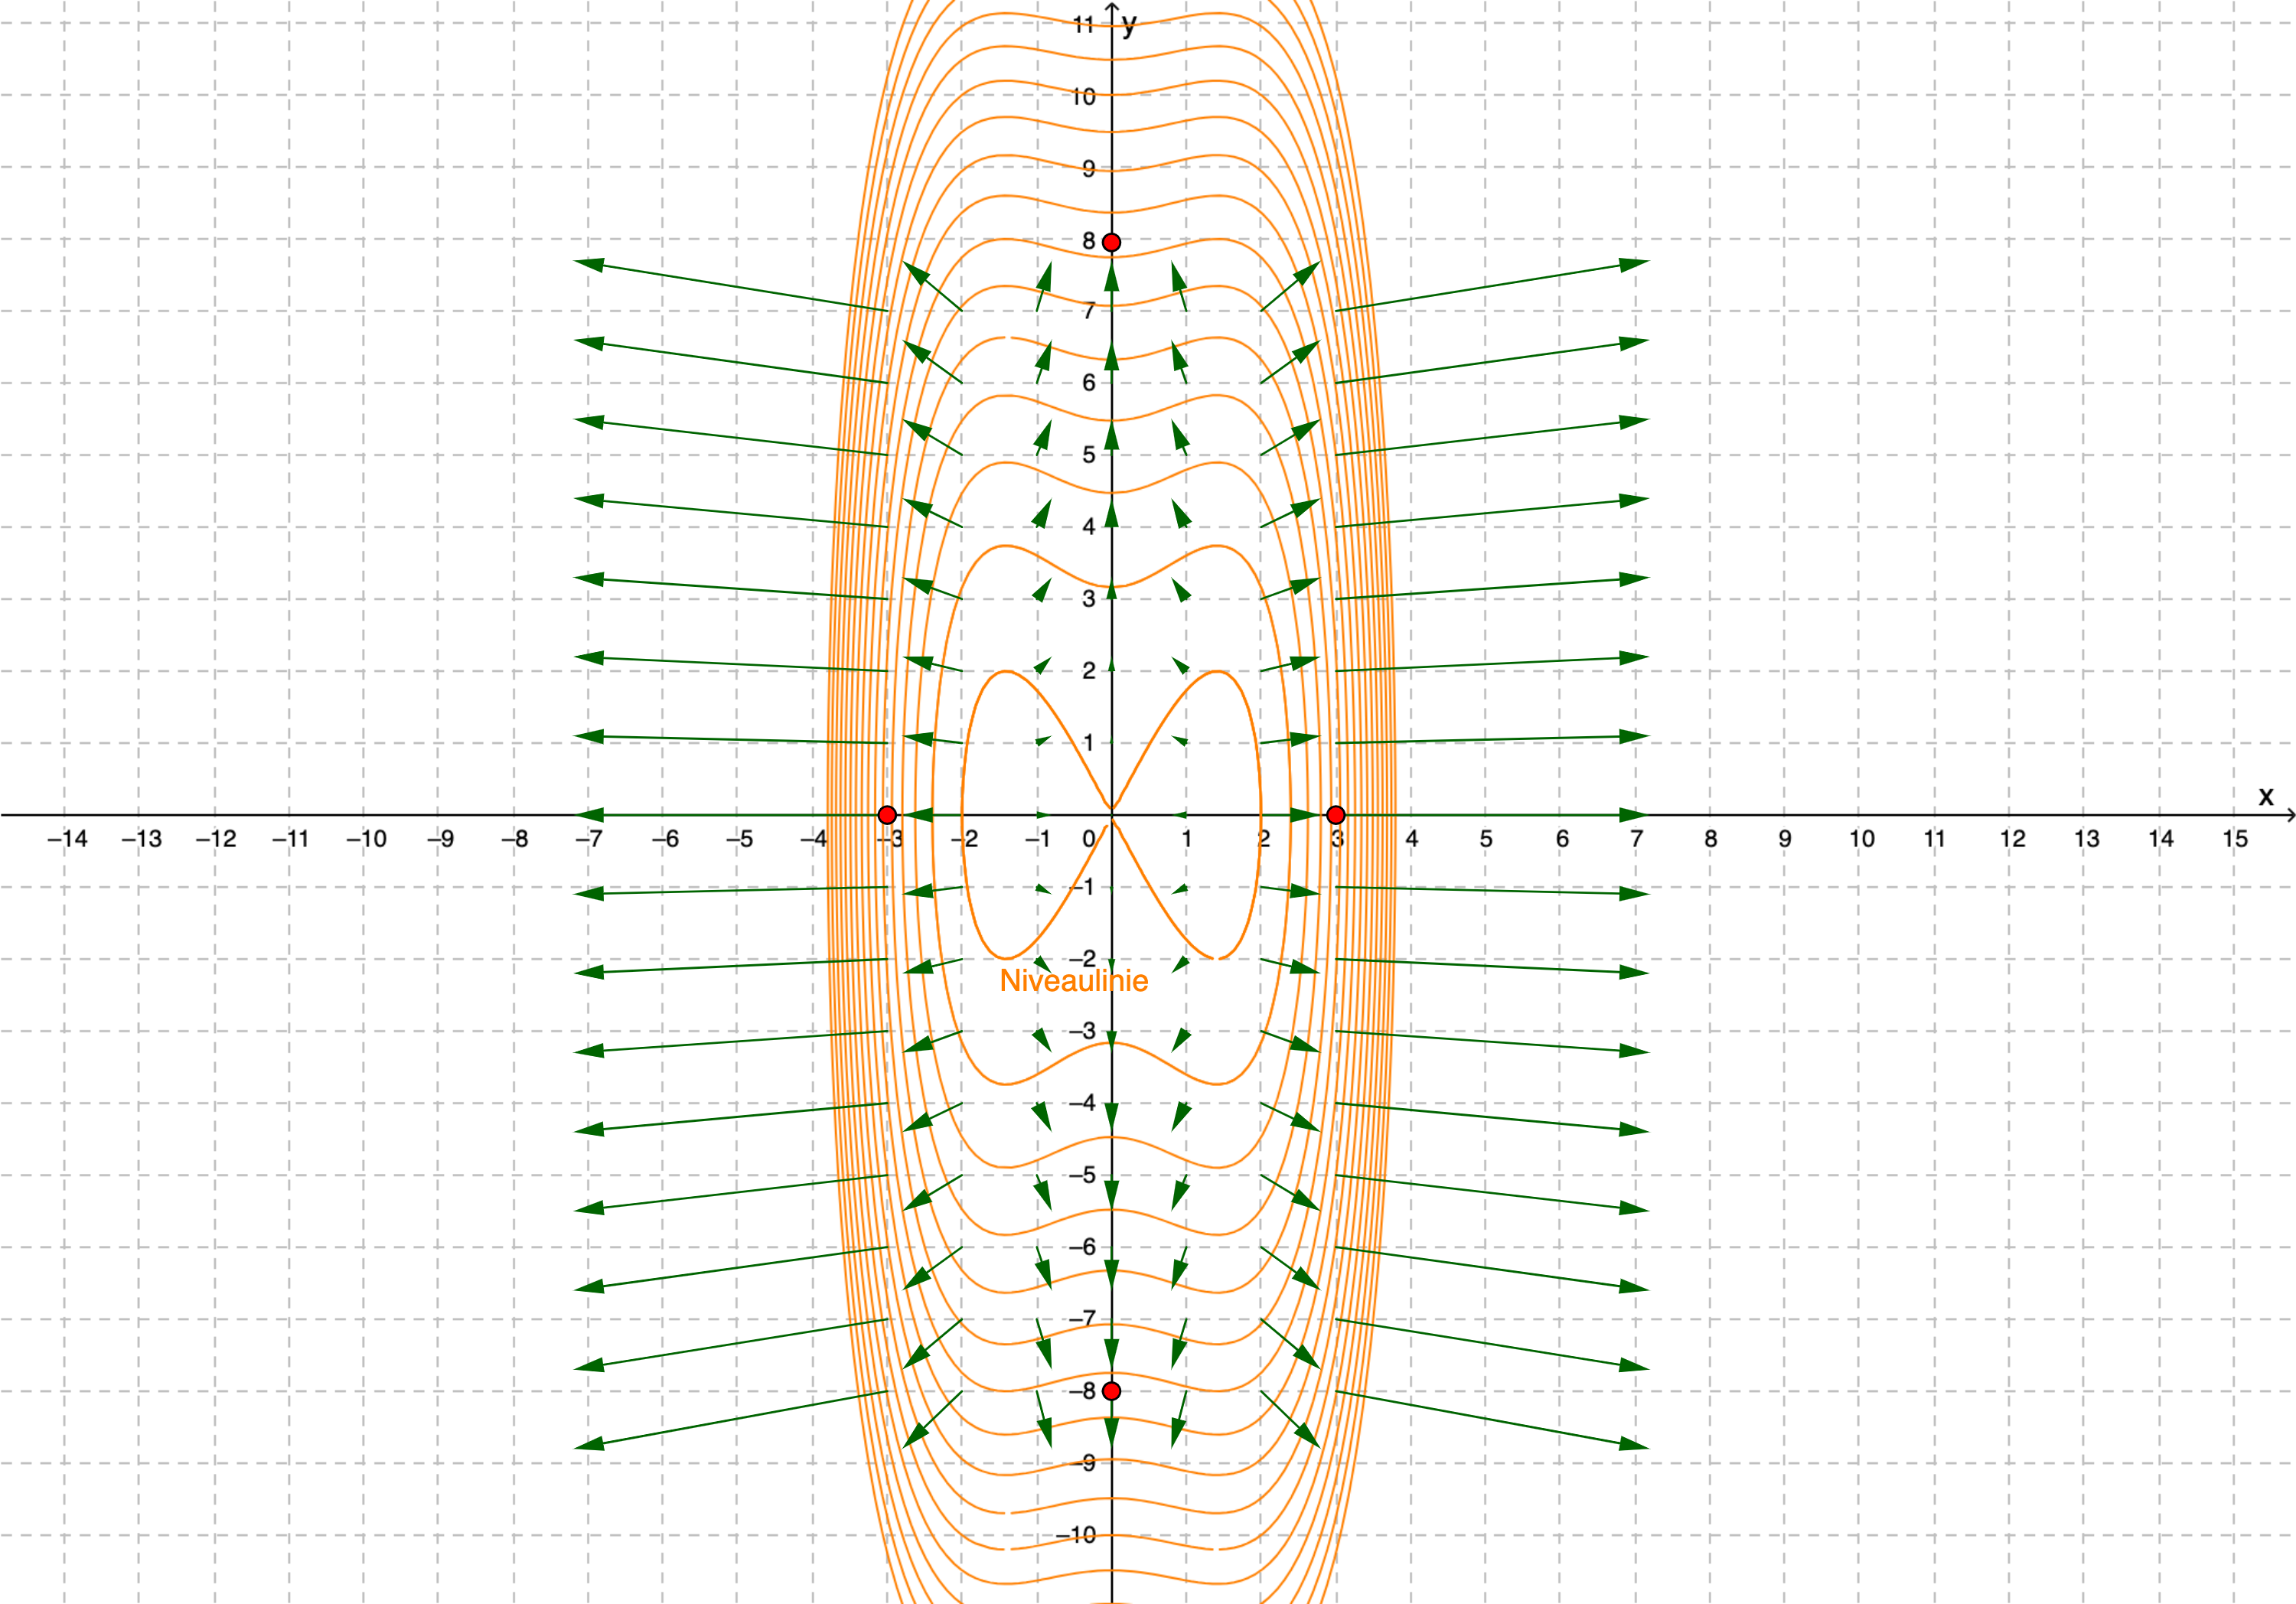
\includegraphics[width = \textwidth]{media/GradientNiveaulinie.png}

% \end{center}
\clearpage
\begin{ueb}
	{}{}

	\begin{enumerate}
		\item Gegeben ist die Funktion
		      \[
			      f(x, y) = 2x^2 y - 4xy + 3y^2.
		      \]
		      \begin{enumerate}
			      \item Bestimmen Sie den Gradienten \( \vec{\nabla} f(x, y) \).
			      \item Geben Sie die Richtungsableitung \(\frac{\partial f}{\partial \vec{v}}(2, -5) \) mit
			            \[
				            \vec{v} = \begin{pmatrix} -6 \\ 8 \end{pmatrix}
			            \]
			            an.
		      \end{enumerate}

		\item Die Gestalt einer Computerlandschaft ist gegeben durch die Gleichung
		      \[
			      z = 1 - 3x^2 - y^2 + 5 \cdot \sin(xy)
		      \]

		      Ein Ball befindet sich im Punkt
		      \[
			      P = (1 \mid 0 \mid f(1, 0))
		      \]
		      auf der Landschaft. In welche Richtung beginnt der Ball zu rollen, wenn die «Erdanziehung» in negativer \( z \)-Richtung wirkt?

		      \textit{Geben Sie den Tangentialvektor an die Bahn des Balls an.}

		      % \textbf{Tipp:} Die \( x \)- und \( y \)-Komponenten des gesuchten Vektors haben etwas mit dem Gradienten zu tun…  
		      % Für die \( z \)-Komponente müssen Sie Ihre «ersten Überlegungen» nochmals nachvollziehen…

		\item Gegeben ist die Funktion
		      \[
			      g(x, y) = e^{x^2 - 2y^2}, \quad P = (2 \mid 1)
		      \]
		      \begin{enumerate}
			      \item Bestimmen Sie den Gradienten der Funktion \( g \) im Punkt \( P \).
			      \item Zeigen Sie, dass sich der Punkt \( P \) auf der Höhenlinie zum Wert \( e^2 \) befindet, und geben Sie die Richtung des Tangentialvektors der Höhenlinie an.
		      \end{enumerate}
	\end{enumerate}

\end{ueb}
\clearpage
\emph{Lösungen}

\begin{enumerate}
	\item Funktion \( f(x, y) = 2x^2 y - 4xy + 3y^2 \)
	      \begin{enumerate}
		      \item Gradient:
		            \[
			            \vec{\nabla} f(x, y) =
			            \begin{pmatrix}
				            4x y - 4y \\
				            2x^2 - 4x + 6y
			            \end{pmatrix}
			            \Rightarrow
			            \vec{\nabla} f(2, -5) =
			            \begin{pmatrix}
				            -20 \\
				            -30
			            \end{pmatrix}
		            \]
		      \item Richtungsableitung in Richtung \( \vec{v} = \begin{pmatrix} -6 \\ 8 \end{pmatrix} \):
		            \[
			            \frac{\partial f}{\partial \vec{v}}(2, -5) = -120
		            \]
	      \end{enumerate}

	\item Landschaft: \( z = 1 - 3x^2 - y^2 + 5 \cdot \sin(xy) \)
	      \begin{itemize}
		      \item Gradient im Punkt \( (1, 0) \):
		            \[
			            \vec{\nabla} f(1, 0) = \begin{pmatrix} -6 \\ 5 \end{pmatrix}
		            \]
		      \item Tangentialvektor der Bahn (Richtung des stärksten Gefälles + Richtungsableitung als $z$-Komponente):
		            \[
			            \vec{v}_{\text{Bahn}} = \begin{pmatrix} 6 \\ -5 \\ 61 \end{pmatrix}
		            \]
	      \end{itemize}

	\item Funktion \( g(x, y) = e^{x^2 - 2y^2} \), Punkt \( P = (2, 1) \)
	      \begin{enumerate}
		      \item Gradient:
		            \[
			            \vec{\nabla} g(2, 1) = 4e^2
			            \begin{pmatrix}
				            1 \\
				            -1
			            \end{pmatrix}
		            \]
		      \item Höhenlinie bei \( g(2, 1) = e^2 \)

		            Tangentialvektor (orthogonal zum Gradienten):
		            \[
			            \vec{v} =
			            \begin{pmatrix}
				            1 \\
				            1
			            \end{pmatrix}
		            \]
	      \end{enumerate}
\end{enumerate}





















\clearpage
\subsection{Gradientenverfahren in machine Learning}
Viele Fragestellungen lassen sich heutzutage mit Computern lösen. Dabei werden die Computer so programmiert, dass sie eine Reihe von Anweisungen durchführen – einen Algorithmus – und so die gewünschte Lösung liefern.

Es gibt aber Fragestellungen, bei denen diese klassischen Vorgehensweise versagt. Das ist zum Beispiel dann der Fall, wenn man bestimmte Informationen richtig interpretieren soll. Ein typischen Beispiel dafür ist die Erkennung von Handschriften.

\begin{center}
	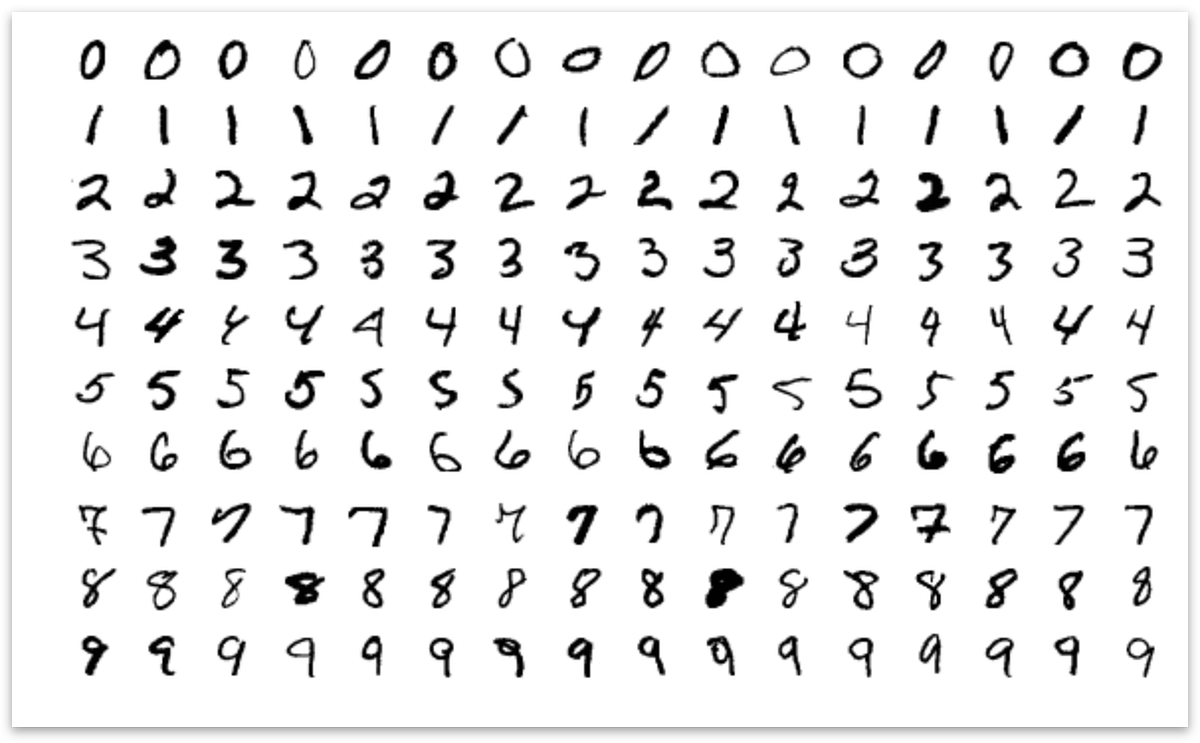
\includegraphics[width = \textwidth]{media/mnistDigit.png}
\end{center}

Während wir problemlos die Ziffern oben erkennen können, ist das für ein Computer keinesfalls einfach, weil die gleiche Ziffer ganz unterschiedlich dargestellt werden kann.
Für diese Fälle hat man in den vergangenen Jahren mit neuronalen Netzen grosse Erfolge erzielt. Dabei wird das Programm zuerst «trainiert», damit der Computer die richtigen Muster «erlernt». Im Grunde geht das wie folgt:

\begin{center}
	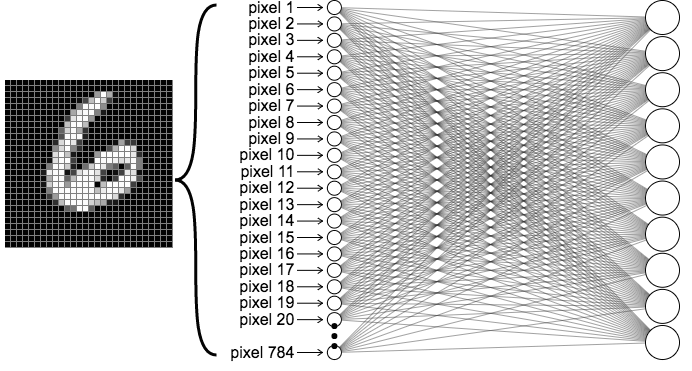
\includegraphics[width = \textwidth]{media/MnistArchitecture.png}
\end{center}


Das Programm erhält als Eingabe ein Bild. Im Beispiel handelt es sich um ein Schwarzweiss-Bild mit \( 28 \times 28 = 784 \) Pixeln.

Dieses Input-Bild kann als Vektor \( \vec{v} \) mit 784 Komponenten interpretiert werden. In der \( 30 \)-sten Komponente steht zum Beispiel, wie dunkel der entsprechende Pixel (2. Pixel in der 2. Zeile) ist – auf einer Skala von 0 bis 1.

\medskip

Dieser Vektor wird mit einer \( 10 \times 784 \)-Matrix \( M \) multipliziert\footnote{Das ist die Grundidee. In Wahrheit ist es etwas komplizierter.}. Damit erhält man einen neuen Vektor
\[
	\vec{w} = M \cdot \vec{v}
\]
mit 10 Einträgen. In diesem Vektor \( \vec{w} \) steht, wie wahrscheinlich das Bild eine bestimmte Ziffer darstellt:

\begin{itemize}
	\item Der 1. Eintrag steht für die Wahrscheinlichkeit, dass die Ziffer eine Eins ist,
	\item der 4. Eintrag z.\,B. für eine Vier,
	\item der 10. Eintrag für eine Null.
\end{itemize}

\medskip

\textbf{Zentrale Frage:} Wie lauten die 7840 Einträge der Matrix \( M \)?

Die Kernidee des \emph{maschinellen Lernens} ist, dass der Computer diese Einträge \textbf{selbstständig lernen} kann!

\medskip

Zunächst beginnt man mit einer zufälligen Startmatrix \( M \) und verbessert diese schrittweise. Dazu verwendet man ein bekanntes Eingabebild – zum Beispiel das einer 6 – und berechnet den Output-Vektor:
\[
	\vec{w} = M \cdot \vec{v}
\]


Die Komponenten des Vektors \( \vec{w} \) sind zu Beginn meist zufällig verteilt, etwa so:
\[
	\vec{w} =
	\begin{pmatrix}
		0.2 \\
		0.1 \\
		0.8 \\
		0.6 \\
		0.2 \\
		0.4 \\
		0.6 \\
		0.9 \\
		0.3 \\
		0.1
	\end{pmatrix}
\]

Da das Bild eine \textbf{Sechs} darstellt, sollte idealerweise jeder Eintrag des Outputvektors \( \vec{w} \) gleich null sein – mit Ausnahme des sechsten Eintrags, der den Wert 1 haben sollte.

\medskip

So entsteht ein \textbf{Fehlervektor}:
\[
	\vec{f} = \vec{w} - \vec{z} =
	\begin{pmatrix}
		-0.2 \\
		-0.1 \\
		-0.8 \\
		-0.6 \\
		-0.2 \\
		0.6  \\
		-0.6 \\
		-0.9 \\
		-0.3 \\
		-0.1
	\end{pmatrix}
\]
wobei \( \vec{z} \) der Zielvektor ist mit Eins an sechster Stelle und sonst Nullen.

\medskip

Das \textbf{Quadrat der Länge} des Fehlervektors ergibt den Fehlerwert:
\[
	F = |\vec{f}|^2 = (-0.2)^2 + (-0.1)^2 + \cdots + (-0.1)^2
\]

Offensichtlich hängt die Grösse von \( F \) von den Einträgen $m_{1,1}, m_{1,2}, \dotsc, m_{10,784}$ der Matrix \( M \) ab.
Man kann \( F \) daher als Funktion
\[
	F = F\left(m_{1,1}, m_{1,2}, \dotsc, m_{10,784}\right)
\]
auffassen – also eine Funktion in 7840 Variablen!

\medskip

Im Lernprozess wird die Matrix \( M \) nun so verändert, dass der Fehler \( F \) kleiner wird.
Hier kommt der \textbf{Gradient} ins Spiel:
Die grösste Abnahme von \( F \) geschieht in Richtung \( -\vec{\nabla}F \).

\medskip

Man erhält eine neue Matrix \( M_{\text{neu}} \), deren Einträge aus der Summe der entsprechenden Einträge von \( M \) und \( -\vec{\nabla}F \) gebildet werden:
\[
	M_{\text{neu}} = M - k \cdot \vec{\nabla}F
\]
(wobei \( k \) die sogenannte `Lernrate' ist).

\medskip

Dieser Vorgang wird wiederholt – jeweils mit unterschiedlichen Trainingsbildern –, bis das Programm die gewünschten Ergebnisse liefert.














\begin{LA}
	{Aufgabe: Anwendung des Gradienten auf neuronale Netzwerke}{}


	Ein Computerprogramm soll mit einem (vereinfachten) neuronalen Netzwerk lernen, Zahlen zu addieren und zu subtrahieren.

	Das Programm erhält als Input zwei Zahlen \( v_1 \) und \( v_2 \), die wir als Vektor
	\[
		\vec{v} = \begin{pmatrix} v_1 \\ v_2 \end{pmatrix}
	\]
	auffassen, und berechnet den Output
	\[
		\vec{w} = \begin{pmatrix} w_1 \\ w_2 \end{pmatrix} = M \cdot \vec{v},
	\]
	wobei \( M \) eine \( 2 \times 2 \)-Matrix ist, die zu Beginn zufällig gewählt ist und mit dem Gradient-Descent-Verfahren laufend verbessert werden soll, sodass der gewünschte Zieloutput
	\[
		\vec{z} = \begin{pmatrix} v_1 + v_2 \\ v_1 - v_2 \end{pmatrix}
	\]
	damit berechnet wird.

	\medskip

	Zu Beginn soll die Matrix die Einträge
	\[
		M = \begin{pmatrix} 1 & 2 \\ 3 & 4 \end{pmatrix}
	\]
	aufweisen. Das neuronale Netzwerk wird mit der Eingabe
	\[
		\vec{v} = \begin{pmatrix} 2 \\ 1 \end{pmatrix}
	\]
	trainiert.

	\begin{itemize}
		\item Berechnen Sie den Output \( \vec{w} \) des neuronalen Netzwerks, den Fehlervektor \( \vec{f} = \vec{w} - \vec{z} \) und dessen quadrierten Betrag \( F = |\vec{f}|^2 \).\\
		      \textit{(Kontrolle: \( \vec{w} = \begin{pmatrix} 4 \\ 10 \end{pmatrix} \), \( \vec{f} = \begin{pmatrix} 1 \\ 9 \end{pmatrix} \), \( F = 82 \))}
	\end{itemize}

	Als nächstes soll die Matrix so verändert werden, dass der Fehler kleiner wird. Dazu betrachten wir den Fehler \( F \) als Funktion der Einträge der Matrix
	\[
		M = \begin{pmatrix} a & b \\ c & d \end{pmatrix}.
	\]

	\begin{itemize}
		\item Berechnen Sie nochmals den Fehler \( F = |\vec{f}|^2 \) mit dem Input \( \vec{v} = \begin{pmatrix} 2 \\ 1 \end{pmatrix} \), wobei \( M \) nun allgemein \( \begin{pmatrix} a & b \\ c & d \end{pmatrix} \) ist.\\
		      \textit{(Kontrolle: \( F(a,b,c,d) = (2a + b - 3)^2 + (2c + d - 1)^2 \))}
	\end{itemize}

	Den Fehler fassen wir ab jetzt als Funktion mit vier Argumenten \( a, b, c, d \) auf.
	Den Graphen von \( F \) könnte man als 4-dimensionale Hyperfläche in einem 5-dimensionalen Raum realisieren.
	Hier versagt die Vorstellungskraft – wir können aber die Ideen der Funktionen in zwei Variablen nutzen!

	\medskip

	Wir ändern die Inputs \( a, b, c, d \) (also die Einträge der Matrix \( M \)) so, dass der Fehler kleiner wird.
	Wie stark soll jeder Eintrag verändert werden? Der Gradient liefert die Antwort:

	\begin{itemize}
		\item Berechnen Sie den Gradienten \( \vec{\nabla}F \) der Funktion \( F(a,b,c,d) \) an der Stelle \( (a_0, b_0, c_0, d_0) = (1, 2, 3, 4) \).\\
		      \textit{(Kontrolle: \( \vec{\nabla}F(1,2,3,4) = \begin{pmatrix} 4 \\ 2 \\ 36 \\ 18 \end{pmatrix} \))}
	\end{itemize}

	Der Gradient zeigt in Richtung des stärksten Anstiegs der Fehlerfunktion \( F \).
	Um die Einträge der Matrix \( M \) so zu verändern, dass der Fehler kleiner wird, müssen diese also in Richtung \( -\vec{\nabla}F \) verändert werden.

	\medskip

	Allerdings sind die Einträge des Gradienten sehr gross.
	Wenn wir die Einträge der Matrix \( M \) einen Schritt in Richtung Gradient verändern, würden wir an den Werten für den minimalen Fehler «vorbeischiessen».
	Aus diesem Grund verändern wir die Einträge nur um \( \frac{1}{20} \cdot \vec{\nabla}F \).
	(Der Faktor \( k = \frac{1}{20} \) heisst \emph{Lernrate}.)

	\begin{itemize}
		\item Fassen Sie die Matrix \( M = \begin{pmatrix} 1 & 2 \\ 3 & 4 \end{pmatrix} \) als Vektor \( \vec{m} = \begin{pmatrix} 1 \\ 2 \\ 3 \\ 4 \end{pmatrix} \) auf. Berechnen Sie:
		      \[
			      \vec{m}_{\text{neu}} = \vec{m} - \frac{1}{20} \cdot \vec{\nabla}F(1,2,3,4)
		      \]
		      Wandeln Sie das Resultat wieder in eine Matrix \( M_{\text{neu}} \) um und berechnen Sie den neuen Fehler \( F_{\text{neu}} \).\\
		      \textit{(Kontrolle: \( F_{\text{neu}} = 20.5 \))}
	\end{itemize}

	Der Wert der Fehlerfunktion \( F \) ist deutlich kleiner geworden.
	Wird dieses Training mehrmals mit unterschiedlichen Eingaben durchgeführt, so nähert sich die Matrix \( M \) schrittweise der Matrix
	\[
		M_\infty = \begin{pmatrix} 1 & 1 \\ 1 & -1 \end{pmatrix}.
	\]

	Auf diese Art lernt das Programm, welche Werte die Matrix haben muss, um zwei Zahlen zu addieren und zu subtrahieren.

	\bigskip

	\textbf{Zusatzfrage:}
	Zeigen Sie: Hätten wir als Lernrate \( \frac{1}{10} \) gewählt, hätten wir \( F_{\text{neu}} = 0 \) erhalten.
	Die Matrix \( M_{\text{neu}} \) berechnet aber nur \emph{für diesen Vektor} den richtigen Output.
	In Wirklichkeit wird das neuronale Netzwerk mit ganz vielen unterschiedlichen In- und Ziel-Outputs trainiert.

\end{LA}

























\clearpage
\subsection{Vermischte Aufgaben}
\begin{ueb}
	{}{}
	\begin{enumerate}
		\item Bestimmen Sie den Gradienten der folgenden Funktionen:
		      \begin{enumerate}
			      \item \( f(x, y) = x^2 + y^2 \)
			      \item \( g(x, y) = e^{x - y} \)
			      \item \( h(x, y) = \sin(x) \cdot \cos(y) \)
		      \end{enumerate}

		\item
		      Betrachten wir einen Massenpunkt, der im Ursprung unseres Koordinatensystems so gelagert ist, dass seine Auslenkung in Richtung der Koordinatenachsen, etwa durch zwei Federn realisiert, eine Rückstellkraft proportional zur Auslenkung erfährt, die in $y$-Richtung doppelt so gross sei, wie in $x$-Richtung.
		      \begin{center}
			      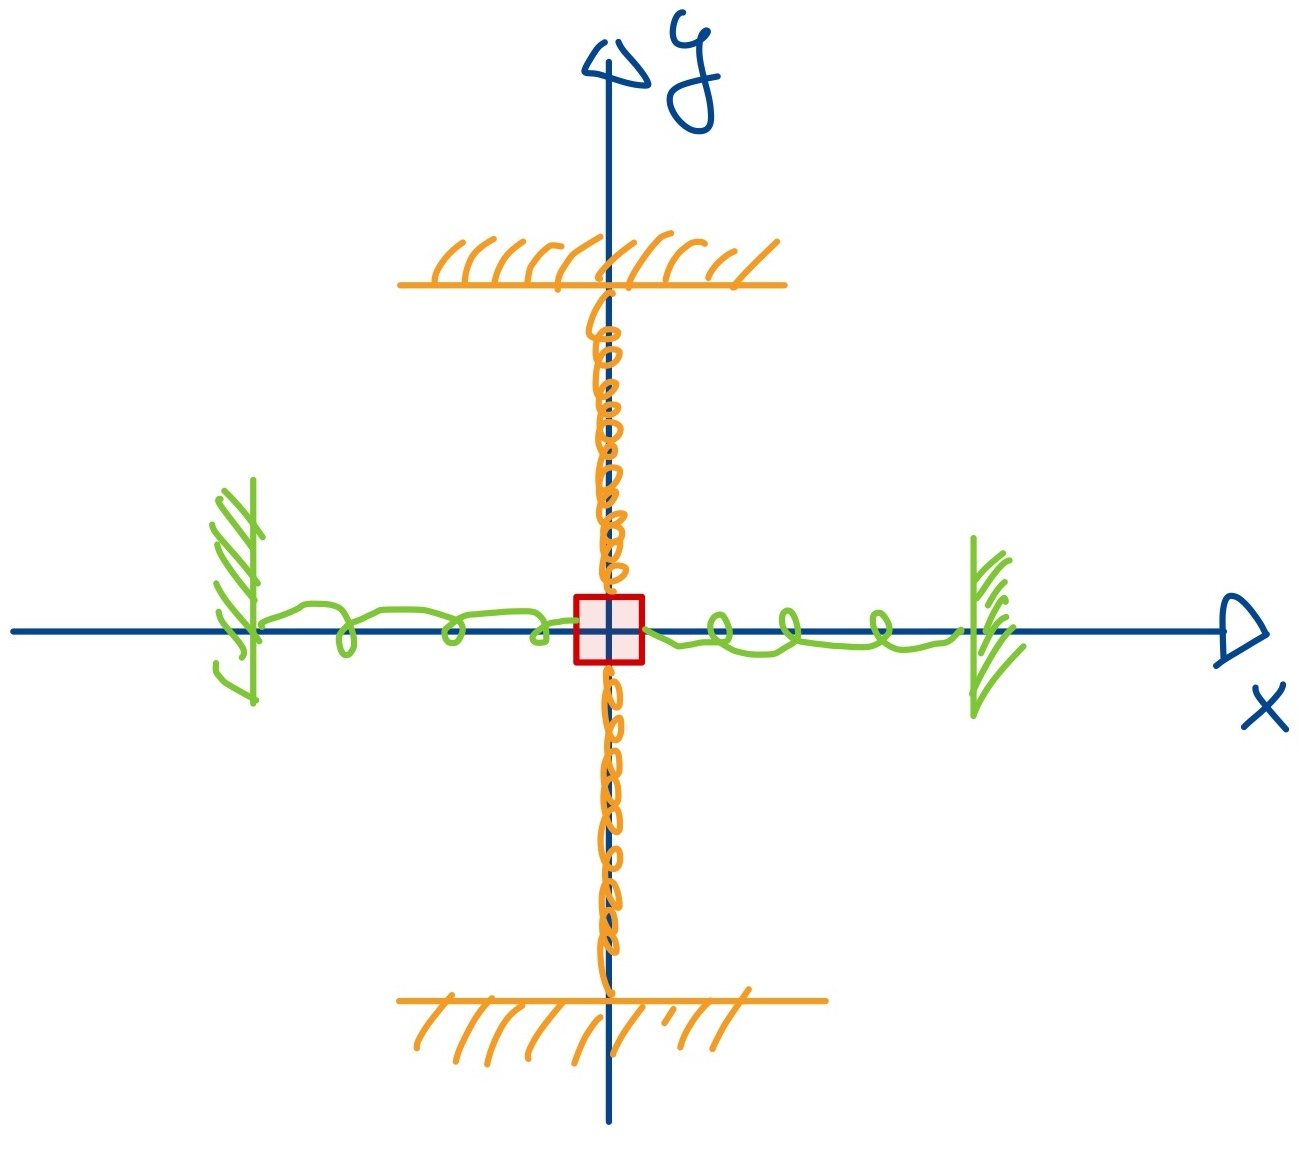
\includegraphics[width = 0.4\textwidth]{media/harm-osz-1.jpg}
		      \end{center}

		      Die potenzielle Energie $V(x,y)$ bei einer Auslenkung $(x,y)$ aus der Ruhelage ist dann (Bei Federkonstanten 1 bzw. 2):
		      \[
			      V(x, y) = \frac{1}{2}x^2 + y^2
		      \]
		      \begin{enumerate}
			      \item Geben Sie die Gleichung der Niveaulinie \( N_1 \) zum Wert \( V = 1 \) an. Es handelt sich um eine Ellipse!
			            Geben Sie die Halbachsen an und fertigen Sie eine Skizze.

			            \emph{Hinweis}: Ellipsen haben eine Gleichung der Form
			            $$\frac{x^2}{a^2} + \frac{y^2}{b^2} = 1$$
			            mit den Halbachsen \( a \) und \( b \).
			      \item Zeigen Sie, dass der Punkt \( P = \left( 1, \frac{\sqrt{2}}{2} \right) \) auf \( N_1 \) liegt.
			      \item Berechnen Sie den Gradienten an der Stelle \( P \). Welche Bedeutung hat das Resultat im Kontext des harmonischen Oszillators?
			      \item Geben Sie die Gleichung der Tangente an \( N_1 \) im Punkt \( P \) an.
		      \end{enumerate}

		\item Die Temperatur einer in der \( xy \)-Ebene liegenden Platte sei gegeben durch:
		      \[
			      T(x, y) = \frac{1}{1 + x^2 + y^2}, \qquad x,y \text{ Position in Meter, } \quad T \text{ in Grad Celsius}
		      \]
		      \begin{enumerate}
			      \item Berechnen Sie den Gradienten in jedem Punkt.
			      \item In welche Richtung ist der Temperaturanstieg am grössten?
			      \item Schliessen Sie vom Gradienten auf die Gestalt der Niveaulinien.
			      \item Ein Massenpunkt bewegt sich entlang einer Geraden in Richtung $\begin{pmatrix}
					            1 \\ 3
				            \end{pmatrix}$. Berechnen Sie den lokalen Temperaturanstieg in Grad Celsius/Meter beim Passieren des Punktes \( (2, 3) \) in Richtung der Geraden.
			            % \(
			            % \begin{pmatrix}
			            % 1 \\ 3
			            % \end{pmatrix}
			            % \)
			            %in \( ^\circ\mathrm{C}/\mathrm{LE} \).
		      \end{enumerate}

		\item Durch ein Gelände mit der Höhenfunktion
		      \[
			      h(x, y) = \frac{1000 + x + y + \sqrt{xy + 76}}{10}
		      \]
		      wird längs der Geraden
		      \[
			      \vec{r}(t) = \begin{pmatrix} 1 \\ 2 \end{pmatrix} + t \cdot \begin{pmatrix} 3 \\ 4 \end{pmatrix}
		      \]
		      eine Strasse gebaut. Bestimmen Sie die Steigung der Strasse an der Stelle \( (x, y) = (4, 6) \).

		\item Gegeben sei die Funktion
		      \[
			      f(x, y) = \sin(x) + \sin(y) + \sin(x + y)
		      \]
		      \begin{enumerate}
			      \item Wie gross ist die Steigung der Tangente an die Schnittkurve des Graphen von \( f \) mit einer zur \( xz \)-Ebene parallelen Ebene im Punkt \( P = \left( \frac{\pi}{2}, \frac{\pi}{4}, ? \right) \)?
			      \item Geben Sie eine Gleichung der Tangentialebene an den Graphen im Ursprung an.
		      \end{enumerate}
	\end{enumerate}
\end{ueb}



\clearpage
\emph{Lösungen}


\begin{enumerate}
	\item \textbf{Gradienten}
	      \begin{enumerate}
		      \item \( \vec{\nabla} f(x, y) = 2 \begin{pmatrix} x \\ y \end{pmatrix} \)
		      \item \( \vec{\nabla} g(x, y) = e^{x - y} \begin{pmatrix} 1 \\ -1 \end{pmatrix} \)
		      \item \( \vec{\nabla} h(x, y) = \begin{pmatrix}
			            \cos(x) \cos(y) \\
			            -\sin(x) \sin(y)
		            \end{pmatrix} \)
	      \end{enumerate}

	\item \textbf{Harmonischer Oszillator}
	      \begin{enumerate}
		      \item Niveaulinie \( N_1 \): \( \frac{x^2}{2} + y^2 = 1 \)
		            Ellipse mit Halbachsen \( \sqrt{2} \) und \( 1 \).
		      \item \( V\left(1, \frac{\sqrt{2}}{2}\right) = \frac{1}{2} + \frac{1}{2} = 1 \)
		      \item \( \vec{\nabla} V\left(1, \frac{\sqrt{2}}{2}\right) = \begin{pmatrix} 1 \\ \sqrt{2} \end{pmatrix} \) Bewegt sich der Massepunkt ausgehend von \( P \) in Richtung des Gradienten, so steigt die Energie am schnellsten an.
		      \item Tangente an \( N_1 \) im Punkt \( P \):
		            \[
			            \vec{r}(t) = \begin{pmatrix} 1 \\ \frac{\sqrt{2}}{2} \end{pmatrix} + t \cdot \begin{pmatrix} -\sqrt{2} \\ 1 \end{pmatrix}
			            \quad \text{oder} \quad y = -\frac{\sqrt{2}}{2} x + \sqrt{2}
		            \]
	      \end{enumerate}

	\item \textbf{Temperaturfeld}
	      \begin{enumerate}
		      \item Gradient:
		            \[
			            \vec{\nabla} T(x, y) = -\frac{2}{(1 + x^2 + y^2)^2} \begin{pmatrix} x \\ y \end{pmatrix}
		            \]
		      \item Der Temperaturanstieg ist in Richtung des Ursprungs am grössten.
		      \item Die Normale zur Niveaulinie zeigt stets zum Ursprung. Die Niveaulinien sind also Kreise mit Zentrum im Ursprung.
		      \item Richtungsableitung bei \( (2, 3) \) in die normierte Richtung \( \frac{1}{\sqrt{10}} \begin{pmatrix} 1 \\ 3 \end{pmatrix} \):
		            \[
			            \frac{\partial T}{\partial \vec{v}}(2, 3) = -\frac{11}{98\sqrt{10}}
		            \]
	      \end{enumerate}

	\item \textbf{Gelände und Strasse}
	      \begin{enumerate}
		      \item Steigung entlang \( \vec{v} = \begin{pmatrix} 3 \\ 4 \end{pmatrix} \) bei \( (4, 6) \):
		            \[
			            \frac{1}{5} \frac{\partial h}{\partial \vec{v}}(4, 6) = \frac{87}{500}
		            \]
	      \end{enumerate}

	\item \textbf{Funktion mit Sinus-Termen}
	      \begin{enumerate}
		      \item \(\frac{\partial f}{\partial x} \left(\frac{\pi}{2}, \frac{\pi}{4}\right) = -\frac{\sqrt{2}}{2} \)
		      \item Tangentialebene im Ursprung:
		            \[
			            T: z = 2x + 2y
		            \]
	      \end{enumerate}
\end{enumerate}

\clearpage
\section{Kritische Punkte}
\label{sec:kritischePunkte}

Zur Erinnerung: Bei einer Funktion in einer Variablen kann man die Extremalpunkte leicht wie folgt finden:
\begin{enumerate}
	\item Man ermittelt die sogenannten kritischen Stellen. Das sind jene Stellen, in denen der Graph eine horizontale Tangente aufweist, und entsprechen somit den Nullstellen der Ableitung.
	\item Die Art des Punktes kann mit der zweiten Ableitung ermittelt werden: Ist die zweite Ableitung an einer kritischen Stelle positiv, so liegt ein lokales Minimum vor. Falls die zweite Ableitung negativ ist, befindet sich an der entsprechenden Stelle ein lokales Maximum.
\end{enumerate}
Auf den folgenden Seiten werden wir ähnliche Kriterien für Funktionen in zwei Variablen erarbeiten.

\subsection{Kritische Punkte}

Die kritischen Punkte sind im Falle von Funktionen in zwei Variablen jene Punkte, in denen die Tangentialebene an den Graphen parallel zur $xy$-Ebene verläuft.
\begin{center}
	\begin{tikzpicture}
		\begin{axis}[
				view={120}{30},
				axis lines=center,
				xlabel={$x$},
				ylabel={$y$},
				zlabel={$z$},
				domain=-1:1,
				y domain=-1:1,
				samples=30,
				colormap/cool,
			]
			% Surface plot (flipped to represent a maximum)
			\addplot3[surf, opacity=0.7] {-x^2 - y^2 + 4};

			% Tangent plane at the maximum
			\addplot3[surf, opacity=0.25, colormap/blackwhite]
			coordinates {
					(-1, -1, 4) (-1, 1, 4) (1, -1, 4) (1, 1, 4)
				};

			% Critical point (maximum)
			\addplot3[mark=*, color=red] coordinates {(0, 0, 4)};
		\end{axis}
	\end{tikzpicture}
\end{center}

Unter den kritischen Punkten unterscheidet man grob drei Arten: lokale Maxima, lokale Minima und Sattelpunkte.

\begin{center}
	\begin{tikzpicture}
		\begin{axis}[
				view={120}{30},
				axis lines=center,
				xlabel={$x$},
				ylabel={$y$},
				zlabel={$z$},
				domain=-1:1,
				y domain=-1:1,
				samples=30,
				colormap/cool,
				width=0.3\textwidth,
			]
			% Maximum
			\addplot3[surf, opacity=0.7] {-x^2 - y^2 + 4};
			\addplot3[mark=*, color=red] coordinates {(0, 0, 4)};
		\end{axis}
	\end{tikzpicture}
	\hfill
	\begin{tikzpicture}
		\begin{axis}[
				view={120}{30},
				axis lines=center,
				xlabel={$x$},
				ylabel={$y$},
				zlabel={$z$},
				domain=-1:1,
				y domain=-1:1,
				samples=30,
				colormap/cool,
				width=0.3\textwidth,
			]
			% Minimum
			\addplot3[surf, opacity=0.7] {x^2 + y^2 - 4};
			\addplot3[mark=*, color=blue] coordinates {(0, 0, -4)};
		\end{axis}
	\end{tikzpicture}
	\hfill
	\begin{tikzpicture}
		\begin{axis}[
				view={120}{30},
				axis lines=center,
				xlabel={$x$},
				ylabel={$y$},
				zlabel={$z$},
				domain=-1:1,
				y domain=-1:1,
				samples=30,
				colormap/cool,
				width=0.3\textwidth,
			]
			% Saddle point
			\addplot3[surf, opacity=0.7] {x^2 - y^2};
			\addplot3[mark=*, color=green] coordinates {(0, 0, 0)};
		\end{axis}
	\end{tikzpicture}
\end{center}

Da die Tangentialebene in diesen Punkten horizontal verläuft, hat sie eine Gleichung der Form
\[
	z = c
\]
Das heisst, dass in der Gleichung die Variablen \(x\) und \(y\) nicht vorkommen, bzw. dass deren Koeffizienten Null sind. Allgemein haben aber Tangentialebenen an den Graphen einer Funktion \(f\) an der Stelle \((x_0, y_0)\) die Gleichung
\[
	z = f(x_0, y_0) + \frac{\partial f}{\partial x}(x_0, y_0) \cdot (x - x_0) + \frac{\partial f}{\partial y}(x_0, y_0) \cdot (y - y_0)
\]
Die Koeffizienten von \(x\) und \(y\) sind im Allgemeinen also \(\frac{\partial f}{\partial x}(x_0, y_0)\) und \(\frac{\partial f}{\partial y}(x_0, y_0)\). Die Tangentialebene \(f\) an der Stelle \((x_0, y_0)\) verläuft also genau dann parallel zur \(xy\)-Ebene, wenn
\[
	\frac{\partial f}{\partial x}(x_0, y_0) = 0 \quad \text{und} \quad \frac{\partial f}{\partial y}(x_0, y_0) = 0
\]
ist.


\begin{definition}
	{Kritische Stellen}{}
	Die kritischen Stellen einer Funktion \(f(x, y)\) sind jene Stellen \((x_0, y_0)\), für welche gilt:
	\[
		\vec{\nabla} f(x_0, y_0) = \vec{0}
	\]
\end{definition}

\begin{bsp}
	{}{}
	$$f(x,y)=x^2+xy-y$$
	\vspace*{8cm}
\end{bsp}
\clearpage
\begin{bsp}
	{}{kritischePunkte2}
	$$f(x,y)=x^3+xy^2-x$$
	\vspace*{15cm}
\end{bsp}

\begin{ueb}
	{}{}
	\begin{enumerate}
		\item Bestimmen Sie die kritischen Stellen der folgenden Funktionen und zeichnen Sie deren Graphen mit Geogebra:
		      \begin{enumerate}
			      \item \(f(x,y) = -10x + 2xy + y^3\)
			      \item \(f(x,y) = x^2y - x^2 - y^2\)
			      \item \(f(x,y) = e^{x^2 + 4x + y^2}\)
		      \end{enumerate}
	\end{enumerate}
\end{ueb}

\clearpage
\emph{Lösungen}
\begin{enumerate}
	\item \(K = \left(-\frac{75}{2}, 5\right)\)
	\item \(K_1 = (0, 0), \, K_2 = \left(\sqrt{2}, 1\right), \, K_3 = \left(-\sqrt{2}, 1\right)\)
	\item \(K = (-2, 0)\)
\end{enumerate}

















\clearpage
\subsection{Hesse-Matrix}
\label{sec:hesseMatrix}
Im letzten Kapitel haben Sie eine Methode kennengelernt, wie man die kritischen Punkte einer Funktion finden kann. Allerdings bleibt noch die Frage, ob es sich dabei um lokale Minima, Maxima oder Sattelpunkte handelt. Wie bei Funktionen in einer Variablen werden wir dazu die zweite Ableitung betrachten. Davon gibt es aber mehrere!

Betrachten wir die Funktion \(f(x,y) = x^2 + 2xy^2 + y^3\). Die partielle Ableitung in Richtung der \(x\)-Achse lautet
\[
	\frac{\partial f}{\partial x}(x,y) = 2x + 2y^2.
\]
Formal ist diese partielle Ableitung wieder eine Funktion in zwei Variablen und kann nochmals partiell abgeleitet werden. Die partielle Ableitung von \(\frac{\partial f}{\partial x}\) in \(x\)-Richtung ist dann:
\[
	\frac{\partial^2 f}{\partial x^2}(x,y) = 2.
\]
Die partielle Ableitung von \(\frac{\partial f}{\partial x}\) in \(y\)-Richtung ist dagegen:
\[
	\frac{\partial^2 f}{\partial y \partial x}(x,y) = 4y.
\]
Analog kann auch \(\frac{\partial f}{\partial y}(x,y) = 4xy + 3y^2\) erneut nach \(x\) oder \(y\) abgeleitet werden, und es entstehen die zweifachen partiellen Ableitungen:
\[
	\frac{\partial^2 f}{\partial x \partial y}(x,y) = 4y, \quad \frac{\partial^2 f}{\partial y^2}(x,y) = 4x + 6y.
\]


\begin{definition}
	{Partielle Ableitung zweiter Ordnung}{}

	Sind die partiellen Ableitungen einer Funktion selbst wieder partiell differenzierbar, so nennt man die Funktionen
	\[
		\frac{\partial^2 f}{\partial x^2}(x,y) = \frac{\partial}{\partial x} \left( \frac{\partial}{\partial x} f(x,y) \right), \quad
		\frac{\partial^2 f}{\partial y \partial x}(x,y) =\frac{\partial}{\partial y} \left( \frac{\partial}{\partial x} f(x,y) \right),
	\]
	\[
		\frac{\partial^2 f}{\partial x \partial y}(x,y)= \frac{\partial}{\partial x} \left( \frac{\partial}{\partial y} f(x,y) \right), \quad
		\frac{\partial^2 f}{\partial y^2}(x,y)= \frac{\partial}{\partial y} \left( \frac{\partial}{\partial y} f(x,y) \right).
	\]
	Die partiellen Ableitungen zweiter Ordnung der Funktion \(f\).
\end{definition}

Im Beispiel oben fällt auf, dass \(\frac{\partial^2 f}{\partial y \partial x}(x,y) = \frac{\partial^2 f}{\partial x \partial y}(x,y)\) ist. Das ist zwar nicht immer der Fall, aber für jede Funktion, die wir auf Stufe Gymnasium untersuchen werden, schon. Es gilt nämlich:

\clearpage

\begin{satz}
	{Satz von Schwarz}{}
	Ist eine Funktion \(f(x,y)\) zweimal stetig differenzierbar, das heisst, falls alle partiellen Ableitungen erster und zweiter Ordnung existieren und stetig sind, so spielt die Reihenfolge der Ableitungen keine Rolle und es gilt:
	\[
		\frac{\partial^2 f}{\partial y \partial x}(x,y) = \frac{\partial^2 f}{\partial x \partial y}(x,y).
	\]
\end{satz}

Funktionen in zwei Variablen besitzen also gewissermassen vier Ableitungen zweiter Ordnung, wobei zwei in der Regel übereinstimmen. Diese vier Ableitungen werden häufig als Matrix dargestellt:

\begin{definition}
	{Hesse-Matrix}{}
	Die Hesse-Matrix einer Funktion \(f(x,y)\) ist die Matrix
	\[
		H_f(x,y) = \begin{pmatrix}
			\frac{\partial^2 f}{\partial x^2}(x,y)          & \frac{\partial^2 f}{\partial x \partial y}(x,y) \\
			\frac{\partial^2 f}{\partial y \partial x}(x,y) & \frac{\partial^2 f}{\partial y^2}(x,y)
		\end{pmatrix}
	\]
\end{definition}

\begin{bsp}
	{}{}
	$$f(x,y)=x^2+2xy^2+y^3 $$
	% Die Funktion \(f(x,y)=x^2+2xy^2+y^3\) hat die partiellen Ableitungen 
	% \[
	% f_x(x,y) = 2x + 2y^2 \quad \text{und} \quad f_y(x,y) = 4xy + 3y^2.
	% \]
	% Die partiellen Ableitungen zweiter Ordnung lauten:
	% \[
	% f_{xx}(x,y) = 2, \quad f_{xy}(x,y) = f_{yx}(x,y) = 4y, \quad f_{yy}(x,y) = 4x + 6y.
	% \]
	% Die Hesse-Matrix ist demnach:
	% \[
	% H_f(x,y) = \begin{pmatrix}
	% 2 & 4y \\
	% 4y & 4x + 6y
	% \end{pmatrix}.
	% \]
	% Die Hesse-Matrix an der Stelle \(P = (1, 2)\) ist dann:
	% \[
	% H_f(1,2) = \begin{pmatrix}
	% 2 & 8 \\
	% 8 & 16
	% \end{pmatrix}.
	% \]
	\vspace*{10cm}
\end{bsp}

\clearpage
\begin{ueb}
	{}{}
	\begin{enumerate}
		\item Bestimmen Sie den Gradienten und die Hesse-Matrix der folgenden Funktionen:
		      \begin{enumerate}
			      \item \(f(x,y) = 2xy + 3y - x^3\)
			      \item \(f(x,y) = x^2 + y^2\)
			      \item \(f(x,y) = \sin x \cos y + 2xy\)
			      \item \(f(x,y) = e^{x^2 - y^2}\)
		      \end{enumerate}
		\item \(f(x,y) = \frac{e^{2x}}{xy}\). Überprüfen Sie durch explizites Nachrechnen, dass \(\frac{\partial^2 f}{\partial x \partial y}(x,y) = \frac{\partial^2 f}{\partial y \partial x}(x,y)\) gilt. Ist eine der Reihenfolgen der Ableitungen ökonomischer?
	\end{enumerate}
\end{ueb}
\clearpage
\emph{Lösungen}
\begin{enumerate}
	\item Gradient und Hesse-Matrix:
	      \[
		      \nabla f(x,y) = \begin{pmatrix}
			      2y - 3x^2 \\
			      2x + 3
		      \end{pmatrix}, \quad
		      H(x,y) = \begin{pmatrix}
			      -6x & 2 \\
			      2   & 0
		      \end{pmatrix}.
	      \]

	\item Gradient und Hesse-Matrix:
	      \[
		      f(x,y) = \begin{pmatrix}
			      2x \\
			      2y
		      \end{pmatrix}, \quad
		      H(x,y) = \begin{pmatrix}
			      2 & 0 \\
			      0 & 2
		      \end{pmatrix}.
	      \]

	\item Gradient und Hesse-Matrix:
	      \[
		      f(x,y) = \begin{pmatrix}
			      \cos(x) \cos(y) + 2y \\
			      -\sin(x) \sin(y) + 2x
		      \end{pmatrix}, \quad
		      H(x,y) = \begin{pmatrix}
			      -\sin(x) \cos(y)     & -\cos(x) \sin(y) + 2 \\
			      -\cos(x) \sin(y) + 2 & -\sin(x) \cos(y)
		      \end{pmatrix}.
	      \]

	\item Gradient und Hesse-Matrix:
	      \[
		      f(x,y) = 2e^{x^2 - y^2} \begin{pmatrix}
			      x \\
			      -y
		      \end{pmatrix}, \quad
		      H(x,y) = 2e^{x^2 - y^2} \begin{pmatrix}
			      2x^2 + 1 & -2xy     \\
			      -2xy     & 2y^2 - 1
		      \end{pmatrix}.
	      \]

	\item Überprüfung:
	      \[
		      \frac{\partial^2 f}{\partial x \partial y}(x,y) = -\frac{e^{2x}(2x - 1)}{x^2 y^2}.
	      \]
\end{enumerate}



















\clearpage
\subsection{Klassifikation der kritischen Punkte}
\label{sec:klassifikation}
Ziel dieses Kapitels ist die Herleitung von hinreichenden Kriterien für lokale Maxima und Minima von Funktionen in zwei Variablen.

\subsubsection*{Vorüberlegung}
Wir betrachten die Funktion
\[
	f(x,y) = x^2 + y^2 + 4xy.
\]
Die kritischen Stellen der Funktion sind die Lösungen der Gleichung
\[
	\vec{\nabla} f(x,y) =
	\begin{pmatrix}
		\frac{\partial f}{\partial x}(x,y) \\
		\frac{\partial f}{\partial y}(x,y)
	\end{pmatrix}
	=
	\begin{pmatrix}
		2x + 4y \\
		2y + 4x
	\end{pmatrix}
	=
	\begin{pmatrix}
		0 \\
		0
	\end{pmatrix}
\]
Die einzige Lösung dieses Gleichungssystems ist
\[
	K = (0,0).
\]

Um herauszufinden, welche Art Punkt an dieser Stelle vorliegt, berechnen wir noch die zweiten partiellen Ableitungen:
\[
	\frac{\partial^2 f}{\partial x^2}(x,y) = 2, \quad
	\frac{\partial^2 f}{\partial y^2}(x,y) = 2, \quad
	\frac{\partial^2 f}{\partial x \partial y}(x,y) = 4.
\]

Da alle zweifachen partiellen Ableitungen positiv sind, würde man erwarten, dass ein lokales Minimum vorliegt. Dieser Eindruck wird noch verstärkt, wenn man sich überlegt, was die Ableitungen für die partiellen Abbildungen bedeuten. Da
\[
	\frac{\partial f}{\partial x}(0,0) = 0 \quad \text{und} \quad \frac{\partial^2 f}{\partial x^2}(0,0) > 0,
\]
hat die partielle Abbildung \(f_0(x) = f(x,0)\) an der Stelle \(x = 0\) ein lokales Minimum. Das gleiche gilt für die partielle Abbildung in \(y\)-Richtung. Die beiden Schnittkurven sehen genau gleich aus:

\begin{center}
	\begin{tikzpicture}
		\begin{axis}[
				axis lines=center,
				xlabel={$x$},
				ylabel={$z$},
				domain=-2:2,
				samples=100,
				width=0.4\textwidth,
			]
			\addplot[blue, thick] {x^2};
		\end{axis}
	\end{tikzpicture}
	\qquad
	\begin{tikzpicture}
		\begin{axis}[
				axis lines=center,
				xlabel={$y$},
				ylabel={$z$},
				domain=-2:2,
				samples=100,
				width=0.4\textwidth,
			]
			\addplot[blue, thick] {x^2};
		\end{axis}
	\end{tikzpicture}
\end{center}

Alles in allem erwartet man somit bei K=(0,0) ein lokales Minimum.
Allerdings liegt ein Sattelpunkt vor!

% \begin{center}
% \begin{tikzpicture}
%     \begin{axis}[
%         view={30}{40},
%         axis lines=center,
%         xlabel={$x$},
%         ylabel={$y$},
%         zlabel={$z$},
%         domain=-3:3,
%         y domain=-3:3,
%         samples=30,
%         colormap/cool,
%         zmax=4,
%         zmin = -2,
%         clip mode=individual
%     ]
%         \addplot3[surf, opacity=0.7] {x^2 + y^2 + 4*x*y};

%          % xy-ebene
%         \addplot3[surf, opacity=0.25, colormap/blackwhite] 
%             coordinates {
%                 (-2, -2, 0) (-2, 2, 0) (2, -2, 0) (2, 2, 0)
%             };


%     \end{axis}
% \end{tikzpicture}
% \end{center}

\begin{center}
	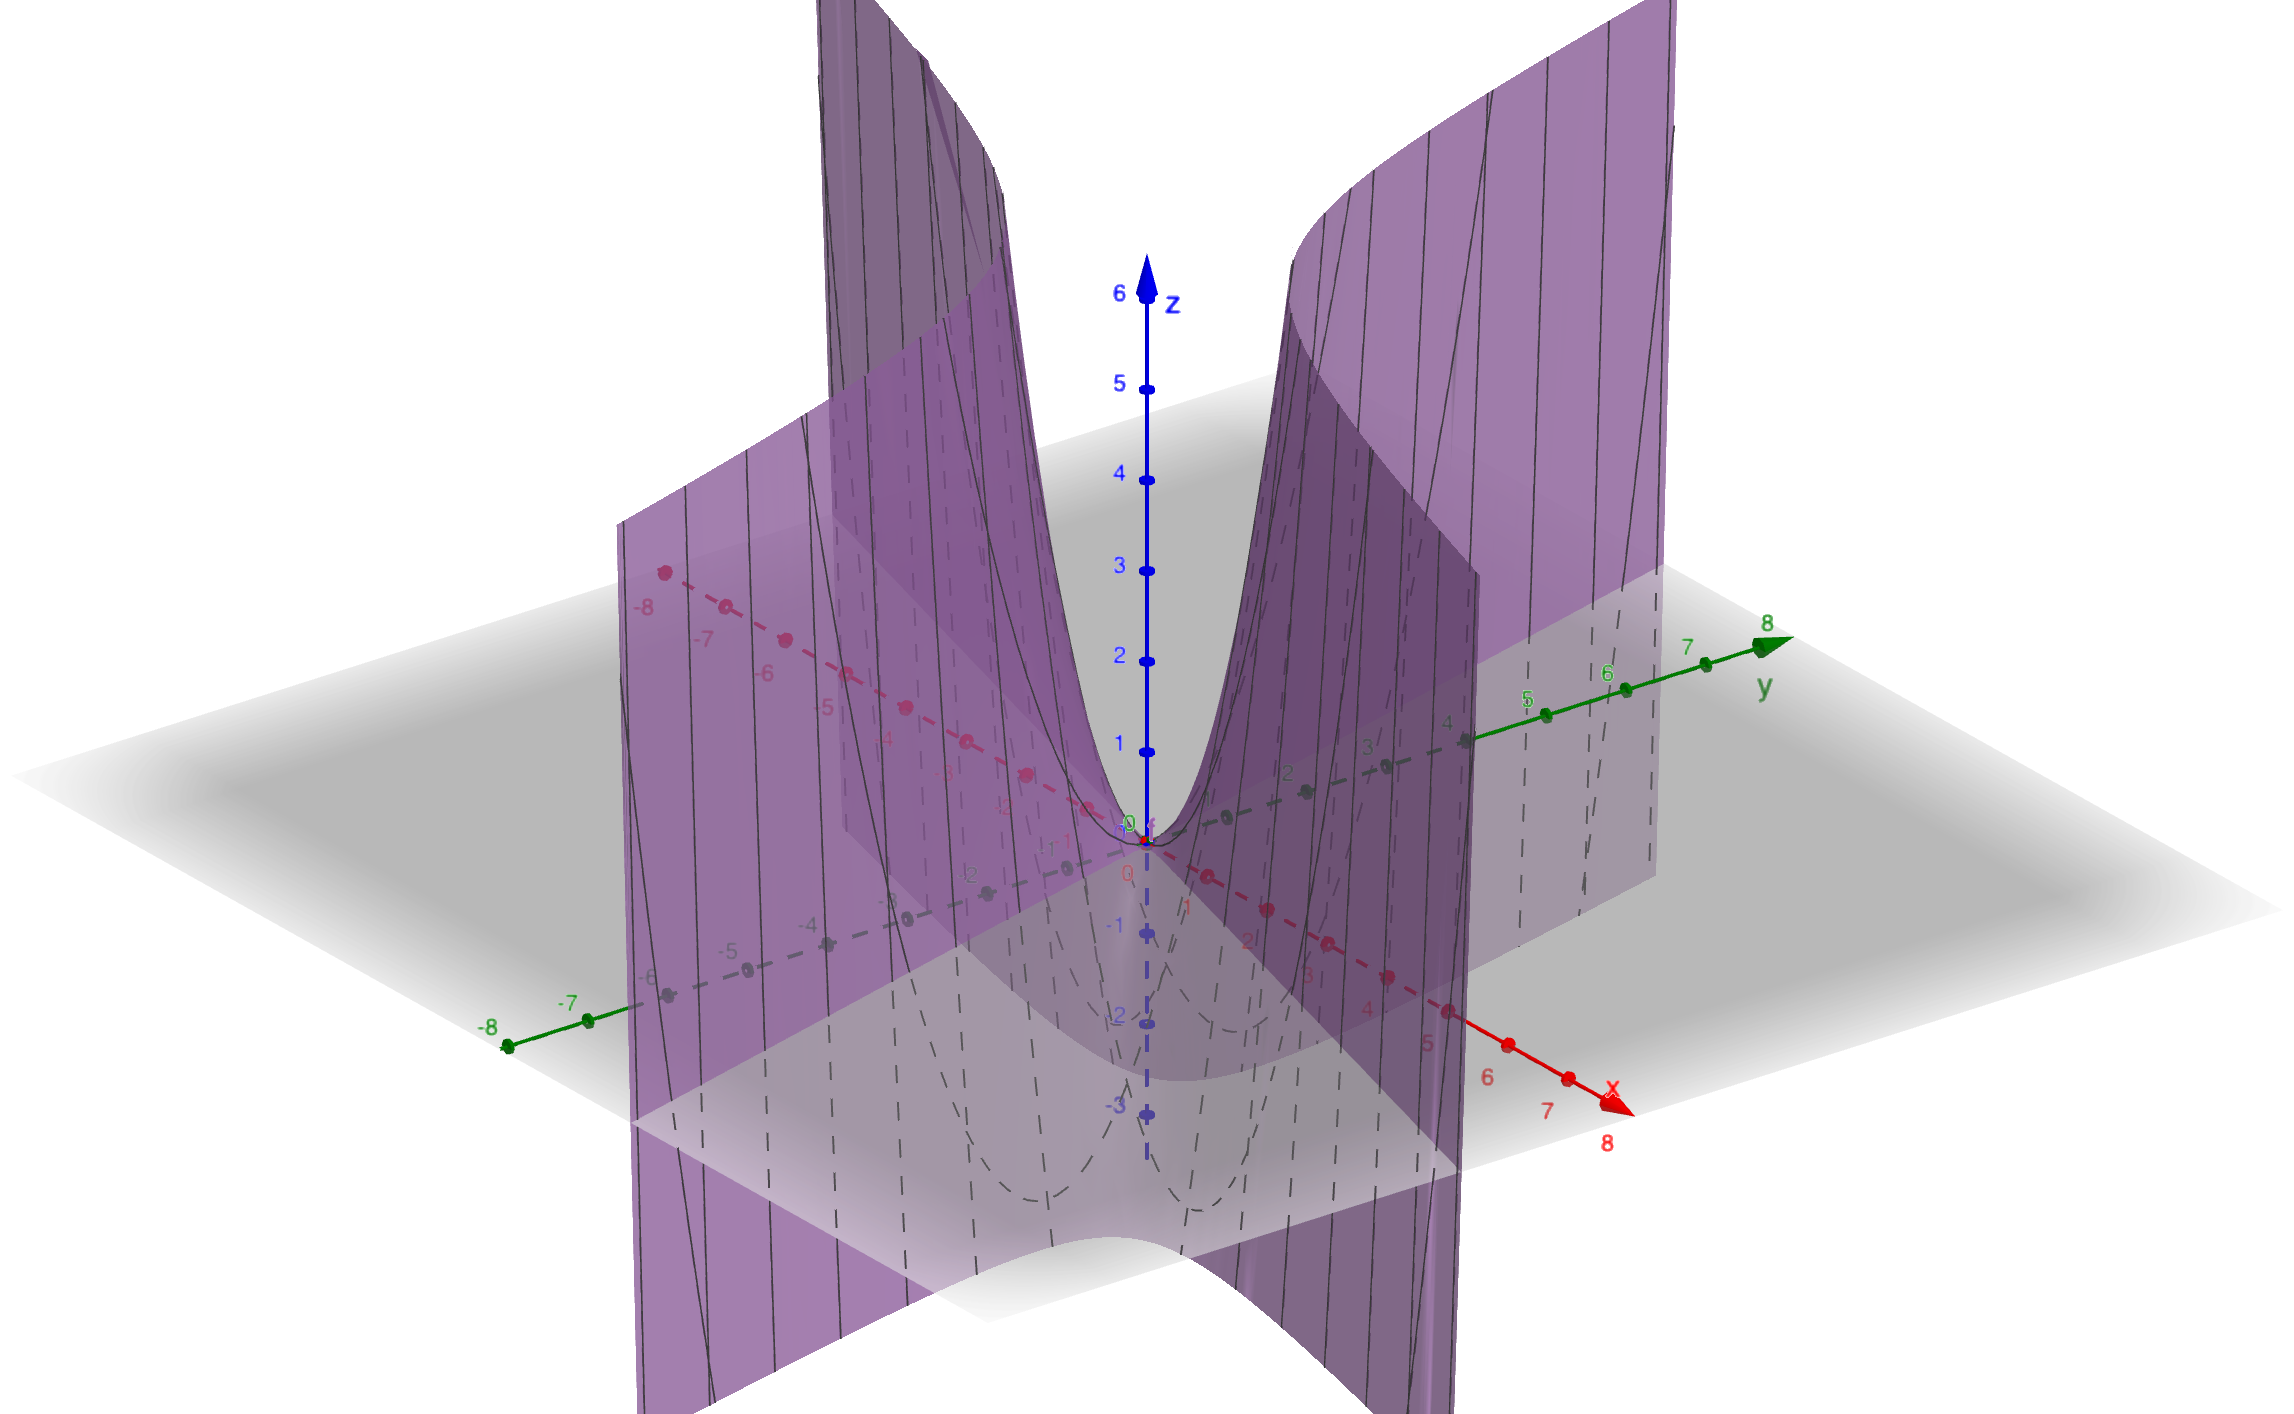
\includegraphics[width = 0.8 \textwidth]{media/introKriterien.png}
\end{center}



Betrachtet man den Graphen, so erkennt man das Problem: Die Schnittkurven in \(x\)- und \(y\)-Richtung weisen in der Tat ein lokales Minimum auf. Schneidet man den Graphen jedoch entlang einer Winkelhalbierenden der beiden Achsen, so hat die entsprechende Schnittkurve an der Stelle \((0,0)\) ein lokales Maximum.

Das kann auch rechnerisch bestätigt werden: Für die Richtungsableitung in Richtung \(\vec{v}=\begin{pmatrix} 1 \\ -1 \end{pmatrix}\) gilt
\[
	\frac{\partial f}{\partial \vec{v}}(x, y) =\left\langle \vec\nabla f(x,y) , \begin{pmatrix} 1 \\ -1 \end{pmatrix} \right\rangle = -2x + 2y
\]
Somit gilt \(\frac{\partial f}{\partial \vec{v}}(0,0) = 0\). Das widerspiegelt die Tatsache, dass die Schnittkurve in diese Richtung an der Stelle \((0,0)\) eine horizontale Tangente aufweist. Wie steht es aber mit der zweiten Ableitung in diese Richtung? Dazu berechnen wir die Richtungsableitung in Richtung \(\vec{v}=\begin{pmatrix} 1 \\ -1 \end{pmatrix}\) der Funktion \(z = -2x + 2y\):
\[
	\frac{\partial \left( -2x + 2y \right)}{\partial \vec{v}}  = \left\langle \vec \nabla \left( -2x + 2y \right) , \begin{pmatrix} 1 \\ -1 \end{pmatrix} \right\rangle = \left\langle \begin{pmatrix} -2 \\ 2 \end{pmatrix}, \begin{pmatrix} 1 \\ -1 \end{pmatrix} \right\rangle = -4.
\]
In Richtung \(\vec{v}=\begin{pmatrix} 1 \\ -1 \end{pmatrix}\) ist die zweite Ableitung negativ! Damit weist die Schnittkurve in diese Richtung ein lokales Maximum auf!


\subsubsection*{Fazit}
Damit ein lokales Minimum vorliegt, muss die zweite Richtungsableitung in \textbf{jede} Richtung positiv sein! Die Richtungsableitungen zweiter Ordnung lassen sich einfach mit der Hesse-Matrix berechnen. Betrachten Sie dazu die folgende Lernaufgabe:

\begin{LA}
	{}{}
	\textbf{Ziel:} Nachvollziehen, dass die zweifache Ableitung der Funktion \(f\) in einer bestimmten Richtung \(\vec{v}\) das gleiche ist wie das Skalarprodukt \(\langle \vec{v} ,\, H \vec{v} \rangle\), wobei \(H\) die Hesse-Matrix von \(f\) ist.

	\textbf{Aufgabe:} Sei zunächst \(f(x,y) = x^3y - xy^2\).
	\begin{enumerate}
		\item Berechnen Sie \(\vec{\nabla} f(x,y)\) und \(H(x,y)\).
		\item Sei \(\vec{v} = \begin{pmatrix} v_1 \\ v_2 \end{pmatrix}\). %mit \(|\vec{v}| = 1\)
		      Berechnen Sie die Richtungsableitung \(\frac{\partial f}{\partial \vec{v}}(x, y)\) in Abhängigkeit der beiden Einträge \(v_1\) und \(v_2\).
		\item \(\frac{\partial f}{\partial \vec{v}}(x, y)\) ist wieder eine Funktion von \(\mathbb{R}^2\) nach \(\mathbb{R}\). Berechnen Sie deren Gradient \(\vec{\nabla}\left(\frac{\partial f}{\partial \vec{v}}(x, y)\right)\).
		\item Berechnen Sie \(H(x,y) \cdot \vec{v}\) und zeigen Sie, dass \(H(x,y) \cdot \vec{v} = \vec\nabla\left(\frac{\partial f}{\partial \vec{v}}(x, y)\right)\) ist.
		\item Begründen Sie schliesslich, dass die zweite Ableitung in Richtung $\vec{v}$ \(\frac{\partial^2 f}{\partial \vec{v}^2} = \frac{\partial }{\partial \vec{v}}\left(\frac{\partial f}{\partial \vec{v}}(x, y)\right)\) das gleiche wie das Skalarprodukt \(\langle \vec{v} ,\, H \vec{v} \rangle\) ist.
		\item Führen Sie die gesamte Rechnung nochmals mit einer allgemeinen Funktion \(f(x,y)\) durch.
	\end{enumerate}
\end{LA}


\clearpage

\begin{satz}
	{Richtungsableitung zweiter Ordnung}{}
	Sei \(f(x,y)\) eine zweimal differenzierbare Funktion. Sei \(H(x,y)\) die Hesse-Matrix der Funktion und sei \(\vec{v} \in \mathbb{R}^2\). Dann gilt für die zweite Ableitung von \(f\) in Richtung \(\vec{v}\):
	\[
		\frac{\partial^2 f}{\partial \vec{v}^2} = \langle \vec{v} ,\, H \vec{v} \rangle.
	\]
\end{satz}

\begin{proof}


	Sei \(\vec{v} = \begin{pmatrix} v_1 \\ v_2 \end{pmatrix}\). Dann gilt für die Richtungsableitung
	\[
		\frac{\partial f}{\partial \vec{v}}(x, y) = \left\langle \vec\nabla f(x,y) ,\, \vec{v} \right\rangle= \frac{\partial f}{\partial x}(x,y) \cdot v_1 + \frac{\partial f}{\partial y}(x,y) \cdot v_2.
	\]
	Der Gradient dieser Richtungsableitung ist
	\[
		\vec\nabla\left(\frac{\partial f}{\partial \vec{v}}(x, y)\right) =
		\begin{pmatrix}
			\frac{\partial^2 f}{\partial x^2}(x,y) \cdot v_1 + \frac{\partial^2 f}{\partial x \partial y}(x,y) \cdot v_2 \\
			\frac{\partial^2 f}{\partial y \partial x}(x,y) \cdot v_1 + \frac{\partial^2 f}{\partial y^2}(x,y) \cdot v_2
		\end{pmatrix}
		=
		\begin{pmatrix}
			\frac{\partial^2 f}{\partial x^2}(x,y)          & \frac{\partial^2 f}{\partial x \partial y}(x,y) \\
			\frac{\partial^2 f}{\partial y \partial x}(x,y) & \frac{\partial^2 f}{\partial y^2}(x,y)
		\end{pmatrix}
		\cdot
		\begin{pmatrix}
			v_1 \\ v_2
		\end{pmatrix}
		= H \vec{v}.
	\]
	Für die zweite Ableitung von \(f\) in Richtung \(\vec{v}\) gilt damit:
	\[
		\frac{\partial^2 f}{\partial \vec{v}^2}  = \left\langle \vec{v} , \vec\nabla\left(\frac{\partial f}{\partial \vec{v}}(x, y)\right) \right\rangle = \left\langle \vec{v} , H \vec{v} \right\rangle.
	\]

\end{proof}

Wenn also die Matrix \(H\) die Eigenschaft hat, dass \(\langle \vec{v} ,\, H \vec{v} \rangle > 0\) für alle \(\vec{v} \in \mathbb{R}^2\), dann sind alle Richtungsableitungen zweiter Ordnung positiv. Solche Matrizen haben einen speziellen Namen:

\begin{definition}
	{Positive Definitheit}{}
	Eine Matrix \(H\) heisst positiv definit, wenn für alle \(\vec{v} \in \mathbb{R}^2\) gilt:
	\[
		\langle \vec{v} ,\, H \vec{v} \rangle > 0.
	\]
	Eine Matrix \(H\) heisst negativ definit, wenn für alle \(\vec{v} \in \mathbb{R}^2\) gilt:
	\[
		\langle \vec{v} ,\, H \vec{v} \rangle < 0.
	\]
	Eine Matrix \(H\) heisst indefinit, wenn es \(\vec{v} \in \mathbb{R}^2\) gibt, so dass \(\langle \vec{v} ,\, H \vec{v} \rangle > 0\) und \(\vec{w} \in \mathbb{R}^2\) so dass \(\vec{w} \cdot H \vec{w} < 0\).

\end{definition}

Wenn die Funktion \(f(x,y)\) zweimal stetig differenzierbar ist, ist die Hesse-Matrix eine symmetrische \(2 \times 2\)-Matrix. Für solche lässt sich die Definitheit leicht erkennen. Es gilt:
\begin{satz}
	{Kriterium für Definitheit}{}
	Eine symmetrische Matrix \(H\) ist genau dann positiv definit, wenn \(\det(H) > 0\) und \(h_{11} > 0\). Analog ist eine symmetrische Matrix \(H\) genau dann negativ definit, wenn \(\det(H) > 0\) und \(h_{11} < 0\). Falls \(\det(H) < 0\), ist \(H\) indefinit.
\end{satz}

Beweis: siehe nächstes Kapitel\dots



Zusammengefasst erhalten wir die folgenden einigermassen handlichen Kriterien, um festzustellen, welche Art kritischer Punkt vorliegt:
\begin{satz}
	{Klassifikation der kritischen Punkte}{}
	Sei \(f(x,y)\) eine zweimal stetig differenzierbare Funktion. Sei \(K = (x_0,y_0)\) eine kritische Stelle von \(f\) und sei \(H(K)\) die Hesse-Matrix an dieser Stelle. Dann gilt:
	\begin{enumerate}
		\item Ist \(\det(H(K)) > 0\) und \(h_{11} > 0\), so liegt an der Stelle \(K\) ein lokales Minimum vor.
		\item Ist \(\det(H(K)) > 0\) und \(h_{11} < 0\), so liegt an der Stelle \(K\) ein lokales Maximum vor.
		\item Ist \(\det(H(K)) < 0\), so liegt an der Stelle \(K\) ein Sattelpunkt vor.
	\end{enumerate}
\end{satz}

\begin{ueb}
	{}{}

	\begin{enumerate}
		\item Betrachten Sie nochmals die Funktion \(f(x,y) = x^3 + xy^2 - x\). Der Gradient und die kritischen Stellen haben wir in \Cref{bsp:kritischePunkte2} bereits ermittelt:
		      \[
			      \nabla f(x,y) = \begin{pmatrix}
				      3x^2 + y^2 - 1 \\
				      2xy
			      \end{pmatrix}
		      \]
		      \[
			      K_1 = (0,1), \quad K_2 = (0,-1), \quad K_3 = \left(\frac{\sqrt{3}}{3}, 0\right), \quad K_4 = \left(-\frac{\sqrt{3}}{3}, 0\right)
		      \]
		      Bestimmen Sie die Art der kritischen Punkte.

		\item Bestimmen Sie die lokalen Extrema und Sattelpunkte der folgenden Funktionen:
		      \begin{enumerate}
			      \item \(f(x,y) = x^2 - y^2\)
			      \item \(h(x,y) = \frac{1}{y} - \frac{1}{x} - 4x + y\)
			      \item \(k(x,y) = 3 \ln(x) - xy^2 + 2(y-x)\)
			      \item \(l(x,y) = (x^2 - 2x)(y^2 - 2y)\)
			      \item \(m(x,y) = \frac{1}{2}x^2 - \frac{1}{3}y^3 - xy + x - y - 1\)
			      \item  \(g(x,y) = (x+y)^2\)
			      \item \(j(x,y) = (x-1)^3 + (y-1)^3 - 3(x-1)(y-1) + 1\) Hinweis: Ersetze \(x-1\) durch \(u\) und \(y-1\) durch \(v\).
		      \end{enumerate}

		\item Eine Seilerei produziert Hanfseile in Naturfarben und blaue Hanfseile. Die Anzahlen \(x_N\) und \(x_B\) verkaufter Seile jeder Art pro Stunde hängen dabei jeweils von den Preisen \(p_N\) und \(p_B\) beider Produktionsartikel ab:
		      \[
			      x_N = 8 - 2p_N + p_B, \quad x_B = 9 + 2p_N - 2p_B
		      \]
		      Die Kosten für die Produktion eines naturfarbenen Seils belaufen sich auf 2 CHF. Jene für ein blaues Seil liegen bei 3 CHF. Wie soll die Seilerei die Preise \(p_N\) und \(p_B\) ansetzen, damit die Gewinne möglichst hoch ausfallen?
	\end{enumerate}

\end{ueb}

\clearpage
\emph{Lösungen}
\begin{enumerate}
	\item

	      \begin{itemize}
		      \item An den Stellen \(K_1\) und \(K_2\) gibt es einen Sattelpunkt.
		      \item Bei \(K_3\) ein lokales Minimum.
		      \item Bei \(K_4\) ein lokales Maximum.
	      \end{itemize}

	\item
	      \begin{enumerate}
		      \item \[
			            S = (0,0,0)
		            \]

		      \item \[
			            S_1 = \left(\frac{1}{2}, 1, -2\right), \quad H = \left(\frac{1}{2}, -1, -6\right), \quad T = \left(-\frac{1}{2}, 1, 6\right), \quad S_2 = \left(-\frac{1}{2}, -1, 2\right)
		            \]
		      \item \[
			            S = (1, 1, 1), \quad T = (2, 2, 0)
		            \]

		      \item \[
			            S_1 = (0, 0, 0), \quad S_2 = (0, 2, 0), \quad S_3 = (2, 0, 0), \quad S_4 = (2, 2, 0), \quad H = (1, 1, 1)
		            \]

		      \item \[
			            S = \left(-1, 0, -\frac{3}{2}\right), \quad T = \left(-2, -1, -\frac{5}{3}\right)
		            \]
		      \item
		            \begin{itemize}
			            \item Da \(\det(H) = 0\) ist, lässt sich das auf herkömmliche Weise nicht bestimmen.
			            \item Offensichtlich sind aber alle Funktionswerte positiv ausser auf den Punkten mit \(y = -x\).
			            \item Es gibt also unendlich viele Tiefpunkte:
			                  \[
				                  T = (x, -x, 0)
			                  \]
		            \end{itemize}
		      \item \[
			            H = (1, 1, -1), \quad S = \left(\frac{1}{2}, 2, 1 - \ln(8)\right)
		            \]
	      \end{enumerate}

	\item
	      \begin{enumerate}
		      \item \[
			            G(p_N, p_B) = (p_N - 2)(8 - 2p_N + p_B) + (p_B - 3)(9 + 2p_N - 2p_B)
		            \]
		      \item Der Gewinn ist maximal für \(p_N = 9\) und \(p_B = 10\).
	      \end{enumerate}
\end{enumerate}


























\clearpage
\subsection{Beweis der Kriterien für Definitheit}
\label{sec:beweisKriterien}

In den Übungen haben Sie häufig die folgenden hinreichenden Bedingungen für die Definitheit von symmetrischen Matrizen verwendet:

\noindent\fbox{\parbox{\textwidth}{Eine symmetrische Matrix \(H\) ist genau dann positiv definit, wenn \(\det(H) > 0\) und \(h_{11} > 0\). \\
		Analog ist eine symmetrische Matrix \(H\) genau dann negativ definit, wenn \(\det(H) > 0\) und \(h_{11} < 0\). \\
		Falls \(\det(H) < 0\), ist \(H\) indefinit.}}

In diesem Abschnitt werden wir die erste der eingerahmten Aussagen beweisen. Die beiden anderen kann man ähnlich begründen.


Für den Beweis werden wir einige Vorkenntnisse aus der linearen Algebra und Vektorgeometrie aufgreifen:
\begin{itemize}
	\item Sei \(A\) eine \(2 \times 2\)-Matrix. Wenn ein Vektor \(\vec{v} \in \mathbb{R}^2\) und eine Zahl \(\lambda \in \mathbb{R}\) existieren, mit \(A\vec{v} = \lambda \vec{v}\), dann nennt man \(\vec{v}\) einen Eigenvektor der Matrix \(A\) zum Eigenwert \(\lambda\).
	\item Die Eigenwerte sind die Nullstellen des charakteristischen Polynoms \(\det(A - \lambda E)\).
	\item Eine \(2 \times 2\)-Matrix heisst diagonalisierbar, wenn sie zwei linear unabhängige Eigenvektoren hat.
	      % \item Das Skalarprodukt von zwei Vektoren, die den Winkel \(\varphi\) einschliessen, ist definiert als
	      % \[
	      % \langle \vec{a} , \, \vec{b} \rangle = |\vec{a}| \cdot |\vec{b}| \cdot \cos \varphi.
	      % \]
	\item Zwei Vektoren \(\vec{a}\) und \(\vec{b}\) stehen genau dann senkrecht aufeinander, wenn \(\langle \vec{a} , \, \vec{b} \rangle = 0\) ist.
	\item Sei \(\vec{a} = \begin{pmatrix} a_1 \\ a_2 \end{pmatrix}\) und \(\vec{b} = \begin{pmatrix} b_1 \\ b_2 \end{pmatrix}\) die Komponentendarstellung der Vektoren \(\vec{a}, \vec{b}\) bezüglich der Standardbasis. Dann gilt
	      \[
		      \langle \vec{a} , \, \vec{b} \rangle = a_1 b_1 + a_2 b_2.
	      \]
	\item Das Skalarprodukt ist bilinear. Das heisst, für alle \(\vec{v}_1, \vec{v}_2, \vec{v}_3, \vec{v}_4 \in \mathbb{R}^2\) und \(a, b, c, d \in \mathbb{R}\) gilt:
	      \[
		      \langle a\vec{v}_1 + b\vec{v}_2 , \,  c\vec{v}_3 + d\vec{v}_4 \rangle = ac \cdot\langle\vec{v}_1 , \vec{v}_3 \rangle + ad \cdot\langle \vec{v}_1 , \vec{v}_4\rangle + bc\cdot \langle \vec{v}_2 , \vec{v}_3\rangle + bd \cdot\langle \vec{v}_2 , \vec{v}_4\rangle.
	      \]
\end{itemize}




\clearpage
\begin{LA}
	{Beweis Teil 1}{beweisTeil1}

	Im Folgenden betrachten wir symmetrische $2 \times 2$ Matrizen der Form
	\[
		A = \begin{pmatrix}
			a & b \\
			b & c
		\end{pmatrix}, \quad a, b, c \in \mathbb{R},
	\]
	mit $\det(A) > 0$ und $a > 0$.

	\subsubsection*{Ziele}
	\begin{enumerate}
		\item Matrizen dieser Art sind immer diagonalisierbar.
		\item Beide Eigenwerte sind positiv.
	\end{enumerate}

	Für die folgenden Aufgaben nehmen wir zunächst an, dass $b \neq 0$ gilt.
	\begin{enumerate}
		\item Zeigen Sie, dass das charakteristische Polynom die Form \(p(\lambda) = \lambda^2 - (a+c)\lambda + ac - b^2\) hat.
		\item Bestimmen Sie die Diskriminante des charakteristischen Polynoms und zeigen Sie, dass diese ein Term der Form \(U^2 + V^2\) und damit immer positiv ist.
		      Daraus folgt, dass die Matrix immer zwei verschiedene Eigenwerte hat und somit diagonalisierbar ist.
	\end{enumerate}

	Daraus folgt, dass die Matrix immer zwei verschiedene Eigenwerte hat und somit diagonalisierbar ist. und somit haben wir das erste Ziel erreicht.

	Zum zweiten Ziel:

	Für die nächsten Fragen benötigen Sie den Satz von Vieta:

	Seien \(x_1\) und \(x_2\) die Lösungen der Gleichung \(x^2 + Bx + C = 0\). Dann gilt:
	\[
		x_1 \cdot x_2 = C \quad \text{und} \quad x_1 + x_2 = -B.
	\]

	\begin{enumerate}[resume]
		\item Seien \(\lambda_1\) und \(\lambda_2\) die beiden Eigenwerte der Matrix \(A\). Zeigen Sie mit dem Satz von Vieta, dass \(\lambda_1 \cdot \lambda_2 = \det(A)\) ist.

		      Weil wir Matrizen mit \(\det(A) > 0\) betrachten, folgt daraus, dass die beiden Eigenwerte das gleiche Vorzeichen haben!
		\item Sei weiter \(\det(A) > 0\) und \(a > 0\):
		      \begin{enumerate}
			      \item Zeigen Sie zunächst, dass dann auch \(c > 0\) sein muss.
			      \item Zeigen Sie anschliessend mit dem Satz von Vieta, dass beide Eigenwerte der Matrix positiv sind.
		      \end{enumerate}
		\item Zusatz: Begründen Sie, wieso die beiden unter «Ziele» aufgeführten Aussagen auch stimmen, wenn \(b = 0\) ist.
	\end{enumerate}


\end{LA}

\clearpage

\begin{LA}
	{Beweis Teil 2}{beweisTEil2}
	\noindent Im Folgenden betrachten wir symmetrische Matrizen, also solche der Form
	\[
		A = \begin{pmatrix}
			a & b \\
			b & c
		\end{pmatrix}, \quad a, b, c \in \mathbb{R},
	\]
	mit zwei reellen, unterschiedlichen Eigenwerten \(\lambda_1 \neq \lambda_2\).

	\subsubsection*{Ziel}
	Die Eigenvektoren solcher Matrizen stehen senkrecht aufeinander.

	\begin{enumerate}
		\item Seien \(\vec{u} = \begin{pmatrix} u_1 \\ u_2 \end{pmatrix}\) und \(\vec{w} = \begin{pmatrix} w_1 \\ w_2 \end{pmatrix}\) zwei beliebige Vektoren. Zeigen Sie, dass
		      \[
			      \langle A \vec{u}, \vec{w} \rangle = \langle \vec{u}, A \vec{w} \rangle,
		      \]
		      wobei \(\langle \cdot, \cdot \rangle\) das Skalarprodukt bezeichnet.\\
		      \textbf{Bemerkung:} Dies gilt nur für symmetrische Matrizen.

		\item Seien \(\vec{v}_1\) und \(\vec{v}_2\) die Eigenvektoren der Matrix zu den Eigenwerten \(\lambda_1 \neq \lambda_2\). Begründen Sie jedes Gleichheitszeichen in der folgenden Rechnung:
		      \[
			      \lambda_1 \langle \vec{v}_1, \vec{v}_2 \rangle = \langle \lambda_1 \vec{v}_1, \vec{v}_2 \rangle = \langle A \vec{v}_1, \vec{v}_2 \rangle = \langle \vec{v}_1, A \vec{v}_2 \rangle = \langle \vec{v}_1, \lambda_2 \vec{v}_2 \rangle = \lambda_2 \langle \vec{v}_1, \vec{v}_2 \rangle.
		      \]

		\item Vergleichen Sie den Term ganz links mit jenem ganz rechts in der Gleichung oben und begründen Sie damit, dass die Eigenvektoren senkrecht aufeinander stehen.
	\end{enumerate}
\end{LA}


\clearpage

\begin{LA}
	{Beweis Teil 3}{beweisTeil3}
	\noindent Im Folgenden betrachten wir symmetrische $2 \times 2$ Matrizen, die diagonalisierbar sind, lauter positive Eigenwerte haben und deren Eigenvektoren senkrecht aufeinander stehen.

	\subsubsection*{Ziel}
	Wir wollen zeigen, dass eine solche Matrix positiv definit ist.

	\begin{enumerate}
		\item Sei \(A = \frac{1}{5} \begin{pmatrix} 14 & 2 \\ 2 & 11 \end{pmatrix}\). Zeigen Sie, dass \(\vec{v}_1 = \begin{pmatrix} 1 \\ -2 \end{pmatrix}\) und \(\vec{v}_2 = \begin{pmatrix} 2 \\ 1 \end{pmatrix}\) Eigenvektoren der Matrix sind, und weisen Sie nach, dass diese Matrix alle in der Voraussetzung genannten Eigenschaften besitzt.

		\item Sei nun \(\vec{w}\) ein beliebiger Vektor in \(\mathbb{R}^2\). Da die beiden Eigenvektoren der Matrix \(A\) linear unabhängig sind, lässt sich jeder Vektor in \(\mathbb{R}^2\) als Linearkombination der beiden Eigenvektoren angeben. Es gibt also zwei Zahlen \(\alpha, \beta \in \mathbb{R}\), sodass
		      \[
			      \vec{w} = \alpha \cdot \vec{v}_1 + \beta \cdot \vec{v}_2.
		      \]

		      \begin{enumerate}
			      \item Zeigen Sie, dass \(A \vec{w} = 2\alpha \cdot \vec{v}_1 + 3\beta \cdot \vec{v}_2\) ist.

			      \item Verwenden Sie die Bilinearität des Skalarprodukts und zeigen Sie, dass
			            \[
				            \langle \vec{w}, A \vec{w} \rangle = 10\alpha^2 + 15\beta^2.
			            \]

			      \item Wie genau fliessen die Eigenwerte und die Komponenten der Eigenvektoren in die Rechnung oben ein? Oder anders gefragt: Wie setzen sich die Zahlen \(10\) und \(15\) zusammen?

			      \item Begründen Sie, wieso auch jede andere Matrix mit den in der Voraussetzung genannten Eigenschaften immer positiv definit ist.
		      \end{enumerate}
	\end{enumerate}
\end{LA}

\clearpage
\subsubsection*{Zusammenfassung der Ergebnisse}

Die folgenden Überlegungen gelten für eine Stelle \((x_0, y_0)\) mit \(\vec{\nabla} f(x_0, y_0) = \vec{0}\), \(\det(H(x_0, y_0)) > 0\) und \(\frac{\partial^2 f}{\partial x^2}(x_0, y_0) > 0\):
\begin{itemize}
	\item Aus \(\vec{\nabla} f(x_0, y_0) = \vec{0}\) folgt, dass die Richtungsableitung in jede Richtung \(\vec{v}\) Null ist, weil
	      \[
		      \frac{\partial f}{\partial\vec{v}} (x_0,y_0) = \langle \vec{\nabla} f(x_0, y_0), \vec{v} \rangle = \langle \vec{0}, \vec{v} \rangle = 0.
	      \]

	\item Für die zweifache Richtungsableitung von \(f\) in Richtung \(\vec{v}\) gilt:
	      \[
		      \frac{\partial^2 f}{\partial\vec{v}^2}  = \langle \vec{v}, H \vec{v} \rangle.
	      \]

	\item Aus \(\det(H(x_0, y_0)) > 0\) und \(\frac{\partial^2 f}{\partial x^2}(x_0, y_0) > 0\) folgt (Teile 1-3), dass die Matrix \(H(x_0, y_0)\) positiv definit ist, also dass für jeden Vektor \(\vec{v}\) gilt:
	      \[
		      \langle \vec{v}, H \vec{v} \rangle > 0.
	      \]

	\item Der Graph von \(f\) hat demnach in jede Richtung \(\vec{v} = \begin{pmatrix} v_1 \\ v_2 \end{pmatrix}\) ein lokales Minimum. Damit meint man:
	      \begin{itemize}
		      \item Die Funktion \(t \mapsto f((x_0, y_0) + t \cdot (v_1, v_2))\) hat für jede Wahl von \((v_1, v_2) \in \mathbb{R}^2\) an der Stelle \(t = 0\) ein lokales Minimum.
		      \item Schneidet man den Graphen von \(f\) mit einer beliebigen Ebene, die durch den Punkt \((x_0, y_0, 0)\), parallel zur \(z\)-Achse und parallel zu \(\vec{v}\) verläuft, so entsteht eine Schnittkurve, die unabhängig von der Wahl von \(\vec{v} \in \mathbb{R}^2\) an der Stelle \((x_0, y_0)\) ein lokales Minimum hat.
	      \end{itemize}

	\item Das Bild unten zeigt den Graphen einer Funktion und den Schnitt mit einer Ebene durch den Tiefpunkt parallel zur \(z\)-Achse:
\end{itemize}
\begin{center}
	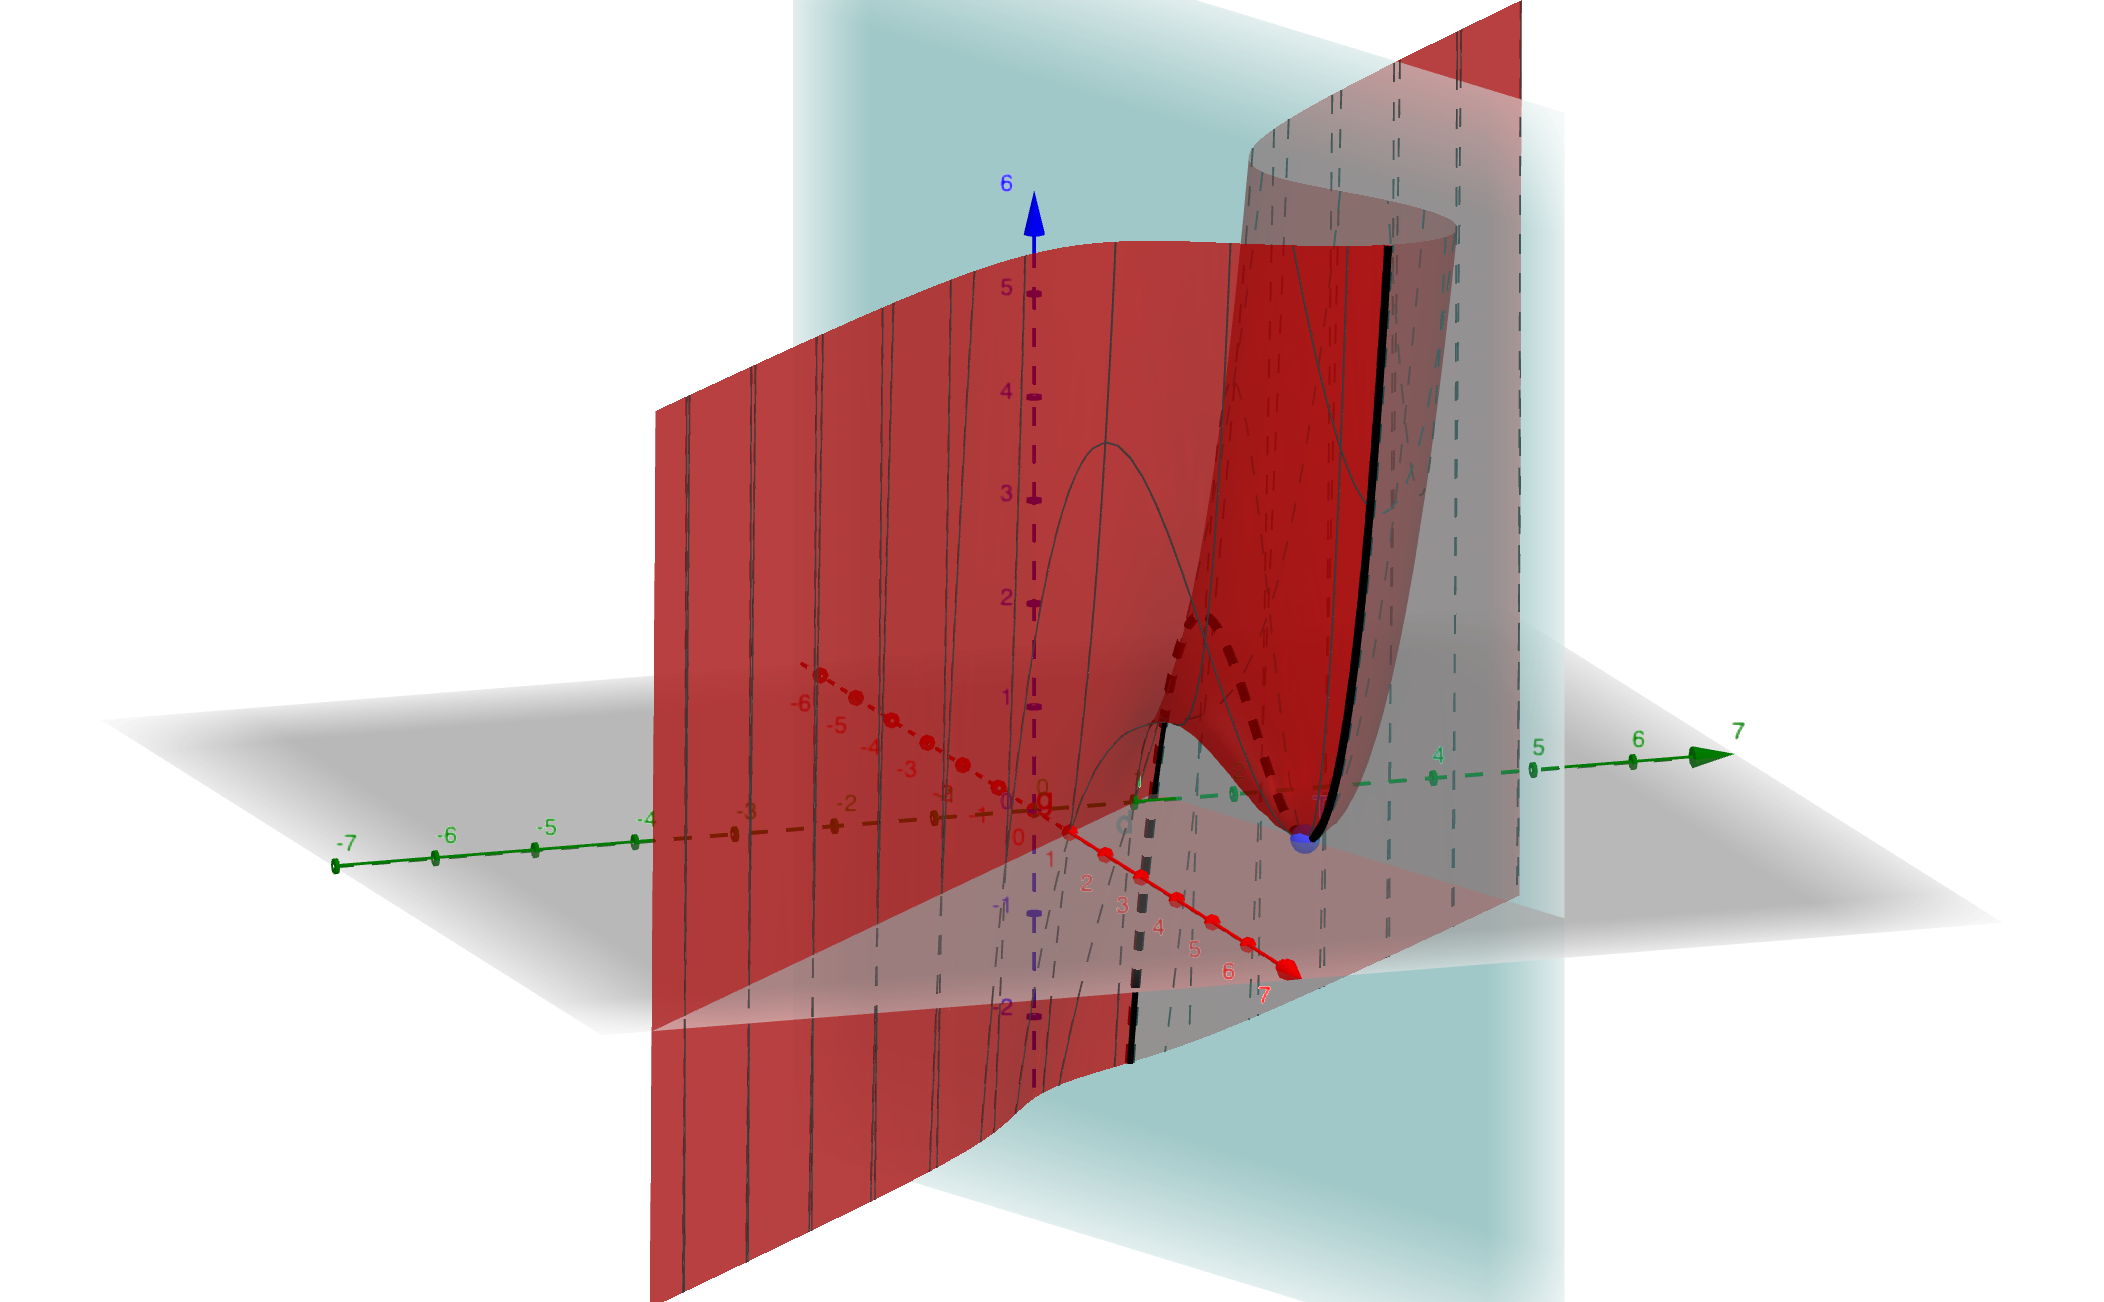
\includegraphics[width = 0.8\textwidth]{media/KriterienSchnitteneu.png}
\end{center}

\clearpage
\section{Die Methode der kleinsten Quadrate}

In Anwendungssituationen wird man kaum erreichen, dass Modell und Messdaten exakt zusammenpassen. Ein Modell, das die Daten exakt interpoliert, wird in den seltensten Fällen ein brauchbares Modell sein.

Betrachten Sie dazu das folgende Beispiel. Ein Autofahrer hat mehrmals die mit seinem Auto getankte Benzinmenge und die gefahrenen Kilometer notiert:

\begin{center}
\begin{tabular}{|c|c|c|c|c|c|c|c|c|c|}
\hline
% \textbf{} & \textbf{1} & \textbf{2} & \textbf{3} & \textbf{4} & \textbf{5} & \textbf{6} & \textbf{7} & \textbf{8} & \textbf{9} \\
% \hline
\textbf{Strecke [km]} & 202 & 480 & 361 & 220 & 249 & 348 & 512 & 187 & 471 \\
\hline
\textbf{Benzin [l]} & 22.9 & 45.9 & 31.5 & 23.9 & 26.0 & 33.9 & 44.9 & 17.9 & 43.5 \\
\hline
\end{tabular}
\end{center}

\begin{center}
    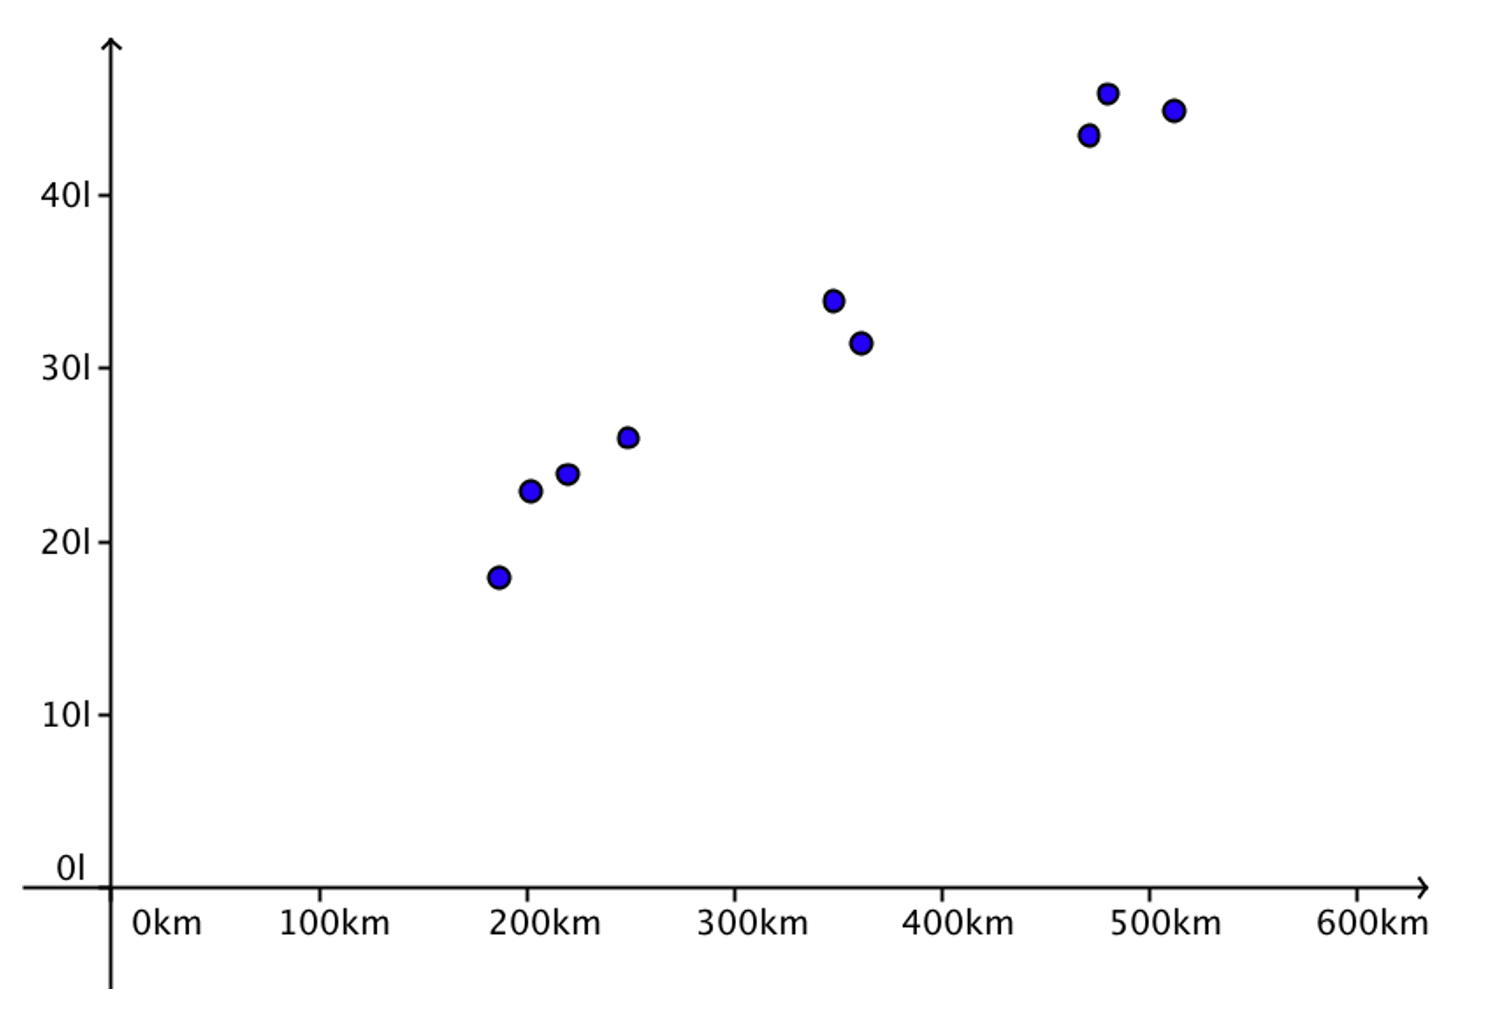
\includegraphics[width=0.5\textwidth]{media/introkleinsteQuadrate1.png}
\end{center}

Die 9 Messpunkte können durch eine Polynomfunktion 8. Grades exakt interpoliert werden. Die entsprechende Kurve sieht dann wie folgt aus:

\begin{center}
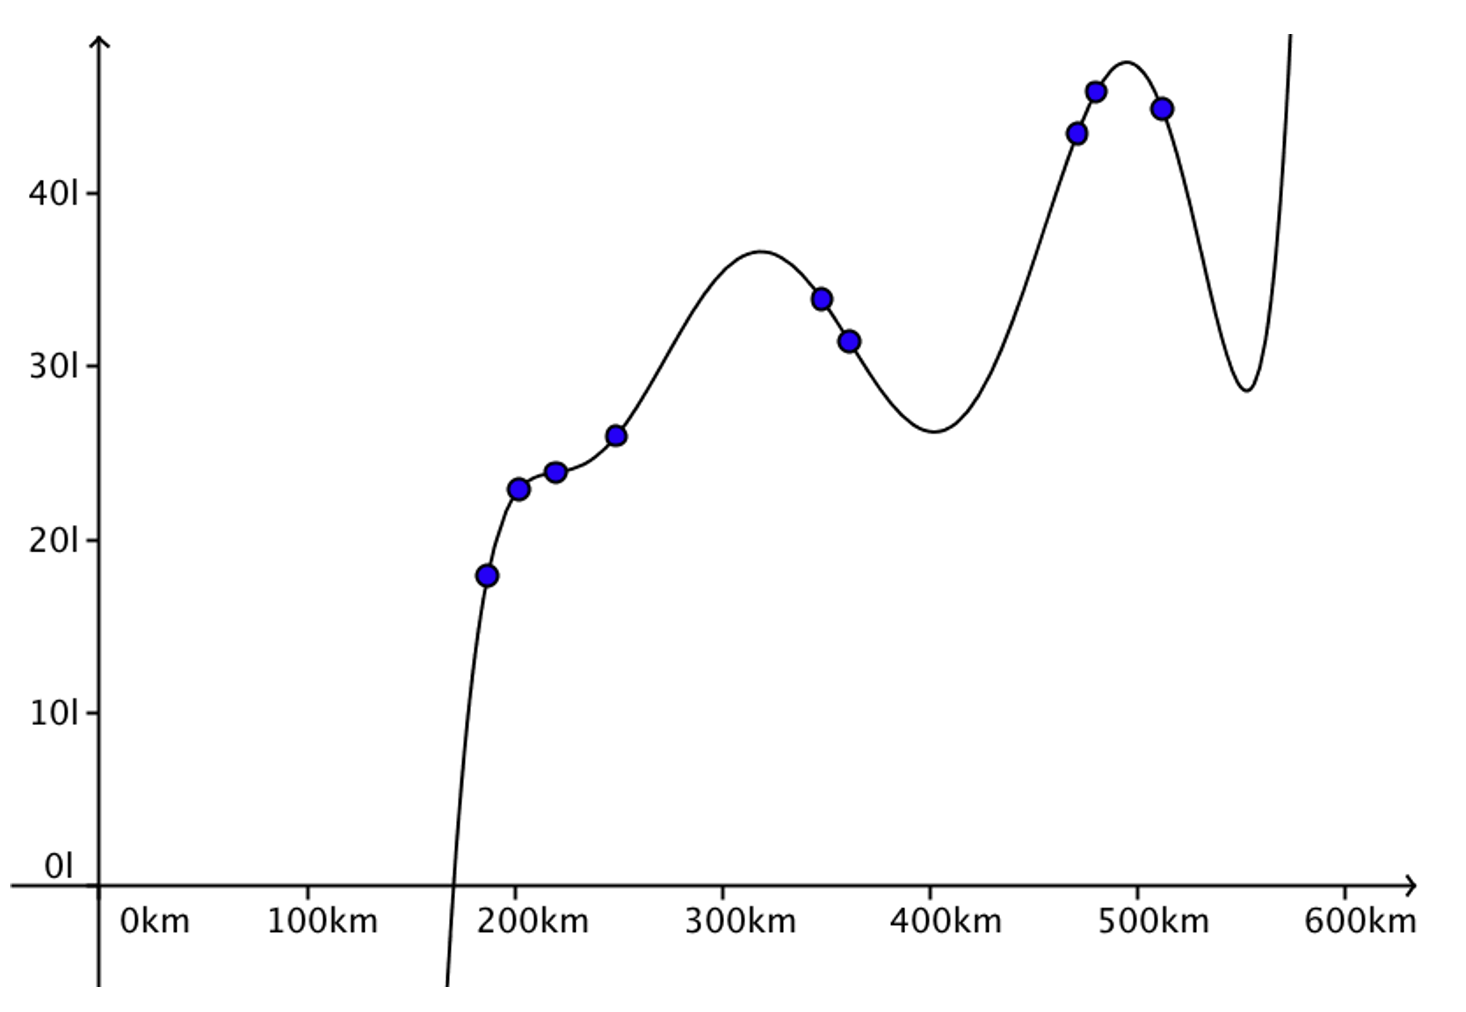
\includegraphics[width=0.5\textwidth]{media/introkleinstequadrate2.png}
\end{center}

Auch wenn das Polynom eine exakte Anpassung an die Messwerte leistet, so liefert es ein absurdes Modell. In diesem Fall ist es sinnvoll, von einem linearen Zusammenhang oder gar einer Proportionalität auszugehen. Damit lassen sich weitaus bessere Vorhersagen treffen. Das folgende Bild zeigt eine lineare Funktion, die sich den Messdaten annähert:

\begin{center}
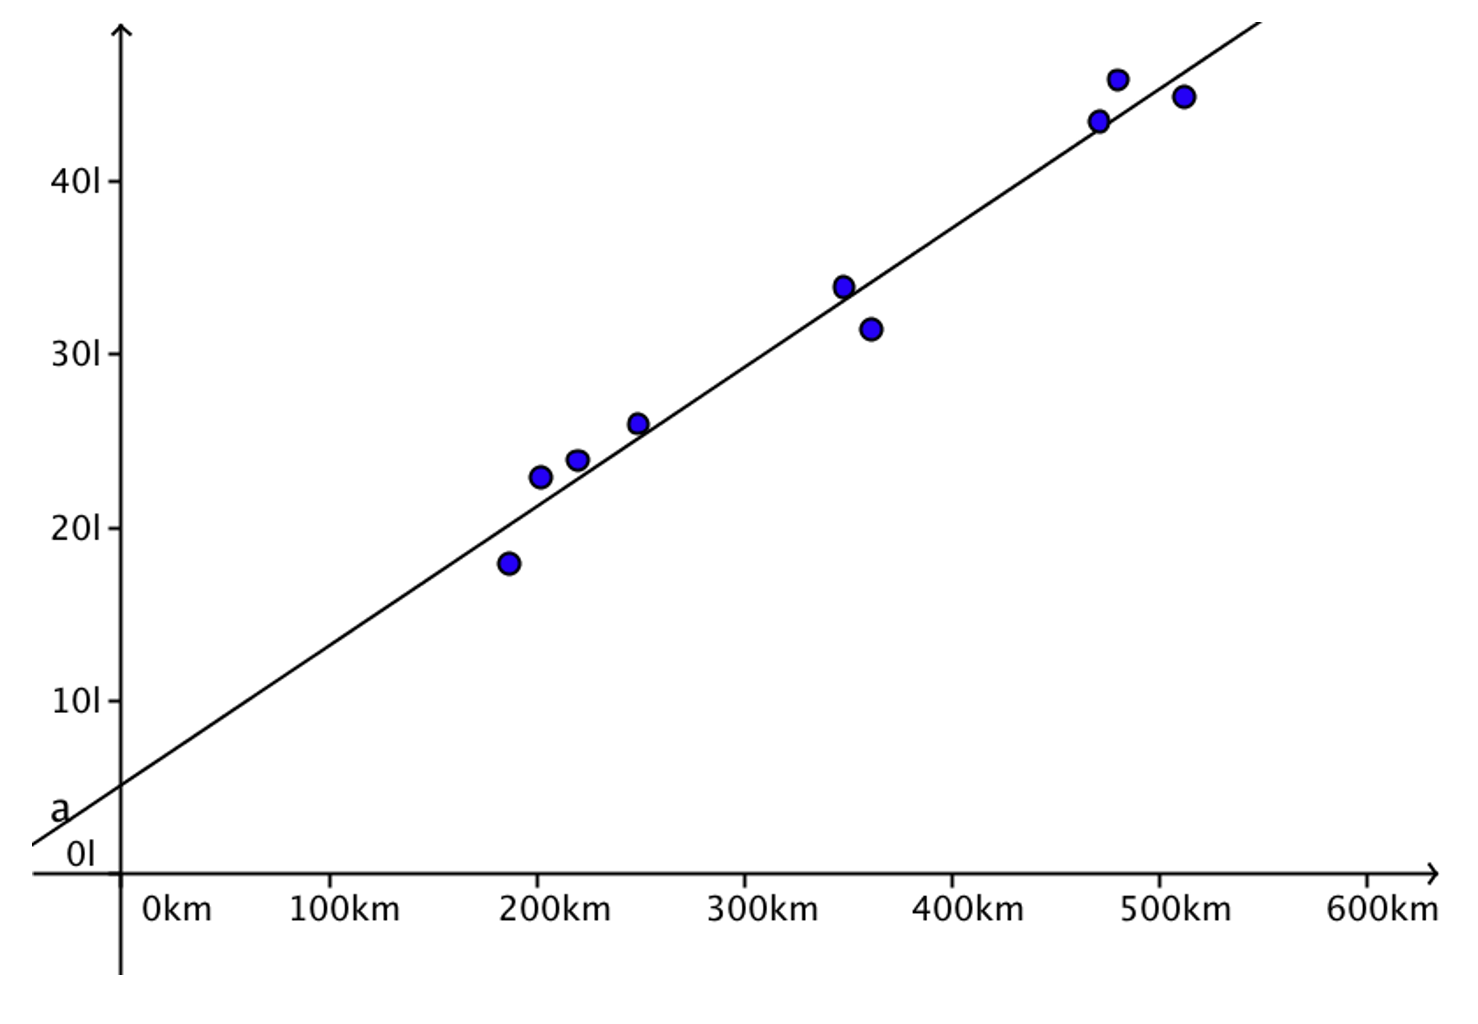
\includegraphics[width=0.5\textwidth]{media/introkleinstequadrate3.png}
\end{center}

Die Gerade in der Abbildung nennt man Regressionsgerade oder Ausgleichsgerade. Vielleicht haben Sie die Formel dafür bereits einmal angetroffen:

\begin{satz}
{Regressionsgerade}{}
Seien \( n \) Punkte \( P_1 (x_1, y_1), P_2 (x_2, y_2), \dots, P_n (x_n, y_n) \) gegeben.  
Die Gerade, welche sich im Sinne der kleinsten Quadrate den Punkten am besten nähert, ist \( g: y = mx + q \), mit  
\[
m = \frac{\sum_{k=1}^n (y_k - \overline{y}) x_k}{\sum_{k=1}^n (x_k - \overline{x}) x_k}, \quad q = \overline{y} - m \overline{x},
\]
wobei  
\[
\overline{x} = \frac{1}{n} \sum_{k=1}^n x_k, \quad \overline{y} = \frac{1}{n} \sum_{k=1}^n y_k
\]
die Mittelwerte der \( x \)- und \( y \)-Koordinaten der gegebenen Punkte sind.  
Die Gerade \( g \) nennt man \textbf{Regressions- oder Ausgleichsgerade}.
\end{satz}


In diesem Kapitel werden wir die Formel für die Regressionsgerade herleiten. Dabei werden wir unser Wissen über Extrema von Funktionen in zwei Variablen anwenden. Ausserdem werden wir ein allgemeines Prinzip kennenlernen, das viel weitreichender ist, als die Formel für die Ausgleichsgerade – die \textbf{Methode der kleinsten Quadrate}.

Diese Formel für die Regressionsgerade müssen Sie nicht lernen, die Methode der kleinsten Quadrate aber schon!

Um dieses Prinzip zu verstehen, werden wir so tun, als würden wir die Formel für die Regressionsgerade nicht kennen und in einem Beispiel mit wenigen Messpunkten eine passende lineare Funktion suchen.















\clearpage
\begin{LA}
{Methode der kleinsten Quadrate}{kleinsteQuadrate}
\textbf{Gegeben}: Messpunkte \( A(0,0), B(1,1), C(2,1), D(3,2) \)  

\textbf{Gesucht}: Eine lineare Funktion \( f(x) = mx + q \), die sich den Punkten annähert.

\begin{center}
    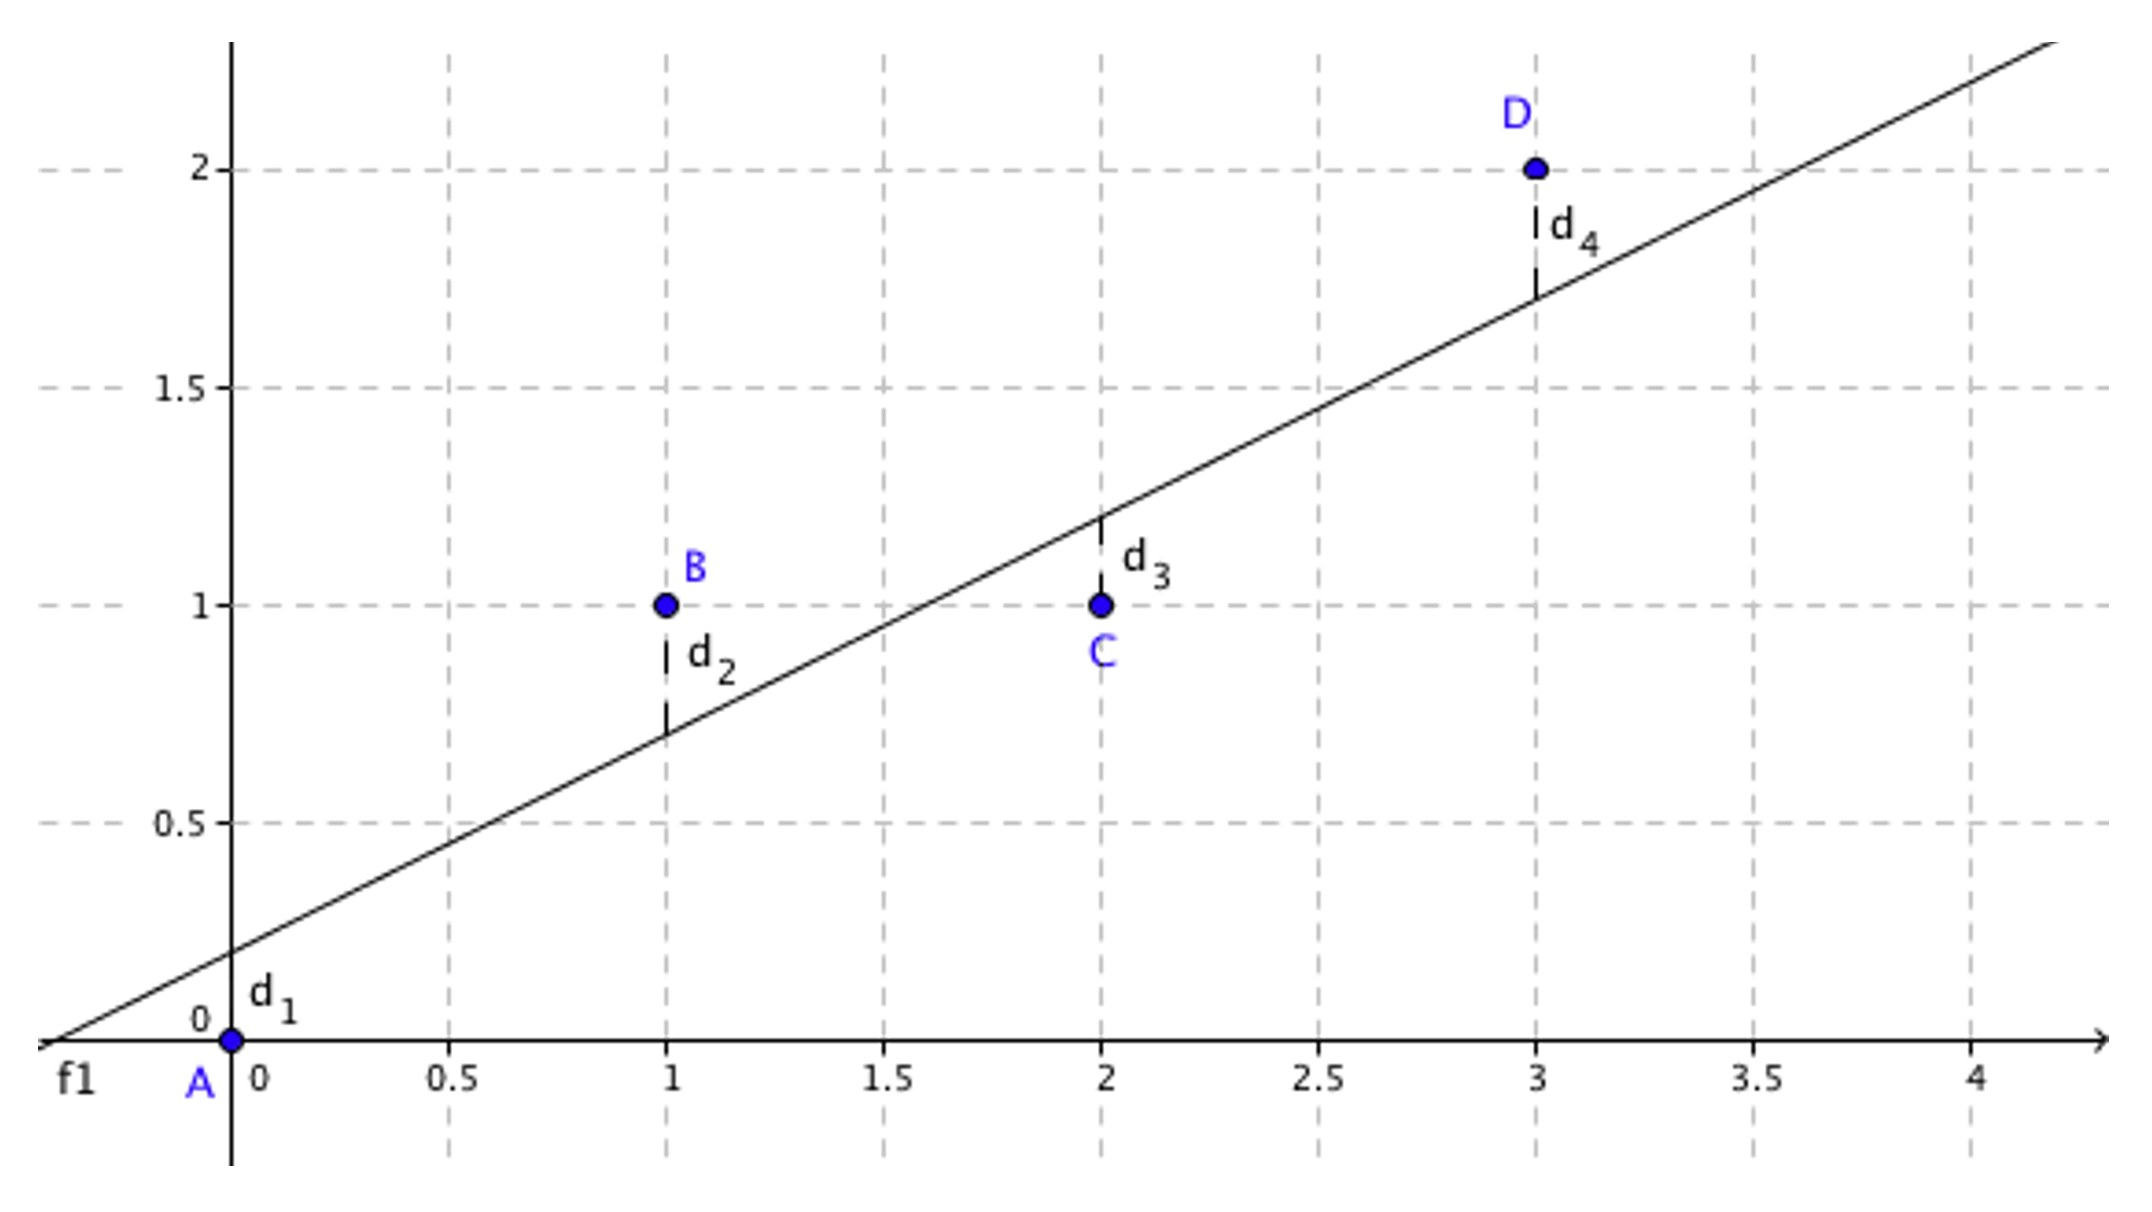
\includegraphics[width = 0.5 \textwidth]{media/kleinsteQuadrateLA.png}
\end{center}


\begin{enumerate}
    \item Betrachten Sie die Funktion \( f_1(x) = 0.5x + 0.2 \). Der Funktionswert an der Stelle \( x = 0 \) ist \( f_1(0) = 0.2 \). Der Messwert an der Stelle \( x = 0 \) ist 0 (siehe Punkt \( A \)). Die Abweichung beträgt also  
    \[
    d_1 = f_1(0) - 0 = 0.2 - 0 = 0.2
    \]
    Berechnen Sie analog die Abweichungen „Funktionswert minus Messwert“ \( d_2, d_3 \) und \( d_4 \) an den Stellen \( x = 1, x = 2 \) und \( x = 3 \). Wie gross ist die Summe der Abweichungen?  
    
    (Kontrolle: Summe \( = -0.2 \))
\end{enumerate}
\vspace*{4cm}



Wenn Sie stur nach der Formel „Funktionswert minus Messwert“ gerechnet haben, sind die Abweichungen \( d_1 \) und \( d_3 \) positiv, während \( d_2 \) und \( d_4 \) negativ sind. Das hat zur Folge, dass sich die Fehler in der Summe der Abweichungen zum Teil aufheben. Um das zu vermeiden, berechnet man die Summe der \textbf{Quadrate} der Abweichungen.  

\begin{enumerate}[resume]
    \item Berechnen Sie die Summe der Quadrate der Abweichungen  
    \[
    E = d_1^2 + d_2^2 + d_3^2 + d_4^2
    \]
    für die Funktion \( f_1(x) = 0.5x + 0.2 \).  
    \vspace*{2cm}
    %(Kontrolle: \( E = 0.26 \))


    \item Berechnen Sie die Summe der Quadrate der Abweichungen für die Funktionen \( f_2(x) = \frac{2}{3}x \) und \( f_3(x) = 1 \). Welche der Funktionen \( f_1, f_2 \) oder \( f_3 \) nähert sich den Punkten demnach am besten?  

    %(Kontrolle: \( E_2 = 0.\overline{2}, E_3 = 2 \))
\end{enumerate}


\vspace*{3cm}
Gibt es lineare Funktionen, welche für die vier vorgegebenen Punkte noch kleinere Summen von Abweichungsquadraten liefern als die vorgeschlagenen? Um diese Frage zu beantworten, betrachten wir eine allgemeine lineare Funktion \( f(x) = mx + q \).  

\begin{enumerate}[resume]
    \item Berechnen Sie für die vier vorgegebenen Punkte die Summe der Abweichungsquadrate \( E(m, q) \) in Abhängigkeit der Parameter \( m \) und \( q \).  
    
    (Kontrolle: \( E(m, q) = q^2 + (m + q - 1)^2 + (2m + q - 1)^2 + (3m + q - 2)^2 \))
    
\end{enumerate}
\vspace*{5cm}
%\clearpage
Wir wollen nun die Werte \( m \) und \( q \) bestimmen, für welche die Summe der Quadrate der Abweichungen \( E \) minimal wird.  


\begin{enumerate}[resume]
    \item An welcher Stelle \( (m, q) \) ist die Funktion \( E(m, q) \) minimal?  
    
    (Kontrolle: \( m = \frac{3}{5}, q = \frac{1}{10} \))
    %\vspace*{10cm}
\end{enumerate}
\end{LA}

\clearpage


\begin{definition}
{Methode der kleinsten Quadrate}{}
Seien \( n \) (Mess-)Punkte \( P_1 (x_1, y_1), P_2 (x_2, y_2), \dots, P_n (x_n, y_n) \) gegeben.

Sei $y=f(x)$ eine Funktion mit $k$ frei wählbare Parameter $a_1, a_2, \dots, a_k$.

Wir sagen, dass die Funktion $f(x)$ den Zusammenhang zwischen den Daten im Sinne der kleinsten Quadrate möglichst gut beschreibt, wenn die Parameter so gewählt sind, dass die Summe der quadrierten Abweichungen 

$$E(a_1, a_2 \dots, a_n) = \sum_{i=1}^n (f(x_i)- y_i)^2 $$

minimal ist.

\end{definition}

Bemerkungen:
\begin{itemize}
    \item Wenn man die Überlegung von \cref*{LA:kleinsteQuadrate} allgemein mit $n$ Messpunkten durchführt, erhält man die bekannte Formel für die Regressionsgerade.
    \item Vielleicht haben Sie es bemerkt: Wir haben die Methode der kleinsten Quadrate bereits einmal verwendet, um den Fehler im neuronalen Netzwerk zu minimieren.
\end{itemize}

\begin{ueb}
{}{}
\begin{enumerate}
    % \item Betrachten Sie die Messdaten:
    % \[
    % \begin{array}{|c|c|c|c|c|c|c|c|c|}
    % \hline
    % x & 1 & 3 & 4 & 6 & 8 & 9 & 11 & 14 \\
    % \hline
    % y & 1 & 2 & 4 & 4 & 5 & 7 & 8 & 9 \\
    % \hline
    % \end{array}
    % \]

    % \begin{enumerate}
    %     \item Bestimmen Sie die Regressionsgerade.

    %     \item Bestimmen Sie die Regressionsgerade, nachdem Sie die Rolle von \( x \) und \( y \) vertauscht haben.
    
    %     \item Zeichnen Sie die Punkte mit Excel in einem «xy-Diagramm». Unter den Diagrammoptionen können Sie eine Trendlinie hinzufügen und in den Einstellungen wählen, dass deren Gleichung angezeigt wird. Vergleichen Sie Ihr Resultat mit der Excel-„Trendlinie“.
    % \end{enumerate}
    
    
    \item Gegeben sind die vier Punkte \( A(-1 , 0), B(0 , 1), C(1 , 1), D(2 , -1) \).  
    Bestimmen Sie die Funktion
    $$f(x) = ax^2+bx+c ,$$
    die sich im Sinne der kleinsten Quadrate den Punkten am besten nähert.

    \item Gegeben \( n \) Punkte \( P_1 (x_1 , y_1), P_2 (x_2 , y_2), \dots, P_n (x_n , y_n) \).  \\ 
    Gesucht ist ein Kreis \( K: x^2 + y^2 = r^2 \) um den Ursprung mit Radius \( r \), der sich den Punkten nähert. Dabei soll der Radius \( r \) so gewählt werden, dass  
    \[
    E(r) = \sum_{k=1}^n \left( x_k^2 + y_k^2 - r^2 \right)^2
    \]
    minimal ist. Geben Sie eine Formel für \( r \) an. \footnote{Auf eine ähnliche Art konnte Gauss im Jahr 1801 die Bahn des Zwergplaneten Ceres berechnen. Weil seine Voraussagen viel präziser als jene der führenden Astronomen war, hat der 24 jährige Gauss damit einiges Aufsehen erregt!}
\end{enumerate}
    
\end{ueb}

\clearpage
\emph{Lösungen}
\begin{enumerate}
    % \item \textbf{Regressionsgerade:}
    % \begin{enumerate}
    %     \item \( y = \frac{7}{11}x + \frac{6}{11} \)
    %     \item \( y = \frac{3}{2}x - \frac{1}{2} \) (Weil die Abweichungen in senkrechter Richtung gemessen werden, spielt es eine Rolle, welche Werte als In- und welche als Output interpretiert werden.)
    %     \item Die Trendlinie entspricht genau der Regressionsgerade.
    % \end{enumerate}

    \item \textbf{Ansatz:} \( y = ax^2 + bx + c \). Die Gleichung \( \vec \nabla E(a, b, c) = 0 \) ist ein \( 3 \times 3 \)-System mit genau einer Lösung. Diese muss ein Minimum sein. Die gesuchte Parabel hat die Gleichung:
    \[
    y = -\frac{3}{4}x^2 + \frac{9}{20}x + \frac{23}{20}
    \]

    \item \( R = \pm \sqrt{\frac{\sum (x_k^2 + y_k^2)}{n}} \), wobei die negative Lösung als Radius wegfällt.
\end{enumerate}



\end{document}